\chapter[Phonology]{Phonology\label{Para_2}}

Papuan Malay has 18 consonant phonemes and a basic five-\isi{vowel system}. The \isi{consonant system} consists of six stops, two affricates, two fricatives, four nasals, two liquids, and two approximants. The \isi{vowel system} includes two front and two back vowels, and one open central vowel. Papuan Malay shows a clear preference for disyllabic roots and for CV and CVC syllables; the maximal syllable is CCVC. Stress typically falls on the penultimate syllable, although lexical roots with ultimate stress are also attested in the corpus.



The description of Papuan Malay \isi{phonology} is based on a \isi{word list} of 1,117 lexical roots plus 380 items, \isi{historically derived} by (unproductive) \isi{affixation} of Malay roots. The 1,497 lexemes are extracted from the 2,458-item \isi{word list}, mentioned in §\ref{Para_1.11.6}. The native consonant and vowel phoneme inventories are presented in §\ref{Para_2.1}. The phonological changes that the consonant and vowel segments can undergo are discussed in §\ref{Para_2.2}. A number of surface phenomena are described in §\ref{Para_2.3}. The phonotactics of Papuan Malay are investigated in §\ref{Para_2.4}, including a discussion of the segment distribution and possible sequences, syllable structures, and stress patterns. As already mentioned in §\ref{Para_1.11.6}, the corpus also includes a large number of loanwords; so far 719 items of the 2,458-item \isi{word list} (29\%) have been identified. Papuan Malay has also adopted one loan segment, the voiceless labio-dental fricative /\textstyleChCharisSIL{f}/, and developed three substitution strategies to realize another \isi{non-native segment}, the voiceless postalveolar fricative /\textstyleChCharisSIL{ʃ}/. The non-native segments and loanwords are discussed in §\ref{Para_2.5}. Given the rather large percentage of loanwords, this discussion is rather detailed, including a description of the phonological and phonetic processes and the phonotactics attested in loanwords.



This chapter closes with an account of the orthographic conventions used in this grammar in §\ref{Para_2.6} and a summary in §\ref{Para_2.7}.\footnote{Two important sources for the description of the Papuan Malay \isi{phonology} are \citet{Donohue.2003} and \citet{SutriNarfafan.underreview}.}


\section{Segment inventory\label{Para_2.1}}
The Papuan Malay \isi{consonant system} is presented in §\ref{Para_2.1.1}, and the \isi{vowel system} in §\ref{Para_2.1.2}.


\subsection{Consonant system\label{Para_2.1.1}}
\subsubsection[Consonant inventory]{Consonant inventory\label{Para_2.1.1.1}}
Papuan Malay has 18 consonant phonemes, shown in \tabref{Table_2.1}. The system consists of three pairs of stops, one pair of affricates, four nasals, two fricatives, two liquids, and two approximants.

\begin{table}[h]
\caption{Papuan Malay \isi{consonant inventory}\label{Table_2.1}}
\begin{tabular}{lllllllllllll}
\lsptoprule 
 & \multicolumn{2}{l}{ \textsc{lab}} & \multicolumn{2}{l}{ \textsc{alv}} & \multicolumn{2}{l}{ \textsc{pal-alv}} & \multicolumn{2}{l}{ \textsc{pal}} & \multicolumn{2}{l}{ \textsc{vel}} & \multicolumn{2}{l}{ \textsc{glot}}\\

\midrule
\textsc{stop} & \textstyleChCharisSIL{p} & \textstyleChCharisSIL{b} & \textstyleChCharisSIL{t} & \textstyleChCharisSIL{d} &  &  &  &  & \textstyleChCharisSIL{k} & \textstyleChCharisSIL{g} &  & \\
\textsc{affr} &  &  &  &  & \textstyleChCharisSIL{t}\textstyleChCharisSIL{ʃ} & \textstyleChCharisSIL{d}\textstyleChCharisSIL{ʒ} &  &  &  &  &  & \\
\textsc{nas} &  & \textstyleChCharisSIL{m} &  & \textstyleChCharisSIL{n} &  &  &  & \textstyleChCharisSIL{ɲ} &  & \textstyleChCharisSIL{ŋ} &  & \\
\textsc{fric} &  &  & \textstyleChCharisSIL{s} &  &  &  &  &  &  &  & \textstyleChCharisSIL{h} & \\
\textsc{rhot} &  &  &  & \textstyleChCharisSIL{r} &  &  &  &  &  &  &  & \\
\textsc{lat-aprx} &  &  &  & \textstyleChCharisSIL{l} &  &  &  &  &  &  &  & \\
\textsc{aprx} &  &  &  &  &  &  &  & \textstyleChCharisSIL{j} &  & \textstyleChCharisSIL{w} &  & \\
\lspbottomrule 
\end{tabular}
\end{table}

The 18 phonemes and their realizations are presented in \tabref{Table_2.2}. The rhotic has three allophones; the phonological and phonetic processes involved in their \isi{variation} are discussed in §\ref{Para_2.2.2} and §\ref{Para_2.3.1.3}, respectively. The voiceless stops are typically unreleased in the coda position. However, when occurring in the word-final coda position before a pause, they can be slightly released.

\begin{table}
\caption{Papuan Malay stops\label{Table_2.2}}

\begin{tabular}{llll}
\lsptoprule
\multicolumn{2}{l}{ Phoneme} & \multicolumn{2}{l}{ Realization}\\
\midrule
Stop & /\textstyleChCharisSIL{p}/ & [\textstyleChCharisSIL{p}], & a voiceless bilabial stop\\
&  & [\textstyleChCharisSIL{p̚}], & an unreleased voiceless bilabial stop\\
& /\textstyleChCharisSIL{b}/ & [\textstyleChCharisSIL{b}], & a voiced bilabial stop\\
& /\textstyleChCharisSIL{t}/ & [\textstyleChCharisSIL{t}], & a voiceless alveolar stop\\
&  & [\textstyleChCharisSIL{t̚}], & an unreleased voiceless alveolar stop\\
& /\textstyleChCharisSIL{d}/ & [\textstyleChCharisSIL{d}], & a voiced alveolar stop\\
& /\textstyleChCharisSIL{k}/ & [\textstyleChCharisSIL{k}], & a voiceless velar stop\\
&  & [\textstyleChCharisSIL{k̚}], & an unreleased voiceless velar stop\\
& /\textstyleChCharisSIL{g}/ & [\textstyleChCharisSIL{g}], & a voiced velar stop\\
Affricate & /\textstyleChCharisSIL{ʧ}/ & [\textstyleChCharisSIL{ʧ}], & a voiceless palato-alveolar affricate\\
& /\textstyleChCharisSIL{d}\textstyleChCharisSIL{ʒ}/ & [\textstyleChCharisSIL{d}\textstyleChCharisSIL{ʒ}], & a voiced palato-alveolar affricate\\
Nasal & /\textstyleChCharisSIL{m}/ & [\textstyleChCharisSIL{m}], & a voiced bilabial nasal\\
& /\textstyleChCharisSIL{n}/ & [\textstyleChCharisSIL{n}], & a voiced alveolar nasal\\
& /\textstyleChCharisSIL{ɲ}/ & [\textstyleChCharisSIL{ɲ}], & a voiced palatal nasal\\
& /\textstyleChCharisSIL{ŋ}/ & [\textstyleChCharisSIL{ŋ}], & a voiced velar nasal\\
Fricative & /\textstyleChCharisSIL{s}/ & [\textstyleChCharisSIL{s}], & a voiceless alveolar fricative\\
& /\textstyleChCharisSIL{h}/ & [\textstyleChCharisSIL{h}], & a voiceless glottal fricative\\
Liquid & /\textstyleChCharisSIL{r}/ & [\textstyleChCharisSIL{r}], & a voiced alveolar trill\\
&  & [\textstyleChCharisSIL{r̥}], & a voiceless alveolar trill\\
&  & [\textstyleChCharisSIL{ɾ}], & a voiced alveolar tap\\
& /\textstyleChCharisSIL{l}/ & [\textstyleChCharisSIL{l}], & a voiced alveolar lateral\\
Approximant & /\textstyleChCharisSIL{j}/ & [\textstyleChCharisSIL{j}], & a voiced palatal approximant\\
& /\textstyleChCharisSIL{w}/ & [\textstyleChCharisSIL{w}], & a voiced labio-velar approximant\\
\lspbottomrule 
\end{tabular}
\end{table}

\subsubsection[Contrast between similar consonants]{Contrast between similar consonants\label{Para_2.1.1.2}}

Contrast between similar consonants is presented in minimal or near-minimal pairs in the following tables: in word-initial position in \tabref{Table_2.3}, in root-internal position in \tabref{Table_2.4a} and \tabref{Table_2.4b}, and in word-final position in \tabref{Table_2.5}. When (near-)minimal pairs could not be found, another word containing a contrasting consonant is given. Some segments have a restricted distribution; the palatal nasal, for instance, does not occur in the coda position (§\ref{Para_2.4.1}).

\begin{table}
\caption{Consonant contrast in word-initial position\label{Table_2.3}}

\begin{tabular}{lllll}
\lsptoprule 
\multicolumn{2}{l}{ Contrast} & Item & Orthogr. & Gloss\\

\midrule
\textstyleChCharisSIL{p{\Tilde}b{\Tilde}m} &  & [\textstyleChCharisSIL{ˈpu.lu}] & \textitbf{pulu} & ‘tens’\\
&  & [\textstyleChCharisSIL{ˈbu.lu}] & \textitbf{bulu} & ‘body hair’\\
&  & [\textstyleChCharisSIL{ˈmu.lʊt̚}] & \textitbf{mulut} & ‘mouth’\\
\textstyleChCharisSIL{t{\Tilde}d{\Tilde}n} & \textstyleChCharisSIL{t{\Tilde}d} & [\textstyleChCharisSIL{ˈtɔ̞ŋ}] & \textitbf{tong} & ‘1\textsc{pl}’\\
&  & [\textstyleChCharisSIL{ˈdɔ̞ŋ}] & \textitbf{dong} & ‘3\textsc{pl}’\\
& \textstyleChCharisSIL{t{\Tilde}n} & [\textstyleChCharisSIL{ˈti.kɐr}] & \textitbf{tikar} & ‘plaited mat’\\
&  & [\textstyleChCharisSIL{ˈni.ka}] & \textitbf{nika} & ‘marry officially’\\
& \textstyleChCharisSIL{d{\Tilde}n} & [\textstyleChCharisSIL{ˈdɛ.kɐt̚}] & \textitbf{dekat} & ‘near’\\
&  & [\textstyleChCharisSIL{ˈnɛ.kɐt̚}] & \textitbf{nekat} & ‘be determined’\\
\textstyleChCharisSIL{k{\Tilde}g} &  & [\textstyleChCharisSIL{ˈka.ja}] & \textitbf{kaya} & ‘like’\\
&  & [\textstyleChCharisSIL{ˈga.ja}] & \textitbf{gaya} & ‘manner’\\
\textstyleChCharisSIL{ʧ{\Tilde}dʒ{\Tilde}t}/\textstyleChCharisSIL{d} & \textstyleChCharisSIL{ʧ{\Tilde}dʒ} & [\textstyleChCharisSIL{ˈʧu.ɾɐŋ}] & \textitbf{curang} & ‘be dishonest’\\
&  & [\textstyleChCharisSIL{ˈdʒu.ɾɐŋ}] & \textitbf{jurang} & ‘steep decline’\\
& \textstyleChCharisSIL{ʧ{\Tilde}t} & [\textstyleChCharisSIL{ˈʧɐm.pʊr}] & \textitbf{campur} & ‘mix’\\
&  & [\textstyleChCharisSIL{ˈtɐm.pɐr}] & \textitbf{tampar} & ‘beat’\\
& \textstyleChCharisSIL{dʒ{\Tilde}d} & [\textstyleChCharisSIL{ˈdʒa.ɾi}] & \textitbf{jari} & ‘digit’\\
&  & [\textstyleChCharisSIL{ˈda.ɾi}] & \textitbf{dari} & ‘from’\\
\textstyleChCharisSIL{s{\Tilde}h} &  & [\textstyleChCharisSIL{ˈsɐn.tɐŋ}] & \textitbf{santang} & ‘coconut milk’\\
&  & [\textstyleChCharisSIL{ˈhɐn.tɐm}] & \textitbf{hantam} & ‘strike’\\
\textstyleChCharisSIL{m{\Tilde}n{\Tilde}ɲ} & \textstyleChCharisSIL{m{\Tilde}n} & [\textstyleChCharisSIL{ˈma.si}] & \textitbf{masi} & ‘still’\\
&  & [\textstyleChCharisSIL{ˈna.si}] & \textitbf{nasi} & ‘cooked rice’\\
& \textstyleChCharisSIL{m{\Tilde}ɲ} & [\textstyleChCharisSIL{ˈmɛ.mɐŋ}] & \textitbf{memang} & ‘indeed’\\
&  & [\textstyleChCharisSIL{ˈɲa.mɐŋ}] & \textitbf{nyamang} & ‘be comfortable’\\
& \textstyleChCharisSIL{n{\Tilde}ɲ} & [\textstyleChCharisSIL{ˈna.kɐl}] & \textitbf{nakal} & ‘be mischievous’\\
&  & [\textstyleChCharisSIL{ˈɲa.wa}] & \textitbf{nyawa} & ‘soul’\\
\textstyleChCharisSIL{l{\Tilde}r} &  & [\textstyleChCharisSIL{ˈra.wɐŋ}] & \textitbf{rawang} & ‘be haunted’\\
&  & [\textstyleChCharisSIL{ˈla.wɐŋ}] & \textitbf{lawang} & ‘oppose’\\
\textstyleChCharisSIL{j{\Tilde}ɲ} &  & [\textstyleChCharisSIL{ˈjɐŋ}] & \textitbf{yang} & ‘\textsc{rel}’\\
&  & [\textstyleChCharisSIL{ˈɲa.wa}] & \textitbf{nyawa} & ‘soul’\\
\textstyleChCharisSIL{j{\Tilde}w} &  & [\textstyleChCharisSIL{ˈjɐŋ}] & \textitbf{yang} & ‘\textsc{rel}’\\
&  & [\textstyleChCharisSIL{ˈwa.ɾʊŋ}] & \textitbf{warung} & ‘food stall’\\
\lspbottomrule
\end{tabular}
\end{table}

\begin{table}

\caption{Consonant contrast in root-internal position\label{Table_2.4a}}

\begin{tabular}{lllll}
\lsptoprule
\multicolumn{2}{l}{Contrast} & Item & Orthogr. & Gloss\\

\midrule
\textstyleChCharisSIL{p{\Tilde}b{\Tilde}m} & \textstyleChCharisSIL{p{\Tilde}b} & [\textstyleChCharisSIL{ˈkɛ.pʊŋ}] & \textitbf{kepung} & ‘surround’\\
&  & [\textstyleChCharisSIL{ˈkɛ.bʊŋ}] & \textitbf{kebung} & ‘garden’\\
& \textstyleChCharisSIL{p{\Tilde}m} & [\textstyleChCharisSIL{ˈra.pi}] & \textitbf{rapi} & ‘be neat’\\
&  & [\textstyleChCharisSIL{ˈra.mɛ}] & \textitbf{rame} & ‘be bustling’\\
& \textstyleChCharisSIL{b{\Tilde}m} & [\textstyleChCharisSIL{ˈsu.bʊr}] & \textitbf{subur} & ‘be fertile’\\
&  & [\textstyleChCharisSIL{ˈsu.mʊr}] & \textitbf{sumur} & ‘(a) well’\\
\textstyleChCharisSIL{t{\Tilde}d{\Tilde}n} & \textstyleChCharisSIL{t{\Tilde}d} & [\textstyleChCharisSIL{ˈhi.tʊŋ}] & \textitbf{hitung} & ‘count’\\
&  & [\textstyleChCharisSIL{ˈhi.dʊŋ}] & \textitbf{hidung} & ‘nose’\\
& \textstyleChCharisSIL{t{\Tilde}n} & [\textstyleChCharisSIL{ˈbu.tu}] & \textitbf{butu} & ‘need’\\
&  & [\textstyleChCharisSIL{ˈbu.nu}] & \textitbf{bunu} & ‘kill’\\
& \textstyleChCharisSIL{d{\Tilde}n} & [\textstyleChCharisSIL{ˈa.dɛ}] & \textitbf{ade} & ‘younger sibling’\\
&  & [\textstyleChCharisSIL{ˈa.nɛ}] & \textitbf{ane} & ‘be strange’\\
\textstyleChCharisSIL{k{\Tilde}g{\Tilde}ŋ} &  & [\textstyleChCharisSIL{ˈla.ki}] & \textitbf{laki} & ‘husband’\\
&  & [\textstyleChCharisSIL{ˈla.gi}] & \textitbf{lagi} & ‘again’\\
&  & [\textstyleChCharisSIL{ˈla.ŋɪt̚}] & \textitbf{langit} & ‘sky’\\
\textstyleChCharisSIL{ʧ{\Tilde}dʒ{\Tilde}t}/\textstyleChCharisSIL{d} & \textstyleChCharisSIL{ʧ{\Tilde}dʒ} & [\textstyleChCharisSIL{ˈbɐn.ʧi}] & \textitbf{banci} & ‘homosexual male’\\
&  & [\textstyleChCharisSIL{ˈbɐn.dʒɪr}] & \textitbf{banjir} & ‘flood’\\
& \textstyleChCharisSIL{ʧ{\Tilde}t} & [\textstyleChCharisSIL{ˈʧa.ʧɐt̚}] & \textitbf{cacat} & ‘be disabled’\\
&  & [\textstyleChCharisSIL{ˈʧa.tɐt̚}] & \textitbf{catat} & ‘make a note’\\
& \textstyleChCharisSIL{dʒ{\Tilde}d} & [\textstyleChCharisSIL{ˈtʊn.dʒʊk̚}] & \textitbf{tunjuk} & ‘show’\\
&  & [\textstyleChCharisSIL{ˈtʊn.dʊk̚}] & \textitbf{tunduk} & ‘bow’\\
\textstyleChCharisSIL{s{\Tilde}h} &  & [\textstyleChCharisSIL{ˈpa.sɪr}] & \textitbf{pasir} & ‘sand’\\
&  & [\textstyleChCharisSIL{ˈpa.hɪt̚}] & \textitbf{pahit} & ‘be bitter’\\
\textstyleChCharisSIL{m{\Tilde}n{\Tilde}ɲ{\Tilde}ŋ} & \textstyleChCharisSIL{m{\Tilde}n} & [\textstyleChCharisSIL{ˈmɛ.mɐŋ}] & \textitbf{memang} & ‘indeed’\\
&  & [\textstyleChCharisSIL{mɛ.ˈnɐŋ}] & \textitbf{menang} & ‘win’\\
& \textstyleChCharisSIL{m{\Tilde}ɲ} & [\textstyleChCharisSIL{ˈta.mu}] & \textitbf{tamu} & ‘guest’\\
&  & [\textstyleChCharisSIL{ˈta.ɲa}] & \textitbf{tanya} & ‘ask’\\
& \textstyleChCharisSIL{m{\Tilde}ŋ} & [\textstyleChCharisSIL{ˈla.mɐr}] & \textitbf{lamar} & ‘apply for’\\
&  & [\textstyleChCharisSIL{ˈla.ŋɐr}] & \textitbf{langar} & ‘collide with’\\
& \textstyleChCharisSIL{n{\Tilde}ɲ{\Tilde}ŋ} & [\textstyleChCharisSIL{ˈta.nɐm}] & \textitbf{tanam} & ‘plant’\\
&  & [\textstyleChCharisSIL{ˈta.ɲa}] & \textitbf{tanya} & ‘ask’\\
&  & [\textstyleChCharisSIL{ˈta.ŋɐŋ}] & \textitbf{tangang} & ‘hand’\\
\lspbottomrule
\end{tabular}
\end{table}
\clearpage

\begin{table}

\caption{Consonant contrast in root-internal position continued\label{Table_2.4b}}

\begin{tabular}{lllll}
\lsptoprule
\multicolumn{2}{l}{Contrast} & Item & Orthogr. & Gloss\\

\midrule

\textstyleChCharisSIL{l{\Tilde}r} &  & [\textstyleChCharisSIL{ˈbu.lu}] & \textitbf{bulu} & ‘body hair’\\
&  & [\textstyleChCharisSIL{ˈbu.ɾu}] & \textitbf{buru} & ‘hunt’\\
\textstyleChCharisSIL{j{\Tilde}ɲ} &  & [\textstyleChCharisSIL{ˈa.jɐm}] & \textitbf{ayam} & ‘chicken’\\
&  & [\textstyleChCharisSIL{ˈa.ɲɐm}] & \textitbf{anyam} & ‘plait’\\
\textstyleChCharisSIL{j{\Tilde}w} &  & [\textstyleChCharisSIL{ˈla.jɐŋ}] & \textitbf{layang} & ‘serve’\\
&  & [\textstyleChCharisSIL{ˈla.wɐŋ}] & \textitbf{lawang} & ‘oppose’\\
\textstyleChCharisSIL{w{\Tilde}ŋ} &  & [\textstyleChCharisSIL{ˈba.wɐŋ}] & \textitbf{bawang} & ‘onion’\\
&  & [\textstyleChCharisSIL{ˈba.ŋʊŋ}] & \textitbf{bangung} & ‘wake up’\\
\lspbottomrule
\end{tabular}
\end{table}

\begin{table}
\caption{ Consonant contrast in word-final position\label{Table_2.5}}

\begin{tabular}{lllll}
\lsptoprule
\multicolumn{2}{l}{ Contrast} & Item & Orthogr. & Gloss\\

\midrule
\textsc{stop}{\Tilde}\textsc{nasal} & \textstyleChCharisSIL{p{\Tilde}m} & [\textstyleChCharisSIL{ˈa.sɐp˺}] & \textitbf{asap} & ‘smoke’\\
&  & [\textstyleChCharisSIL{ˈa.sɐm}] & \textitbf{asam} & ‘sour’\\
& \textstyleChCharisSIL{t{\Tilde}ŋ} & [\textstyleChCharisSIL{ˈbu.ɐt}] & \textitbf{buat} & ‘make’\\
&  & [\textstyleChCharisSIL{ˈbu.ɐŋ}] & \textitbf{buang} & ‘discard’\\
& \textstyleChCharisSIL{k{\Tilde}ŋ} & [\textstyleChCharisSIL{ˈdʒa.ɾɐk}] & \textitbf{jarak} & ‘distance between’\\
&  & [\textstyleChCharisSIL{ˈdʒa.ɾɐŋ}] & \textitbf{jarang} & ‘rarely’\\
\textstyleChCharisSIL{l{\Tilde}r} &  & [\textstyleChCharisSIL{ˈmɐn.dʊl}] & \textitbf{mandul} & ‘be sterile’\\
&  & [\textstyleChCharisSIL{ˈmʊn.dʊr}] & \textitbf{mundur} & ‘smoke’\\
\textstyleChCharisSIL{j{\Tilde}w} &  & [\textstyleChCharisSIL{ˈtɐj}] & \textitbf{tay} & ‘excrement’\\
&  & [\textstyleChCharisSIL{ˈtɐw}] & \textitbf{taw} & ‘know’\\
\lspbottomrule
\end{tabular}
\end{table}

 
\subsection{Vowel system\label{Para_2.1.2}}
\subsubsection[Vowel inventory]{Vowel inventory\label{Para_2.1.2.1}}

The Papuan Malay \isi{vowel inventory}, presented in \tabref{Table_2.6}, consists of two front and two back vowels, and one open central vowel.

\begin{table}
\caption{Papuan Malay \isi{vowel inventory}\label{Table_2.6}}

\begin{tabular}{llll}
\lsptoprule
 & \textsc{front} & \textsc{central} &  \textsc{back}\\
\midrule
\textsc{close} & \textstyleChCharisSIL{i} &  &  \textstyleChCharisSIL{u}\\
\textsc{open-mid} & \textstyleChCharisSIL{ɛ} &  &  \textstyleChCharisSIL{ɔ}\\
\textsc{open} &  & \textstyleChCharisSIL{a} & \\
\lspbottomrule
\end{tabular}
\end{table}

Three of the five vowels have three allophones each: /\textstyleChCharisSIL{i}/ can be realized as [\textstyleChCharisSIL{i}], [\textstyleChCharisSIL{ɪ}], or [\textstyleChCharisSIL{e}], /u/ as [\textstyleChCharisSIL{u}], [\textstyleChCharisSIL{ʊ}], or [\textstyleChCharisSIL{o}], and /\textstyleChCharisSIL{ɛ}/ as [\textstyleChCharisSIL{ɛ}], [\textstyleChCharisSIL{ɛ̞}], or [\textstyleChCharisSIL{ə}]. The remaining two vowels have two allophones each: /\textstyleChCharisSIL{ɔ}/ can be realized as [\textstyleChCharisSIL{ɔ}] or [\textstyleChCharisSIL{ɔ̞}], and /\textstyleChCharisSIL{a}/ as [\textstyleChCharisSIL{a}] or [\textstyleChCharisSIL{ɐ}].\footnote{The diacritic “\textstyleChCharisSILviiivpt{~~̞}” signals that the vowel is lowered.} While the centralized allophones for the two close vowels /\textstyleChCharisSIL{i}/ and /\textstyleChCharisSIL{u}/ and for the open vowel /\textstyleChCharisSIL{a}/ are represented with distinct entries in the IPA chart, this is not the case for the open-mid vowels /\textstyleChCharisSIL{ɛ}/ and /\textstyleChCharisSIL{ɔ}/. In terms of their degree of openness, their centralized allophones [\textstyleChCharisSIL{ɛ̞}] and [\textstyleChCharisSIL{ɔ̞}] are distinctly lower than their non-centralized allophones [\textstyleChCharisSIL{ɛ}] and [\textstyleChCharisSIL{ɔ}]. They are higher, however, than the respective open-near vowels /\textstyleChCharisSIL{æ}/ and /\textstyleChCharisSIL{ɒ}/ found in other languages, as described in the “IPA chart” (\citealt{TheInternationalPhoneticAssociation.2005}; see also \citealt{SILInternational.19962008}). Hence, as they lie in-between the open-mid and open-near vowels, these two allophones are represented as [\textstyleChCharisSIL{ɛ̞}] and [\textstyleChCharisSIL{ɔ̞}]. \figref{Figure_2.1} presents the vowel space for the five vowels and their allophones.\footnote{The vowel space in \figref{Figure_2.1} is based on the author’s impressions rather than on measured spectrographic data.}


  
\begin{figure}
%\centering
%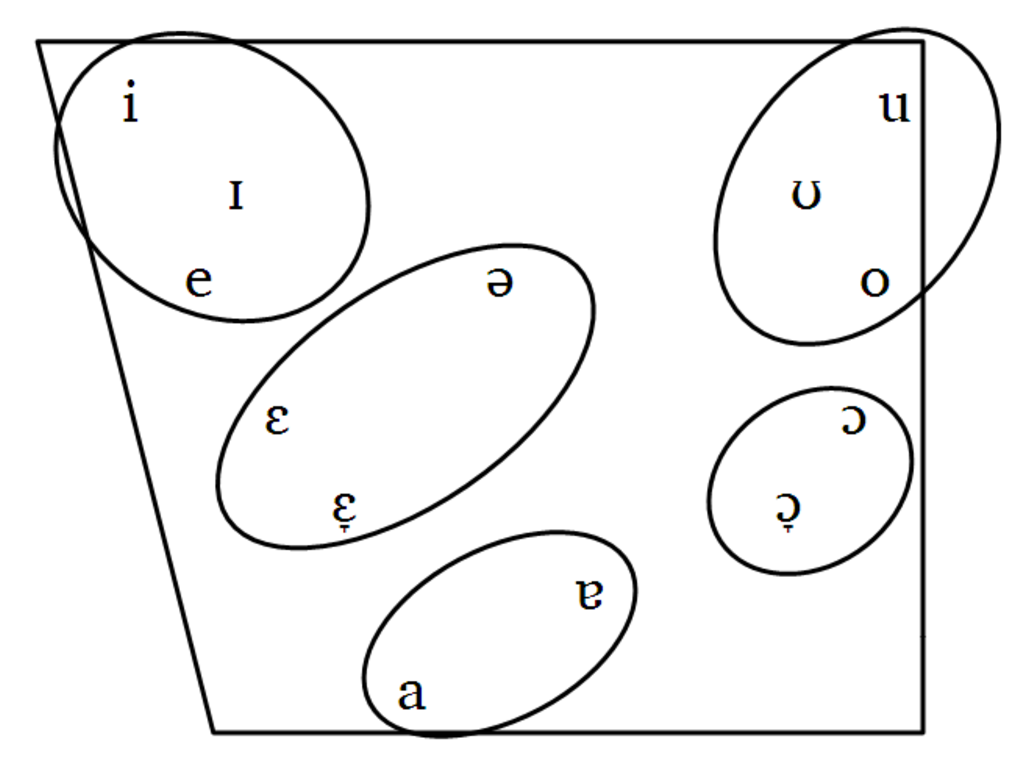
\includegraphics[scale=0.5]{./figures/Figure_2_1}
%\documentclass{article}
%
%\usepackage{tikz}
%\usetikzlibrary{calc}
%\usetikzlibrary{positioning}
%\usetikzlibrary{fit}
%
%\begin{document}

\begin{tikzpicture}[baseline, on grid=true]
\node at (0,0) (ol) {};
\node [right=6cm of ol] (or) {};
\node [below right=4.5cm and 1cm of ol] (ul) {};
\node [below=4.5cm of or] (ur) {};

\draw (ol.center) -- (or.center) -- (ur.center) -- (ul.center) -- (ol.center);

\node[below right=\baselineskip and 0.6cm of ol] (i) {i};
\node[below left=\baselineskip and .25cm of or](u) {u};
\node[below left=\baselineskip and .5cm of u](U) {ʊ};
\node[below right=\baselineskip and .75cm of i] (I) {ɪ};
\node[below right=2\baselineskip and .5cm of i](e) {e};
\node[right=2.25cm of e](E) {ə};
\node[right=2.25cm of E.west](o) {o};
\node[below right=2\baselineskip and .5cm of e](eps) {ε};
\node[right=4cm of eps](oo) {ɔ};
\node[below left=\baselineskip and .5cm of oo](ool) {\textlowering{ɔ}};
\node[below right=\baselineskip and .5cm of eps](epsl) {\textlowering{ε}};

\node[above right=.5\baselineskip and 1.5cm of ul](a) {a};
\node[above right=\baselineskip and 1.25cm of a](A) {ɐ};

\node[draw=black, inner sep=0pt, thick, ellipse, rotate fit=135, fit=(i) (I) (e)] {};
\node[draw=black, inner sep=0pt, thick, ellipse, fit=(u) (U) (o)] {};
\node[draw=black, inner sep=0pt, thick, ellipse, rotate fit=120, fit=(E) (eps) (epsl)] {};
\node[draw=black, inner sep=0pt, thick, ellipse, fit=(a) (A)] {};
\node[draw=black, inner sep=0pt, thick, ellipse, fit=(oo) (ool)] {};


\end{tikzpicture}	
%
%\end{document}
\caption{Vowel space for the Papuan Malay vowels\label{Figure_2.1}}
\end{figure}
 



The phonological processes involved in the allophonic \isi{variation} of the Papuan Malay vowels are discussed in §\ref{Para_2.2.3}.


\subsubsection[Contrast between the vowel segments]{Contrast between the vowel segments\label{Para_2.1.2.2}}

Contrast between the five vowel segments in disyllabic lexical items is presented in minimal or near-minimal pairs in the following tables: in open stressed penultimate syllables in \tabref{Table_2.7}, in closed stressed penultimate syllables in \tabref{Table_2.8}, and in open unstressed ultimate syllables in \tabref{Table_2.9}. When minimal or near-minimal pairs could not be found, another word containing a contrasting vowel segment is given.

\begin{table}
\caption{Vowel contrast in open stressed penultimate syllables\label{Table_2.7}}

\begin{tabular}{llll}

\lsptoprule
 Contrast & Item & Orthogr. & Gloss\\

\midrule
\textstyleChCharisSIL{i{\Tilde}ɛ} & [\textstyleChCharisSIL{ˈi.kʊt̚}] & \textitbf{ikut} & ‘follow’\\
& [\textstyleChCharisSIL{ˈɛ.kɔ̞r}] & \textitbf{ekor} & ‘tail’\\
\textstyleChCharisSIL{i{\Tilde}a} & [\textstyleChCharisSIL{ˈi.ŋɪŋ}] & \textitbf{inging} & ‘wish’\\
& [\textstyleChCharisSIL{ˈa.ŋɪŋ}] & \textitbf{anging} & ‘wind’\\
\textstyleChCharisSIL{i{\Tilde}u} & [\textstyleChCharisSIL{ˈɪ.ɾɪs}] & \textitbf{iris} & ‘cut’\\
& [\textstyleChCharisSIL{ˈʊ.ɾʊs}] & \textitbf{urus} & ‘arrange’\\
\textstyleChCharisSIL{i{\Tilde}ɔ} & [\textstyleChCharisSIL{ˈi.tu}] & \textitbf{itu} & ‘\textsc{d.dist}’\\
& [\textstyleChCharisSIL{ˈɔ.tɔ̞t˺}] & \textitbf{otot} & ‘muscle’\\
\textstyleChCharisSIL{ɛ{\Tilde}a} & [\textstyleChCharisSIL{ˈɛ.dʒɛ̞k̚}] & \textitbf{ejek} & ‘mock’\\
& [\textstyleChCharisSIL{ˈa.dʒɐk}] & \textitbf{ajak} & ‘invite’\\
\textstyleChCharisSIL{ɛ{\Tilde}u} & [\textstyleChCharisSIL{ˈɛ.kɔ̞r}] & \textitbf{ekor} & ‘tail’\\
& [\textstyleChCharisSIL{ˈu.kʊr}] & \textitbf{ukur} & ‘measure’\\
\textstyleChCharisSIL{ɛ{\Tilde}ɔ} & [\textstyleChCharisSIL{ˈɛ.dʒɛ̞k˺}] & \textitbf{ejek} & ‘mock’\\
& [\textstyleChCharisSIL{ˈɔ.dʒɛ̞k˺}] & \textitbf{ojek} & ‘motorbike taxi’\\
\textstyleChCharisSIL{a{\Tilde}u} & [\textstyleChCharisSIL{ˈa.ɾa}] & \textitbf{ara} & ‘direction’\\
& [\textstyleChCharisSIL{ˈu.ɾɐt̚}] & \textitbf{urat} & ‘vein’\\
\textstyleChCharisSIL{u{\Tilde}ɔ} & [\textstyleChCharisSIL{ˈu.dʒʊŋ}] & \textitbf{ujung} & ‘end’\\
& [\textstyleChCharisSIL{ˈɔ.dʒɛ̞k˺}] & \textitbf{ojek} & ‘motorbike taxi’\\
\lspbottomrule
\end{tabular}
\end{table}

\begin{table}
\caption{Vowel contrast in closed stressed penultimate syllables\label{Table_2.8}}

\begin{tabular}{llll}

\lsptoprule
 Contrast & Item & Orthogr. & Gloss\\

\midrule
\textstyleChCharisSIL{i{\Tilde}u} & [\textstyleChCharisSIL{ˈmɪn.ta}] & \textitbf{minta} & ‘request’\\
& [\textstyleChCharisSIL{ˈmʊn.ta}] & \textitbf{munta} & ‘vomit’\\
\textstyleChCharisSIL{i{\Tilde}ɛ} & [\textstyleChCharisSIL{ˈtɪm.bɐŋ}] & \textitbf{timbang} & ‘weigh’\\
& [\textstyleChCharisSIL{ˈtɛ̞m.bɐk̚}] & \textitbf{tembak} & ‘shoot’\\
\textstyleChCharisSIL{i{\Tilde}a} & [\textstyleChCharisSIL{ˈtɪm.ba}] & \textitbf{timba} & ‘fetch’\\
& [\textstyleChCharisSIL{ˈtɐm.ba}] & \textitbf{tamba} & ‘add’\\
\textstyleChCharisSIL{i{\Tilde}ɔ} & [\textstyleChCharisSIL{ˈtɪŋ.kɐt̚}] & \textitbf{tingkat} & ‘level’\\
& [\textstyleChCharisSIL{ˈtɔ̞ŋ.kɐt̚}] & \textitbf{tongkat} & ‘cane’\\
\textstyleChCharisSIL{ɛ{\Tilde}a} & [\textstyleChCharisSIL{ˈsɛ̞n.tu}] & \textitbf{sentu} & ‘touch’\\
& [\textstyleChCharisSIL{ˈsɐn.tɛ}] & \textitbf{sante} & ‘relax’\\
\textstyleChCharisSIL{ɛ{\Tilde}u} & [\textstyleChCharisSIL{ˈtɛ̞m.bɐk̚}] & \textitbf{tembak} & ‘shoot’\\
& [\textstyleChCharisSIL{ˈtʊm.bʊk̚}] & \textitbf{tumbuk} & ‘pound’\\
\textstyleChCharisSIL{ɛ{\Tilde}ɔ} & [\textstyleChCharisSIL{ˈbɛ̞ŋ.kɔ̞k̚}] & \textitbf{bengkok} & ‘be crooked’\\
& [\textstyleChCharisSIL{ˈbɔ̞ŋ.kɔ̞k̚}] & \textitbf{bongkok} & ‘be bent over’\\
\textstyleChCharisSIL{a{\Tilde}u} & [\textstyleChCharisSIL{ˈbɐn.tu}] & \textitbf{bantu} & ‘help’\\
& [\textstyleChCharisSIL{ˈbʊn.tu}] & \textitbf{buntu} & ‘be blocked’\\
\textstyleChCharisSIL{a{\Tilde}ɔ} & [\textstyleChCharisSIL{ˈsɐm.bʊŋ}] & \textitbf{sambung} & ‘continue’\\
& [\textstyleChCharisSIL{ˈsɔ̞m.bɔ̞ŋ}] & \textitbf{sombong} & ‘be arrogant’\\
\textstyleChCharisSIL{u{\Tilde}ɔ} & [\textstyleChCharisSIL{ˈsʊm.bɐŋ}] & \textitbf{sumbang} & ‘donate’\\
& [\textstyleChCharisSIL{ˈsɔ̞m.bɔ̞ŋ}] & \textitbf{sombong} & ‘be arrogant’\\
\lspbottomrule
\end{tabular}
\end{table}

\clearpage

\begin{table}
\caption{Vowel contrast in open unstressed syllables\label{Table_2.9}}

\begin{tabular}{llll}
\lsptoprule
 Contrast & Item & Orthogr. & Gloss\\

\midrule
\textstyleChCharisSIL{i{\Tilde}ɛ} & [\textstyleChCharisSIL{ˈpi.li}] & \textitbf{pili} & ‘choose’\\
& [\textstyleChCharisSIL{ˈpɛ.lɛ}] & \textitbf{pele} & ‘cover’\\
\textstyleChCharisSIL{i{\Tilde}a} & [\textstyleChCharisSIL{ˈka.li}] & \textitbf{kali} & ‘river’\\
& [\textstyleChCharisSIL{ˈka.la}] & \textitbf{kala} & ‘be defeated’\\
\textstyleChCharisSIL{i{\Tilde}u} & [\textstyleChCharisSIL{ˈla.gi}] & \textitbf{lagi} & ‘again’\\
& [\textstyleChCharisSIL{ˈla.gu}] & \textitbf{lagu} & ‘song’\\
\textstyleChCharisSIL{i{\Tilde}ɔ} & [\textstyleChCharisSIL{ˈba.bi}] & \textitbf{babi} & ‘pig’\\
& [\textstyleChCharisSIL{ˈbɔ.bɔ}] & \textitbf{bobo} & ‘palm liquor’\\
\textstyleChCharisSIL{ɛ{\Tilde}u} & [\textstyleChCharisSIL{ˈpa.kɛ}] & \textitbf{pake} & ‘use’\\
& [\textstyleChCharisSIL{ˈpa.ku}] & \textitbf{paku} & ‘nail’\\
\textstyleChCharisSIL{ɛ{\Tilde}ɔ} & [\textstyleChCharisSIL{ˈga.lɛ̞}] & \textitbf{gale} & ‘dig up’\\
& [\textstyleChCharisSIL{ˈga.ɾɔ}] & \textitbf{garo} & ‘scratch’\\
\textstyleChCharisSIL{a{\Tilde}u} & [\textstyleChCharisSIL{ˈbi.sa}] & \textitbf{bisa} & ‘be able’\\
& [\textstyleChCharisSIL{ˈbi.su}] & \textitbf{bisu} & ‘mute’\\
\textstyleChCharisSIL{u{\Tilde}ɔ} & [\textstyleChCharisSIL{ˈtu.bu}] & \textitbf{tubu} & ‘body’\\
& [\textstyleChCharisSIL{ˈtɔ.bɔ}] & \textitbf{tobo} & ‘dive’\\
\lspbottomrule
\end{tabular}
\end{table}

 
\section{Phonological processes\label{Para_2.2}}

In Papuan Malay, two phonological processes are attested for the consonants and one for the vowels: nasal place \isi{assimilation} (§\ref{Para_2.2.1}), tap/trill alternation of the alveolar rhotic (§\ref{Para_2.2.2}), and \isi{centralization} of vowels (§\ref{Para_2.2.3}).


\subsection{Nasal place {assimilation}\label{Para_2.2.1}}
Nasal place \isi{assimilation} applies to nasals as coda in the domain of the prosodic word. While all four nasals occur in the onset position (although velar /\textstyleChCharisSIL{ŋ}/ only occurs in the word-internal onset position), only two nasals occur as coda, namely bilabial /\textstyleChCharisSIL{m}/ and velar /\textstyleChCharisSIL{ŋ}/, as shown in \tabref{Table_2.10}. The velar nasal as a coda assimilates in place of articulation to a following stop or affricate. When preceding the alveolar fricative, the nasal is always realized as velar [\textstyleChCharisSIL{ŋ}], as in \textitbf{bongso} ‘youngest offspring’ or \textitbf{langsung} ‘immediately’. These patterns agree with \citegen[489]{Padgett.1994} cross-linguistic findings that nasals either do “not assimilate in place to fricatives” or that such \isi{assimilation} is, at least, “highly disfavored, while \isi{assimilation} to stops and affricates is pervasive”. (See also \citealt[146--147]{deLacy.2006}; \citealt[554]{Zsiga.2006}; \citealt{Blust.2012}.) An exception to these patterns of nasal \isi{assimilation} is the prefix \textscItal{pe(n)-} ‘\textsc{ag}’ (§\ref{Para_3.1.4}). When preceding the alveolar fricative /s/, the nasal is not realized as alveolar [\textstyleChCharisSIL{n}] but as palatal [\textstyleChCharisSIL{ɲ}], as in \textitbf{penyakit} [\textstyleChCharisSIL{pɛ̞ɲ}–\textstyleChCharisSIL{sakɪt}] ‘disease’, with /\textstyleChCharisSIL{s}/ being deleted (see also \citealt{Blust.2012}; for the \isi{allomorphy} of \textscItal{pe(n)-} see §\ref{Para_3.1.4.1}).


Cross-linguistically, the preservation of the bilabial nasal is not unusual, as \citet[78–207]{deLacy.2006} points out. It is due to the fact, that on the “Place of Articulation” hierarchy, the labial nasal is more marked than the dental or velar ones \citep[129]{deLacy.2006}. Such marked elements “can be specifically targeted for preservation. Consequently, highly marked elements can survive a process that less-marked elements undergo” \citep[146]{deLacy.2006}.\footnote{One anonymous reviewer suggests, however, a different analysis. Given that the nasal in this position obtains its place features from the following segment, not two, but only one nasal phoneme (or ``archiphoneme'') occurs in the word-internal coda position.}

\begin{table}
\caption{Nasal place \isi{assimilation} in the word-internal coda position\label{Table_2.10}}

\begin{tabular}{lllll}
\lsptoprule
 Phoneme & Realization & Item & Orthogr. &  Gloss\\

\midrule
/\textstyleChCharisSIL{m}/ & [\textstyleChCharisSIL{m}] & [\textstyleChCharisSIL{ˈsɪ}\textstyleChCharisSILBlueBold{m}\textstyleChCharisSIL{.}\textstyleChCharisSILBlueBold{p}\textstyleChCharisSIL{ɐŋ}] & \textitbf{simpang} & ‘store’\\
&  & [\textstyleChCharisSIL{kɛ̞}\textstyleChCharisSILBlueBold{m}\textstyleChCharisSIL{.ˈ}\textstyleChCharisSILBlueBold{b}\textstyleChCharisSIL{a.li}] & \textitbf{kembali} & ‘return’\\
/\textstyleChCharisSIL{ŋ}/ & [n] & [\textstyleChCharisSIL{ˈmɪ}\textstyleChCharisSILBlueBold{n}\textstyleChCharisSIL{.}\textstyleChCharisSILBlueBold{t}\textstyleChCharisSIL{a}] & \textitbf{minta} & ‘ask’\\
&  & [\textstyleChCharisSIL{ˈmɐ}\textstyleChCharisSILBlueBold{n}\textstyleChCharisSIL{.}\textstyleChCharisSILBlueBold{d}\textstyleChCharisSIL{i}] & \textitbf{mandi} & ‘bathe’\\
&  & [\textstyleChCharisSIL{ˈhɐ}\textstyleChCharisSILBlueBold{n}\textstyleChCharisSIL{.}\textstyleChCharisSILBlueBold{ʧ}\textstyleChCharisSIL{ʊr}] & \textitbf{hancur} & ‘be shattered’\\
&  & [\textstyleChCharisSIL{ˈɪ}\textstyleChCharisSILBlueBold{n}\textstyleChCharisSIL{.}\textstyleChCharisSILBlueBold{dʒ}\textstyleChCharisSIL{ɐk̚}] & \textitbf{injak} & ‘step on’\\
& [\textstyleChCharisSIL{ŋ}] & [\textstyleChCharisSIL{ˈɐ}\textstyleChCharisSILBlueBold{ŋ}\textstyleChCharisSIL{.}\textstyleChCharisSILBlueBold{k}\textstyleChCharisSIL{ɐt̚}] & \textitbf{angkat} & ‘lift’\\
&  & [\textstyleChCharisSIL{ˈtɪ}\textstyleChCharisSILBlueBold{ŋ}\textstyleChCharisSIL{.}\textstyleChCharisSILBlueBold{g}\textstyleChCharisSIL{i}] & \textitbf{tinggi} & ‘be tall’\\
&  & [\textstyleChCharisSIL{ˈbɔ̞}\textstyleChCharisSILBlueBold{ŋ}\textstyleChCharisSIL{.}\textstyleChCharisSILBlueBold{s}\textstyleChCharisSIL{ɔ̞}] & \textitbf{bongso} & ‘youngest offspring’\\
&  & [\textstyleChCharisSIL{ˈlɐ}\textstyleChCharisSILBlueBold{ŋ}\textstyleChCharisSIL{.}\textstyleChCharisSILBlueBold{s}\textstyleChCharisSIL{ʊŋ}] & \textitbf{langsung} & ‘immediately’\\
\lspbottomrule
\end{tabular}
\end{table}

\largerpage
Nasal place \isi{assimilation} also occurs across word boundaries, when the nasal is in the word-final coda position, as shown in \tabref{Table_2.11}. While bilabial /\textstyleChCharisSIL{m}/ is preserved, velar /\textstyleChCharisSIL{ŋ}/ assimilates in place of articulation to a following stop or affricate, similar to the processes illustrated in \tabref{Table_2.10}. When preceding a fricative-initial or vowel-initial word, or when occurring before a pause or at the end of an utterance, by contrast, the velar nasal is most commonly realized as velar [\textstyleChCharisSIL{ŋ}]. In \tabref{Table_2.11}, this is illustrated with \textitbf{minum} ‘drink’, \textitbf{biking} ‘make’ and \textitbf{bilang} ‘say’. Overall, however, \isi{assimilation} across word boundaries is applied less often than within the prosodic word.

\begin{table}
\caption{Nasal place \isi{assimilation} in the word-final coda position\label{Table_2.11}}

\begin{tabular}{llll}
\lsptoprule
 Phoneme & Item & Orthogr. &  Gloss\\
\midrule
/\textstyleChCharisSIL{m}/ & [\textstyleChCharisSIL{ˈmi.nʊ}\textstyleChCharisSILBlueBold{m}\textstyleChCharisSIL{ ˈ}\textstyleChCharisSILBlueBold{b}\textstyleChCharisSIL{ɔ.bɔ}] & \textitbf{minum bobo} & ‘drink schnapps’\\
& [\textstyleChCharisSIL{ˈmi.nʊ}\textstyleChCharisSILBlueBold{m}\textstyleChCharisSIL{ ˈ}\textstyleChCharisSILBlueBold{d}\textstyleChCharisSIL{u.lu}] & \textitbf{minum dulu} & ‘drink first’\\
& [{\ldots} \textstyleChCharisSIL{ˈmi.nʊ}\textstyleChCharisSILBlueBold{m}\textstyleChCharisSIL{ ˈ}\textstyleChCharisSILBlueBold{k}\textstyleChCharisSIL{i.ˈtɔ̞ŋ}] & \textitbf{{\ldots} minum kitong} & ‘(give) us to drink’\\
& [\textstyleChCharisSIL{ˈmi.nʊ}\textstyleChCharisSILBlueBold{m}\textstyleChCharisSIL{ ˈ}\textstyleChCharisSILBlueBold{i}\textstyleChCharisSIL{.tu}] & \textitbf{minum itu} & ‘drink that’\\
& [\textstyleChCharisSIL{ˈmi.nʊ}\textstyleChCharisSILBlueBold{m}\textstyleChCharisSIL{, ˈ}\textstyleChCharisSILBlueBold{t}\textstyleChCharisSIL{a.pi}] & \textitbf{minum, tapi} & ‘drink, but’\\
/\textstyleChCharisSIL{ŋ}/ & [\textstyleChCharisSIL{ˈbi.kɪ}\textstyleChCharisSILBlueBold{m}\textstyleChCharisSIL{ ˈ}\textstyleChCharisSILBlueBold{b}\textstyleChCharisSIL{a.gʊs}] & \textitbf{biking bagus} & ‘make good’\\
& [\textstyleChCharisSIL{ˈbi.kɪ}\textstyleChCharisSILBlueBold{n}\textstyleChCharisSIL{ ˈ}\textstyleChCharisSILBlueBold{d}\textstyleChCharisSIL{ɪ.a}] & \textitbf{biking dia} & ‘make him/her’\\
& [\textstyleChCharisSIL{ˈbi.kɪ}\textstyleChCharisSILBlueBold{ŋ}\textstyleChCharisSIL{ ˈ}\textstyleChCharisSILBlueBold{k}\textstyleChCharisSIL{ɔ.tɔ̞r}] & \textitbf{biking kotor} & ‘make dirty’\\
& [\textstyleChCharisSIL{ˈbi.kɪ}\textstyleChCharisSILBlueBold{ŋ}\textstyleChCharisSIL{ ˈ}\textstyleChCharisSILBlueBold{s}a] & \textitbf{biking sa} & ‘make me’\\
& [\textstyleChCharisSIL{ˈbi.kɪ}\textstyleChCharisSILBlueBold{ŋ}\textstyleChCharisSIL{ ˈ}\textstyleChCharisSILBlueBold{a}\textstyleChCharisSIL{.pa}] & \textitbf{biking apa} & ‘make what’\\
& [\textstyleChCharisSIL{ˈbi.kɪ}\textstyleChCharisSILBlueBold{ŋ}\textstyleChCharisSIL{, ˈ}\textstyleChCharisSILBlueBold{m}\textstyleChCharisSIL{ɛ.mɐŋ}] & \textitbf{biking, memang} & ‘make, indeed’\\
/\textstyleChCharisSIL{ŋ}/ & [\textstyleChCharisSIL{ˈbi.lɐ}\textstyleChCharisSILBlueBold{m}\textstyleChCharisSIL{ ˈ}\textstyleChCharisSILBlueBold{b}\textstyleChCharisSIL{a.pa}] & \textitbf{bilang bapa} & ‘tell father’\\
& [\textstyleChCharisSIL{ˈbi.lɐ}\textstyleChCharisSILBlueBold{n}\textstyleChCharisSIL{ ˈ}\textstyleChCharisSILBlueBold{d}\textstyleChCharisSIL{ɪ.a}] & \textitbf{bilang dia} & ‘tell him/her’\\
& [\textstyleChCharisSIL{ˈbi.lɐ}\textstyleChCharisSILBlueBold{ŋ}\textstyleChCharisSIL{ ˈ}\textstyleChCharisSILBlueBold{k}\textstyleChCharisSIL{a.ka}] & \textitbf{bilang kaka} & ‘tell older sibling’\\
& [\textstyleChCharisSIL{ˈbi.lɐ}\textstyleChCharisSILBlueBold{ŋ}\textstyleChCharisSIL{ ˈ}\textstyleChCharisSILBlueBold{s}a\textstyleChCharisSIL{.ma}] & \textitbf{bilang sama} & ‘say to’\\
& [\textstyleChCharisSIL{ˈbi.lɐ}\textstyleChCharisSILBlueBold{ŋ}\textstyleChCharisSIL{ ˈ}\textstyleChCharisSILBlueBold{i}\textstyleChCharisSIL{.ni}] & \textitbf{bilang ini} & ‘say this’\\
& [\textstyleChCharisSIL{ˈbi.lɐ}\textstyleChCharisSILBlueBold{ŋ}\textstyleChCharisSIL{, ˈ}\textstyleChCharisSILBlueBold{b}\textstyleChCharisSIL{lʊm}] & \textitbf{bilang, blum} & ‘say, not yet’\\
\lspbottomrule
\end{tabular}
\end{table}

In summary, the data presented in \tabref{Table_2.10} and \tabref{Table_2.11} shows that Papuan Malay has only two underlying nasals in the coda position, namely bilabial /\textstyleChCharisSIL{m}/ and velar /\textstyleChCharisSIL{ŋ}/, with the latter assimilating to a following stop or affricate.

\newpage 

\subsection{Tap/trill alternation of the alveolar rhotic\label{Para_2.2.2}}
The rhotic /r/ is most commonly realized as the voiced alveolar trill [\textstyleChCharisSIL{r}]. In inter-vocalic position, however, the rhotic is realized as the voiced tap [\textstyleChCharisSIL{ɾ}] as illustrated in (\ref{Example_2.1}) and \tabref{Table_2.12}.\footnote{In the examples in this chapter, the first line gives the orthographic representation, while the second lines gives the IPA transcription.} In the C\textsubscript{2} position in CC clusters, the rhotic is also most commonly realized as the voiced trill [r]. The voiced tap, however, is also quite common in this position.

\ea
\label{Example_2.1}
\gll {ta}  { pake}  {\ldots}  {ga\bluebold{ɾ}ɐɐɐm}  {s\bluebold{r}ej}  {\bluebold{r}iʧaaa}  {\ldots}  {dagɪŋ}  {ini}\\
\textsc{1pl}  {take} { }  {salt} {lemongrass}  {red.pepper} {}    {meat}  \textsc{d.prox}\\
\gll {saja}  {asa\bluebold{r}}  dia  {kasi}  {k\bluebold{r}ing}  {di }  {pa\bluebold{r}apa\bluebold{r}a}\\
{\textsc{1sg}}  {smoke}  \textsc{3sg}  {give}  be.dry  {at}  {platform}\\
\glt ‘we used {\ldots} \bluebold{salt}, \bluebold{lemongrass}, \bluebold{red pepper}, {\ldots} this (pig) meat, I \bluebold{smoked} it (and) \bluebold{dried} (it) on a \bluebold{platform}’ \textstyleExampleSource{[080919-004-NP.0037-0038]} \\
\z


\begin{table}
\caption{Tap/trill alternation of rhotic /\textstyleChCharisSIL{r}/\label{Table_2.12}}

\begin{tabular}{llll}
\lsptoprule
 Realization & Item & Orthogr. &  Gloss\\

\midrule

[\textstyleChCharisSIL{r}] & [\textstyleChCharisSIL{ˈ}\textstyleChCharisSILBlueBold{r}\textstyleChCharisSIL{a.kʊs}] & \textitbf{rakus} & ‘be greedy’\\
 & [\textstyleChCharisSIL{ˈk}\textstyleChCharisSILBlueBold{r}\textstyleChCharisSIL{i.ŋɐt̚}] & \textitbf{kringat} & ‘sweat’\\
 & [\textstyleChCharisSIL{ˈmʊ}\textstyleChCharisSILBlueBold{r}\textstyleChCharisSIL{.ni}] & \textitbf{murni} & ‘be pure’\\
 & [\textstyleChCharisSIL{ˈdʒɐŋ.k}\textstyleChCharisSILBlueBold{r}\textstyleChCharisSIL{ɪk̚}] & \textitbf{jangkrik} & ‘cricket’\\
 
[\textstyleChCharisSIL{ɾ}] & [\textstyleChCharisSIL{ˈba.}\textstyleChCharisSILBlueBold{ɾ}\textstyleChCharisSIL{ɐŋ}] & \textitbf{barang} & ‘stuff’\\
 & [\textstyleChCharisSIL{ˈgɔ.}\textstyleChCharisSILBlueBold{ɾ}\textstyleChCharisSIL{ɛ̞ŋ}] & \textitbf{goreng} & ‘fry’\\
 & [\textstyleChCharisSIL{ˈʊ.}\textstyleChCharisSILBlueBold{ɾ}\textstyleChCharisSIL{ʊs}] & \textitbf{urus} & ‘arrange’\\

\lspbottomrule

\end{tabular}
\end{table}

\newpage 
\subsection{Centralization of vowels\label{Para_2.2.3}}
In closed syllables the five vowels are centralized. Close /\textstyleChCharisSIL{i}/ is centralized to [\textstyleChCharisSIL{ɪ}] and /\textstyleChCharisSIL{u}/ to [\textstyleChCharisSIL{ʊ}], open-mid /\textstyleChCharisSIL{ɛ}/ is centralized to [\textstyleChCharisSIL{ɛ̞}] and /\textstyleChCharisSIL{ɔ}/ to [\textstyleChCharisSIL{ɔ̞}], and open /\textstyleChCharisSIL{a}/ is centralized to [\textstyleChCharisSIL{ɐ}], as illustrated in \tabref{Table_2.13}. In unstressed closed syllables with a coda nasal, open-mid /\textstyleChCharisSIL{ɛ}/ can alternatively be centralized to [\textstyleChCharisSIL{ə}] rather than to [\textstyleChCharisSIL{ɛ̞}].

\begin{table}
\caption{Vowel \isi{centralization} in closed syllables\label{Table_2.13}}

\begin{tabular}{cclll}
\lsptoprule
 Phoneme & Realization & \multicolumn{1}{c}{Item} &  \multicolumn{1}{c}{Orthogr.} &   \multicolumn{1}{c}{Gloss}\\


\midrule
/\textstyleChCharisSIL{i}/ & [\textstyleChCharisSIL{ɪ}] & [\textstyleChCharisSIL{ˈt}\textstyleChCharisSILBlueBold{ɪ}\textstyleChCharisSIL{ŋ.gi}] & \textitbf{tinggi} & ‘be high’\\
&  & [\textstyleChCharisSIL{ˈa.d}\textstyleChCharisSILBlueBold{ɪ}\textstyleChCharisSIL{l}] & \textitbf{adil} & ‘be fair’\\
/\textstyleChCharisSIL{u}/ & [\textstyleChCharisSIL{ʊ}] & [\textstyleChCharisSIL{ˈb}\textstyleChCharisSILBlueBold{ʊ}\textstyleChCharisSIL{ŋ.k}\textstyleChCharisSILBlueBold{ʊ}\textstyleChCharisSIL{s}] & \textitbf{bungkus} & ‘pack’\\
&  & [\textstyleChCharisSIL{ˈi.k}\textstyleChCharisSILBlueBold{ʊ}\textstyleChCharisSIL{t̚}] & \textitbf{ikut} & ‘follow’\\
/\textstyleChCharisSIL{ɛ}/ & [\textstyleChCharisSIL{ɛ̞}] & [\textstyleChCharisSIL{ˈg}\textstyleChCharisSILBlueBold{ɛ̞}\textstyleChCharisSIL{n.dɔ̞ŋ}] & \textitbf{gendong} & ‘hold’\\
&  & [\textstyleChCharisSIL{ˈdɔ.ŋ}\textstyleChCharisSILBlueBold{ɛ̞}\textstyleChCharisSIL{ŋ}] & \textitbf{dongeng} & ‘legend’\\
& [\textstyleChCharisSIL{ə}] & [\textstyleChCharisSILBlueBold{ə}\textstyleChCharisSIL{m.ˈpɐt̚}] & \textitbf{empat} & ‘four’\\
&  & [\textstyleChCharisSIL{s}\textstyleChCharisSILBlueBold{ə}\textstyleChCharisSIL{m.ˈbi.lɐŋ}] & \textitbf{sembilang} & ‘nine’\\
/\textstyleChCharisSIL{ɔ}/ & [\textstyleChCharisSIL{ɔ̞}] & [\textstyleChCharisSIL{ˈl}\textstyleChCharisSILBlueBold{ɔ̞}\textstyleChCharisSIL{m.ba}] & \textitbf{lomba} & ‘contest’\\
&  & [\textstyleChCharisSIL{ˈbɛ.l}\textstyleChCharisSILBlueBold{ɔ̞}\textstyleChCharisSIL{k̚}] & \textitbf{belok} & ‘turn’\\
/\textstyleChCharisSIL{a}/ & [\textstyleChCharisSIL{ɐ}] & [\textstyleChCharisSIL{ˈ}\textstyleChCharisSILBlueBold{ɐ}\textstyleChCharisSIL{n.dʒɪŋ}] & \textitbf{anjing} & ‘dog’\\
&  & [\textstyleChCharisSIL{ˈbɪn.t}\textstyleChCharisSILBlueBold{ɐ}\textstyleChCharisSIL{ŋ}] & \textitbf{bintang} & ‘star’\\
\lspbottomrule
\end{tabular}
\end{table}
\section{Phonetic processes\label{Para_2.3}}

In Papuan Malay, a number of phonetic processes occur in addition to the predictable phonological processes described in §\ref{Para_2.2}. These surface phenomena involve unpredict\-able \isi{variation}. For the consonants, the following phenomena are attested: \isi{lenition} of the stops and the voiced affricates as well as \isi{fortition} of the voiceless affricate and the palatal approximant (§\ref{Para_2.3.1.1}), \isi{elision} of the voiceless stops, the alveolar fricative, the velar nasal, and the liquids (§\ref{Para_2.3.1.2}), and \isi{devoicing} of the alveolar rhotic (§\ref{Para_2.3.1.3}). The vowels can undergo the following phonetic processes: \isi{centralization} and \isi{lowering} (§\ref{Para_2.3.2.1}), \isi{nasalization} (§\ref{Para_2.3.2.2}), and \isi{lengthening} (§\ref{Para_2.3.2.3}). In addition, this section includes a discussion on alternative realizations of the VC sequences /\textstyleChCharisSIL{aj}/ and /\textstyleChCharisSIL{aw}/ (§\ref{Para_2.3.3})


\subsection{Phonetic processes for consonants\label{Para_2.3.1}}
\subsubsection[Lenition and {fortition}]{Lenition and {fortition}\label{Para_2.3.1.1}}
 
Lenition, or weakening, is attested for the stops and affricates and can occur in word-internal inter-vocalic position, and word-initial position. Fortition, or strengthening, occurs very rarely and is only attested for the voiceless affricate and the palatal approximant as word-initial onset.


Most of the stops and the voiced affricate can also be lenited in word-initial position when following a word with final vowel. In this environment, however, \isi{lenition} of the voiced affricate occurs less often than \isi{lenition} of the stops. Inter-vocalically across word-boundaries, the word-initial obstruents are lenited to the same fricatives as word-internally, as shown in \tabref{Table_2.15}. Also, /\textstyleChCharisSIL{p}/ can be lenited to [\textstyleChCharisSIL{f}], and /\textstyleChCharisSIL{d}/ and /\textstyleChCharisSIL{d}\textstyleChCharisSIL{ʒ}/ can be lenited to [\textstyleChCharisSIL{j}]. Word-initial \isi{lenition} to a fricative is also attested for /\textstyleChCharisSIL{b}/, /\textstyleChCharisSIL{d}/, and /\textstyleChCharisSIL{k}/ when following a nasal. In this environment, /\textstyleChCharisSIL{d}/ can also be lenited to [\textstyleChCharisSIL{n}]. Again, \isi{lenition} to a fricative is unattested for the voiceless alveolar and palato-alveolar segments. Likewise, \isi{lenition} in word-initial position is unattested for /\textstyleChCharisSIL{g}/.\footnote{One lexical item in particular undergoes \isi{lenition} of its word-initial stop: the long and the short forms of the third person singular \isi{pronoun}, \textitbf{dia}/\textitbf{de} ‘\textsc{3sg}’. Onset /\textstyleChCharisSILviiivpt{d}/ can be lenited to [\textstyleChCharisSILviiivpt{j}] when following a lexical item with a voiceless stop, the alveolar fricative /\textstyleChCharisSILviiivpt{s}/, or the rhotic /\textstyleChCharisSILviiivpt{r}/ in word-final coda position.}



\begin{table} 
\caption{Lenition of stops and affricates in word-internal inter-vocalic position\label{Table_2.14}}

\begin{tabular}{clll}
\lsptoprule
 Phoneme &  \multicolumn{1}{c}{Item} &  \multicolumn{1}{c}{Orthogr.} &   \multicolumn{1}{c}{Gloss}\\

\midrule
/\textstyleChCharisSIL{p}/ & [\textstyleChCharisSIL{ˈba.}\textstyleChCharisSILBlueBold{ɸ}\textstyleChCharisSIL{a}] & \textitbf{bapa} & ‘father’\\
/\textstyleChCharisSIL{b}/ & [\textstyleChCharisSIL{ˈsa.}\textstyleChCharisSILBlueBold{β}\textstyleChCharisSIL{ɐr}] & \textitbf{sabar} & ‘be patient’\\
/\textstyleChCharisSIL{d}/ & [\textstyleChCharisSIL{ˈsʊ.}\textstyleChCharisSILBlueBold{ð}\textstyleChCharisSIL{a}] & \textitbf{suda} & ‘already’\\
/\textstyleChCharisSIL{k}/ & [\textstyleChCharisSIL{ˈma.}\textstyleChCharisSILBlueBold{x}\textstyleChCharisSIL{ɐŋ}] & \textitbf{makang} & ‘eat’\\
/\textstyleChCharisSIL{g}/ & [\textstyleChCharisSIL{ˈba.}\textstyleChCharisSILBlueBold{ɣ}\textstyleChCharisSIL{i}] & \textitbf{bagi} & ‘divide’\\
/\textstyleChCharisSIL{d}\textstyleChCharisSIL{ʒ}/ & [\textstyleChCharisSIL{ˈsa.}\textstyleChCharisSILBlueBold{ʝ}\textstyleChCharisSIL{a}] & \textitbf{saja} & ‘just’\\
/\textstyleChCharisSIL{t}\textstyleChCharisSIL{ʃ}/ & [\textstyleChCharisSIL{ˈpa.}\textstyleChCharisSILBlueBold{j}\textstyleChCharisSIL{ɛ}] & \textitbf{pace} & ‘man’\\
\lspbottomrule
\end{tabular}
\end{table}



Inter-vocalically, the stops and the voiced affricate can be lenited by means of spirantization to fricatives, as illustrated in \tabref{Table_2.14}: /\textstyleChCharisSIL{p}/ is lenited to [\textstyleChCharisSIL{ɸ}], /\textstyleChCharisSIL{b}/ to [\textstyleChCharisSIL{β}], /\textstyleChCharisSIL{d}/ to [\textstyleChCharisSIL{ð}], /\textstyleChCharisSIL{k}/ to [\textstyleChCharisSIL{x}], /\textstyleChCharisSIL{g}/ to [\textstyleChCharisSIL{ɣ}], and /\textstyleChCharisSIL{d}\textstyleChCharisSIL{ʒ}/ to [\textstyleChCharisSIL{ʝ}]. This process is unattested, however, for the voiceless alveolar and palato-alveolar segments. The voiceless affricate /\textstyleChCharisSIL{t}\textstyleChCharisSIL{ʃ}/ can be lenited to the palatal approximant [\textstyleChCharisSIL{j}], while \isi{lenition} of alveolar /\textstyleChCharisSIL{t}/ is unattested.




\begin{table}[t] 
\caption{Lenition of stops and affricates in word-initial position\label{Table_2.15}}


\begin{tabular}{clll}
\lsptoprule
 Phoneme &  \multicolumn{1}{c}{Item} &  \multicolumn{1}{c}{Orthogr.} &   \multicolumn{1}{c}{Gloss}\\

\midrule
/\textstyleChCharisSIL{p}/ & [\textstyleChCharisSIL{ˈdɛ }\textstyleChCharisSILBlueBold{ɸ}\textstyleChCharisSIL{u}] & \textitbf{de pu} & ‘his (grandson)’\\
&  & \textsc{3sg} \textsc{poss} & \\
& [\textstyleChCharisSIL{ˈdi.a ˈ}\textstyleChCharisSILBlueBold{f}\textstyleChCharisSIL{luŋ.ku}] & \textitbf{dia palungku} & ‘he punched’\\
&  & \textsc{3sg} punch & \\

/\textstyleChCharisSIL{b}/ & [\textstyleChCharisSIL{ˈjɛ ˈ}\textstyleChCharisSILBlueBold{β}\textstyleChCharisSIL{i.lɐŋ}] & \textitbf{de bilang} & ‘he/she said’\\
&  & \textsc{3sg} say & \\
& [\textstyleChCharisSIL{ˈdʒa.rɪm ˈ}\textstyleChCharisSILBlueBold{β}\textstyleChCharisSIL{ɔ.lɛ}] & \textitbf{jaring bole} & (the) net (is) permitted\\
&  & net may & \\

/\textstyleChCharisSIL{d}/ & [\textstyleChCharisSIL{mˈla, ɛ ˈ}\textstyleChCharisSILBlueBold{ð}\textstyleChCharisSIL{ɛ̞p̚}] & \textitbf{mulay, eh dep} & ‘(he) started, uh his’\\
&  & start uh \textsc{3sg:poss} & \\
& [\textstyleChCharisSIL{ˈsa.dʒa }\textstyleChCharisSILBlueBold{j}\textstyleChCharisSIL{ɛ̞.ˈŋɐŋ}] & \textitbf{saja dengang} & ‘just with’\\
&  & just with & \\
& [\textstyleChCharisSIL{ˈspʊl ˈba.ðɐn ˈ}\textstyleChCharisSILBlueBold{ð}\textstyleChCharisSIL{i}] & \textitbf{spul badang di} & ‘wash (your) body in’\\
&  & wash body at & \\
& [\textstyleChCharisSIL{ˈki.tɔ̞n ˈ}\textstyleChCharisSILBlueBold{n}\textstyleChCharisSIL{u.a}] & \textitbf{kitong dua} & ‘we two’\\
&  & \textsc{1pl} two & \\

/\textstyleChCharisSIL{k}/ & [\textstyleChCharisSIL{ˈa.dɛ̞.ˈ}\textstyleChCharisSILBlueBold{x}\textstyleChCharisSIL{a.xa}] & \textitbf{ade-kaka} & ‘siblings’\\
&  & ySb oSb & \\
& [\textstyleChCharisSIL{dɛ̞.ˈŋɐŋ ˈ}\textstyleChCharisSILBlueBold{x}\textstyleChCharisSIL{a.xa}] & \textitbf{dengang kaka} & ‘with (the) older sibling’\\
&  & with oSb & \\

/\textstyleChCharisSIL{d}\textstyleChCharisSIL{ʒ}/ & [\textstyleChCharisSIL{ˈsa pu ˈ}\textstyleChCharisSILBlueBold{ʝ}\textstyleChCharisSIL{ɛ̞.kɛ̞t˺}] & \textitbf{sa pu jeket} & ‘my jacket’\\
&  & 1\textsc{sg} \textsc{poss} jacket & \\
& [\textstyleChCharisSIL{{\ldots} ˈi.tu, ˈ}\textstyleChCharisSILBlueBold{j}\textstyleChCharisSIL{a.ŋɐŋ}] & \textitbf{{\ldots} itu, jangang} & ‘those (big ones), don’t’\\
&  & \textsc{d.dist} \textsc{neg.imp} & \\
\lspbottomrule
\end{tabular}
\end{table}





  
Fortition occurs very rarely and is attested only for the voiceless affricate and the palatal approximant in word-initial position. In the more thoroughly transcribed 150-minute extract of the corpus, \isi{fortition} of /\textstyleChCharisSIL{t}\textstyleChCharisSIL{ʃ}/ is attested once and strengthening of /\textstyleChCharisSIL{j}/ twice, as shown in \tabref{Table_2.16}.

\begin{table}[p]
\caption{ Fortition of the voiceless affricate and the voiced palatal approximant\label{Table_2.16}}
\begin{tabular}{clll}
\lsptoprule
Phoneme &  \multicolumn{1}{c}{Item} &  \multicolumn{1}{c}{Orthogr.} &   \multicolumn{1}{c}{Gloss}\\
\midrule
/\textstyleChCharisSIL{ʧ}/ & [\textstyleChCharisSIL{ˈdɛ̞p˺} \textstyleChCharisSILBlueBold{ˈt}\textstyleChCharisSIL{u.ʧu}] & \textitbf{de pu cucu} & ‘his grandchild’\\
&  & \textsc{3sg} \textsc{poss} grandchild & \\

/\textstyleChCharisSIL{j} / & [\textstyleChCharisSIL{ˈej} \textstyleChCharisSILBlueBold{ˈdʒ}\textstyleChCharisSIL{ɐŋ bɛ.}ˌ\textstyleChCharisSIL{sɐr{\Tilde}bɛ.ˈsɐr}] & \textitbf{ey yang {besar{\Tilde}besar}} & ‘hey those big ones’\\
&  & hey \textsc{rel} \textsc{rdp} {\Tilde}be.big & \\
& [\textstyleChCharisSIL{ˈ}\textstyleChCharisSILBlueBold{ʝ}\textstyleChCharisSIL{a}] & \textitbf{yo} & ‘yes’\footnote{Affirmative \textitbf{yo} ‘yes’ is frequently realized as \textitbf{ya} (see §\ref{Para_5.4.3}).}\\
&  & yes & \\
\lspbottomrule
\end{tabular}
\end{table}



\subsubsection[Elision]{Elision\label{Para_2.3.1.2}}
 
Elision of a word-final segment is attested for the voiceless stops, the alveolar fricative, the velar nasal, and both liquids, as shown in \tabref{Table_2.17}. Concerning the voiceless stops, \isi{elision} applies most frequently to /\textstyleChCharisSIL{k}/. Elision of /\textstyleChCharisSIL{t}/ occurs less frequently and is unattested for /\textstyleChCharisSIL{p}/. Word-final /\textstyleChCharisSIL{s}/ is much less prone to \isi{elision} than word-final stops, with the corpus containing only two lexical items with deleted /\textstyleChCharisSIL{s}/. When the word-final velar nasal is omitted, it is always realized as \isi{nasalization} on the preceding vowel.\footnote{More in-depth acoustic phonetic analysis is needed to determine whether the nasalized vowels remain centralized. Since these vowels occur in open syllables they are represented as their non-centralized allophones (for more details see §\ref{Para_2.2.3}) pending further results.} Elision of the liquids occurs only very rarely. The exception is \textitbf{ambil} ‘fetch’. Of its 221 tokens, 49 tokens are realized without word-final /\textstyleChCharisSIL{l}/: [\textstyleChCharisSIL{ˈɐm.bi}] (48 tokens) and [\textstyleChCharisSIL{ˈɐm.be.a}] (1 token).

\begin{table}
\caption[Elision of the voiceless stops\ldots]{Elision of the voiceless stops, the alveolar fricative, the velar nasal, and the liquids in word-final position\label{Table_2.17}}

\begin{tabular}{clll}
\lsptoprule
 Phoneme &  \multicolumn{1}{c}{Item} &  \multicolumn{1}{c}{Orthogr.} &   \multicolumn{1}{c}{Gloss}\\
\midrule

/\textstyleChCharisSIL{t}/ & [\textstyleChCharisSIL{ˈsa.ki}] & \textitbf{sakit} & ‘be sick’\\
/\textstyleChCharisSIL{k}/ & [\textstyleChCharisSIL{ˈma.sa}] & \textitbf{masak} & ‘cook’\\
/\textstyleChCharisSIL{s}/ & [\textstyleChCharisSIL{ˈtru}] & \textitbf{trus} & ‘be continuous’\\
/\textstyleChCharisSIL{ŋ}/ & [\textstyleChCharisSIL{ˈɐn.dʒ\~{i}}] & \textitbf{anjing} & ‘dog’\\
/\textstyleChCharisSIL{r}/ & [\textstyleChCharisSIL{ˈla.pa}] & \textitbf{lapar} & ‘be hungry’\\
/\textstyleChCharisSIL{l}/ & [\textstyleChCharisSIL{ˈɐm.bi} / \textstyleChCharisSIL{ˈɐm.be.a}] & \textitbf{ambil} & ‘fetch’\\

\lspbottomrule
\end{tabular}
\end{table}
\subsubsection[Devoicing]{Devoicing\label{Para_2.3.1.3}}

Devoicing applies only to the rhotic trill as word-final coda. In this position, it is most commonly realized as [\textstyleChCharisSIL{r}]. Before a pause or in utterance-final position, however, the trill can also be devoiced to [\textstyleChCharisSIL{r̥}], as illustrated in (\ref{Example_2.2}).


\ea
\label{Example_2.2}
\gll \bluebold{skaɾɐn}  dɔ̞ŋ  kasi  dɪa  \bluebold{sɛ̞ntɛ̞r̥},  kasi  \bluebold{sɛ̞ntɛ̞r}  dɔ̞ŋ  kasi {\ldots}\\
now  \textsc{3pl}  give  \textsc{3sg}  flashlight  give  flashlight  \textsc{3pl}  give {}\\
\glt
‘\bluebold{now} they give him a \bluebold{flashlight}, (having) given (him) a \bluebold{flashlight} they give (him) \ldots’ \textstyleExampleSource{[081108-003-JR.0002]}\\
\z

\subsubsection[Palatalization]{Palatalization\label{Para_2.3.1.4}}

Palatalization of /\textstyleChCharisSIL{s}/ is rare. It occurs only in lexical roots with a /\textstyleChCharisSIL{si.}V/ sequence, if this root has three or more syllables and if the syllable containing /s/ is unstressed. The \isi{palatalization} of /\textstyleChCharisSIL{s}/ co-occurs with the \isi{elision} of the close front vowel /\textstyleChCharisSIL{i}/, which reduces the number of syllables by one, as illustrated in \tabref{Table_2.18}. Hence, /\textstyleChCharisSIL{si.}V/ is realized as [\textstyleChCharisSIL{sʲ}V]. Attested is one polysyllabic \isi{lexical root} with a /\textstyleChCharisSIL{si.}V/ sequence, the high frequency item \textitbf{siapa} ‘who’. In lexical roots with a /\textstyleChCharisSIL{si.}V/ sequence in which the syllable containing /s/ is stressed, \isi{palatalization} of the fricative is unattested. Attested are the three lexical roots listed in \tabref{Table_2.18}, all of which are disyllabic: \textitbf{sial} ‘be unfortunate’, \textitbf{siang} ‘midday’, and \textitbf{siap} ‘be ready’.


This lack of \isi{assimilation} in stressed syllables does, however, also apply to lexical items with more than two syllables, as evidenced by three polysyllabic loanwords, presented in §\ref{Para_2.5.2.3}. The occurrence of /\textstyleChCharisSIL{s}/ in a /\textstyleChCharisSIL{si.}V/ sequence together with the \isi{stress pattern} of the respective lexical item does not, however, \isi{condition} the \isi{palatalization} of the fricative. This is evidenced by the fact that \textitbf{siapa} ‘who’ is realized quite commonly without \isi{palatalization}: [\textstyleChCharisSIL{ˈsa.pa}].



The frequency counts in \tabref{Table_2.18} are based on the broad transcription of the entire 16-hour corpus (16-\textsc{h-c}) and the more thoroughly transcribed 150-minute extract (150-\textsc{m-c}).\footnote{The broad transcription of the 16-hour corpus makes no distinction between the unpalatalized and the palatalized realizations of \textitbf{siapa} ‘who’, [\textstyleChCharisSILviiivpt{si.ˈa.pa}] and [\textstyleChCharisSILviiivpt{ˈsʲa.pa}], respectively. Hence, a more thorough transcription of all 196 /\textstyleChCharisSILviiivpt{siapa}/ tokens is required to establish whether speakers sometimes realize the \isi{interrogative} as the trisyllabic item [\textstyleChCharisSILviiivpt{si.ˈa.pa}] or whether they always palatalize the fricative and thereby realize the item as disyllabic [\textstyleChCharisSILviiivpt{ˈsʲa.pa}]. In the more thoroughly transcribed 150-minute extract of the corpus the trisyllabic \textitbf{siapa} [\textstyleChCharisSILviiivpt{si.ˈa.pa}] ‘who’ is unattested.}

\begin{table}
\caption{Palatalization of the alveolar fricative in loanwords\label{Table_2.18}}

\begin{tabularx}{\textwidth}{lp{1.2cm}p{2.5cm}Xrr}
\lsptoprule
 \multicolumn{1}{c}{Stress} & \multicolumn{1}{c}{Orthogr.} & \multicolumn{1}{c}{Gloss} & \multicolumn{1}{c}{Realization} & \multicolumn{1}{c}{Freq.} &  \multicolumn{1}{c}{Freq.}\\
&  &  &  & 16-\textsc{h-c} &  150-\textsc{m-c}\\

\midrule
/\textstyleChCharisSIL{si}/ unstressed & \textitbf{siapa} & ‘who’ & [\textstyleChCharisSILBlueBold{si.ˈa}\textstyleChCharisSIL{.pa}] &  196 &  {}-{}-{}-\\
&  &  & [\textstyleChCharisSIL{ˈ}\textstyleChCharisSILBlueBold{sʲa}\textstyleChCharisSIL{.pa}] &  {}-{}-{}- &  40\\
&  &  & [\textstyleChCharisSIL{ˈ}\textstyleChCharisSILBlueBold{sa}\textstyleChCharisSIL{.pa}] &  115 &  10\\
/\textstyleChCharisSIL{ˈsi}/ stressed & \textitbf{sial} & ‘be unfortunate’ & [\textstyleChCharisSIL{ˈ}\textstyleChCharisSILBlueBold{si.ɐ}\textstyleChCharisSIL{l}] &  1 &  1\\
& \textitbf{siang} & ‘midday’ & [\textstyleChCharisSIL{ˈ}\textstyleChCharisSILBlueBold{si.ɐ}\textstyleChCharisSIL{ŋ}] &  55 &  6\\
& \textitbf{siap} & ‘be ready’ & [\textstyleChCharisSIL{ˈ}\textstyleChCharisSILBlueBold{si.ɐ}\textstyleChCharisSIL{p̚}] &  54 &  2\\
\lspbottomrule
\end{tabularx}
\end{table}
\subsection{Phonetic processes for vowels\label{Para_2.3.2}}
\subsubsection[Centralization and {lowering}]{Centralization and {lowering}\label{Para_2.3.2.1}}

In addition to the regular de\isi{centralization} of the vowels in closed syllables, the data indicates two environments where \isi{centralization} of vowels occurs on an irregular basis in open syllables: (1) under the influence of central vowel /\textstyleChCharisSIL{a}/, and (2) under the influence of the corresponding centralized allophone occurring in closed syllables. In addition, the close vowels are very commonly lowered in fast speech.


In open syllables, the close and open-mid vowels are frequently centralized under the influence of the central vowel /\textstyleChCharisSIL{a}/, similar to the process of \isi{centralization} in closed syllables (§\ref{Para_2.2.3}) In unstressed open syllables, open-mid /\textstyleChCharisSIL{ɛ}/ can alternatively be centralized to [\textstyleChCharisSIL{ə}] rather than to [\textstyleChCharisSIL{ɛ̞}].

\begin{table}
\caption{Vowel \isi{centralization} under the influence of central vowel /\textstyleChCharisSIL{a}/\label{Table_2.19}}

\begin{tabular}{cllll}
\lsptoprule
 Phoneme & Realization & \multicolumn{1}{c}{Item} & \multicolumn{1}{c}{Orthogr.} &  \multicolumn{1}{c}{Gloss}\\

\midrule
/\textstyleChCharisSIL{i}/ & [\textstyleChCharisSIL{ɪ}] & [\textstyleChCharisSIL{ˈd}\textstyleChCharisSILBlueBold{ɪ}\textstyleChCharisSIL{.a}] & \textitbf{dia} & ‘\textsc{3sg}’\\
&  & [\textstyleChCharisSIL{ˈh}\textstyleChCharisSILBlueBold{ɪ}\textstyleChCharisSIL{.lɐŋ}] & \textitbf{hilang} & ‘be lost’\\
/\textstyleChCharisSIL{u}/ & [\textstyleChCharisSIL{ʊ}] & [\textstyleChCharisSIL{ˈl}\textstyleChCharisSILBlueBold{ʊ}\textstyleChCharisSIL{.ɐs}] & \textitbf{luas} & ‘be vast’\\
&  & [\textstyleChCharisSIL{ˈb}\textstyleChCharisSILBlueBold{ʊ}\textstyleChCharisSIL{.kɐŋ}] & \textitbf{bukang} & ‘\textsc{neg}’\\
/\textstyleChCharisSIL{ɛ}/ & [\textstyleChCharisSIL{ɛ̞}] & [\textstyleChCharisSIL{ˈb}\textstyleChCharisSILBlueBold{ɛ̞}\textstyleChCharisSIL{.ɾa}] & \textitbf{bera} & ‘defecate’\\
&  & [\textstyleChCharisSIL{ˈh}\textstyleChCharisSILBlueBold{ɛ̞}\textstyleChCharisSIL{.la}] & \textitbf{hela} & ‘haul’\\
& [\textstyleChCharisSIL{ə}] & [\textstyleChCharisSIL{b}\textstyleChCharisSILBlueBold{ə}\textstyleChCharisSIL{.ˈkɐs}] & \textitbf{bekas} & ‘trace’\\
&  & [\textstyleChCharisSIL{l}\textstyleChCharisSILBlueBold{ə}\textstyleChCharisSIL{.ˈpɐs}] & \textitbf{lepas} & ‘free’\\
/\textstyleChCharisSIL{ɔ}/ & [\textstyleChCharisSIL{ɔ̞}] & [\textstyleChCharisSIL{ˈh}\textstyleChCharisSILBlueBold{ɔ̞}\textstyleChCharisSIL{.sa}] & \textitbf{hosa} & ‘pant’\\
&  & [\textstyleChCharisSIL{ˈk}\textstyleChCharisSILBlueBold{ɔ̞}\textstyleChCharisSIL{.lɐm}] & \textitbf{kolam} & ‘big hole’\\
\lspbottomrule
\end{tabular}
\end{table}

In open syllables, the close and open-mid vowels can also be centralized under the influence of the corresponding centralized allophone occurring in a closed syllable, as illustrated in \tabref{Table_2.20} (see also §\ref{Para_2.2.3}).

\begin{table} 

\caption[Vowel \isi{centralization} harmony]{Vowel \isi{centralization} harmony\label{Table_2.20}\footnote{The following lexemes are loanwords: \textitbf{propinsi} ‘province’ and \textitbf{skripsi} ‘minithesis’. The following lexemes are \isi{historically derived} by (unproductive) \isi{affixation}: \textitbf{bertemu} ‘be friends’, \textitbf{berkebung} ‘farm’, and \textitbf{meleset} ‘miss a target’.}}

\begin{tabularx}{\textwidth}{cp{3cm}p{2cm}p{2cm}p{2.5cm}}
\lsptoprule
 Phoneme & \multicolumn{1}{c}{Environment} & \multicolumn{1}{c}{Item} & \multicolumn{1}{c}{Orthogr.} &  \multicolumn{1}{c}{Gloss}\\

\midrule
/\textstyleChCharisSIL{i}/ & \multirow{2}{3cm}{[\textstyleChCharisSIL{ɪ}] in open \textsc{sylb} preceded by [\textstyleChCharisSIL{ɪ}C]} & [\textstyleChCharisSIL{prɔ.ˈpɪn.s}\textstyleChCharisSILBlueBold{ɪ}]   & \textitbf{propinsi} & ‘province’\\

   & & [\textstyleChCharisSIL{ˈskrɪp̚.s}\textstyleChCharisSILBlueBold{ɪ}] & \textitbf{skripsi} & ‘minithesis’\\
 & \multirow{2}{3cm}{[\textstyleChCharisSIL{ɪ}] in open \textsc{sylb} followed by [\textstyleChCharisSIL{ɪ}C]} & [\textstyleChCharisSIL{ˈm}\textstyleChCharisSILBlueBold{ɪ}\textstyleChCharisSIL{.ɾɪŋ}] & \textitbf{miring} & ‘be sideways’\\
 & & [\textstyleChCharisSIL{ˈg}\textstyleChCharisSILBlueBold{ɪ}\textstyleChCharisSIL{.lɪŋ}] & \textitbf{giling} & ‘grind’\\
/\textstyleChCharisSIL{u}/ & \multirow{2}{3cm}{[\textstyleChCharisSIL{ʊ}] in open \textsc{sylb} preceded by [\textstyleChCharisSIL{ʊ}C]} & [\textstyleChCharisSIL{ˈbʊm.b}\textstyleChCharisSILBlueBold{ʊ}] & \textitbf{bumbu} & ‘bamboo’\\
  & & [\textstyleChCharisSIL{ˈbʊn.t}\textstyleChCharisSILBlueBold{ʊ}] & \textitbf{buntu} & ‘be blocked’\\
& \multirow{2}{3cm}{[\textstyleChCharisSIL{ʊ}] in open \textsc{sylb} followed by [\textstyleChCharisSIL{ʊ}C]} & [\textstyleChCharisSIL{ˈl}\textstyleChCharisSILBlueBold{ʊ}\textstyleChCharisSIL{.ɾʊs}] & \textitbf{lurus} & ‘be straight’\\
 & & [\textstyleChCharisSIL{ˈt}\textstyleChCharisSILBlueBold{ʊ}\textstyleChCharisSIL{.ɾʊŋ}] & \textitbf{turung} & ‘descend’\\
/\textstyleChCharisSIL{ɛ}/ & \multirow{2}{3cm}{[\textstyleChCharisSIL{ɛ̞}] in open \textsc{sylb} preceded by [\textstyleChCharisSIL{ɛ̞}C]} & [\textstyleChCharisSIL{bɛ̞r.ˈt}\textstyleChCharisSILBlueBold{ɛ̞}\textstyleChCharisSIL{.mu}] & \textitbf{bertemu} & ‘be friends’\\
&  & [\textstyleChCharisSIL{ˌbɛ̞r.k}\textstyleChCharisSILBlueBold{ɛ̞}\textstyleChCharisSIL{.ˈbʊŋ}] & \textitbf{berkebung} & ‘do farming’\\
& \multirow{2}{3cm}{[\textstyleChCharisSIL{ɛ̞}] in open \textsc{sylb} followed by [\textstyleChCharisSIL{ɛ̞}C]} & [\textstyleChCharisSIL{ˈ}\textstyleChCharisSILBlueBold{ɛ̞}\textstyleChCharisSIL{.pɛ̞ŋ}] & \textitbf{epeng} & ‘important’\\
 & & [\textstyleChCharisSIL{mɛ.ˈl}\textstyleChCharisSILBlueBold{ɛ̞}\textstyleChCharisSIL{.sɛ̞t̚}] & \textitbf{meleset} & ‘miss a target’\\
/\textstyleChCharisSIL{ɔ}/ &\multirow{2}{3cm}{[\textstyleChCharisSIL{ɔ̞}] in open \textsc{sylb} preceded by [\textstyleChCharisSIL{ɔ̞}C]} & [\textstyleChCharisSIL{ˈbɔ̞ŋ.s}\textstyleChCharisSILBlueBold{ɔ̞}] & \textitbf{bongso} & ‘youngest child’\\
&  & [\textstyleChCharisSIL{ˈʧɔ̞n.t}\textstyleChCharisSILBlueBold{ɔ̞}] & \textitbf{conto} & ‘example’\\
& \multirow{2}{3cm}{[\textstyleChCharisSIL{ɔ̞}] in open \textsc{sylb} followed by [\textstyleChCharisSIL{ɔ̞}C]} & [\textstyleChCharisSIL{ˈr}\textstyleChCharisSILBlueBold{ɔ̞}\textstyleChCharisSIL{.kɔ̞k̚}] & \textitbf{rokok} & ‘cigarette’\\
& & [\textstyleChCharisSIL{ˈk}\textstyleChCharisSILBlueBold{ɔ̞}\textstyleChCharisSIL{.dɔ̞k̚}] & \textitbf{kodok} & ‘frog’\\

\lspbottomrule
\end{tabularx}

\end{table}

In fast speech, the close vowels /\textstyleChCharisSIL{i}/ and /\textstyleChCharisSIL{u}/ are very commonly lowered and realized as the close-mid vowels [\textstyleChCharisSIL{e}] and [\textstyleChCharisSIL{o}] respectively, as demonstrated in (\ref{Example_2.3}) to (\ref{Example_2.6}). In (\ref{Example_2.3}) the \isi{verb} \textitbf{kasi} ‘give’ is realized as [\textstyleChCharisSIL{ˈka.se}], and in (\ref{Example_2.4}) the \isi{verb} \textitbf{balik} ‘turn around’ is realized as [\textstyleChCharisSIL{ˈba.le}].\footnote{Concerning the \isi{elision} of the word-final stop see §\ref{Para_2.3.1.2}.} In (\ref{Example_2.5}) the \isi{numeral} \textitbf{dua} ‘two’ is realized as [\textstyleChCharisSIL{ˈdo.a}] and in (\ref{Example_2.6}) the common \isi{noun} \textitbf{lubang} ‘hole’ is realized as [\textstyleChCharisSIL{ˈlo.bɐŋ}]



\ea
\label{Example_2.3}
\gll  {\ldots}  mɔ  bikɪn  papɛda  mɔ  \bluebold{kase}  anana  makɐn\\
  {} want  \textsc{3pl}  sagu.porridge  want  give  \textsc{rdp}{\Tilde}child  eat\\
\glt 
‘[they said (they) wanted to catch chickens and then] (they) wanted to make sagu porridge to \bluebold{give} the children to eat’ \textstyleExampleSource{[081010-001-Cv.0191]}
\z

\ea
\label{Example_2.4}
\gll  itu  Bɔp  Bɔp  itu,  de  biasa  \bluebold{bale}\\
\textsc{d.dist}  Bop  Bop  \textsc{d.dist}  \textsc{3sg}  be.usual  turn.around\\
\glt 
‘that was Bob, that Bob, he usually \bluebold{(flies) a circle}’ (Lit. ‘turns around’) \textstyleExampleSource{[081011-010-Cv.0019]}
\z

\ea
\label{Example_2.5}
\gll  skaɾɐn  dɔ̞ŋ  \bluebold{doa}  mɐn.ʧɪŋ\\
  now  \textsc{3pl}  two  fish\\
\glt 
‘now the \bluebold{two} of them are fishing’ \textstyleExampleSource{[081109-010-JR.0002]}
\z

\begin{table} 

\caption{Nasalization of the vowels\label{Table_2.21}}

\begin{tabular}{clll}

\lsptoprule
 Phoneme & \multicolumn{1}{c}{Item} & \multicolumn{1}{c}{Orthogr.} &  \multicolumn{1}{c}{Gloss}\\
\midrule
/\textstyleChCharisSIL{i}/ & [\textstyleChCharisSIL{ˈɐn.dʒ\~{i}}] & \textitbf{anjing} & ‘dog’\\
/\textstyleChCharisSIL{u}/ & [\textstyleChCharisSIL{ˈlaŋ.s\~{u}}] & \textitbf{langsung} & ‘immediately’\\
/\textstyleChCharisSIL{ɛ}/ & [\textstyleChCharisSIL{ˈd\~{e}}] & \textitbf{dengang} & ‘with’\footnote{Comitative \textitbf{dengang} ‘with’ is frequently realized as monosyllabic \textitbf{deng} ‘with’ (see §\ref{Para_14.2.1.1}).}\\
/\textstyleChCharisSIL{ɔ}/ & [\textstyleChCharisSIL{ˈd\~{ɔ}}] & \textitbf{dong} & ‘\textsc{3pl}’\\
/\textstyleChCharisSIL{a}/ & [\textstyleChCharisSIL{ˈbil\~{a}}] & \textitbf{bilang} & ‘say’\\
\lspbottomrule
\end{tabular}

\end{table}


\ea
\label{Example_2.6}

\gll  dɛ  masʊk̚  \bluebold{lobɐŋ}  tu\\
\textsc{3sg}  enter  hole  \textsc{d.dist}\\
\glt ‘it (the chicken) went into that \bluebold{hole} (in the floor)’ \textstyleExampleSource{[080921-004a-CvNP.0096]}\\
\z


\subsubsection[Nasalization]{Nasalization\label{Para_2.3.2.2}}
% \todo{check table placement}
The five vowels \textstyleChCharisSIL{i}, \textstyleChCharisSIL{u}, \textstyleChCharisSIL{ɛ}, \textstyleChCharisSIL{ɔ}, \textstyleChCharisSIL{a} can be nasalized and realized as [\textstyleChCharisSIL{\~{i}}, \textstyleChCharisSIL{\~{u}}, \textstyleChCharisSIL{\~{ɛ}}, \textstyleChCharisSIL{\~{ɔ}}, \textstyleChCharisSIL{\~{a}}], as shown in \tabref{Table_2.21}. This \isi{nasalization} is a result of the \isi{elision} of the word-final velar nasal /\textstyleChCharisSIL{ŋ}/, discussed in §\ref{Para_2.3.1.2}.



\subsubsection[Lengthening]{Lengthening\label{Para_2.3.2.3}}
Vowel length is not phonemic in Papuan Malay. Very commonly, however, vowel \isi{lengthening} occurs as a manifestation of emphasis, as in (\ref{Example_2.7}) and (\ref{Example_2.8}). In (\ref{Example_2.7}) the speaker relates how, after a long journey, they finally got to their destination \textitbf{sampeee di pohong} ‘all the way up to the tree’. In (\ref{Example_2.8}), an irritated mother explains to her son for the nth time that their date of departure has \textitbf{beluuum} ‘not yet’ come.



\ea
\label{Example_2.7}
\glll {kitong} {dua} {turung} {sampeee} {di} {pohong}\\ %
 kitɔ̞ŋ  dʊa  tʊɾʊn  \bluebold{sɐmpɛːː}  di  pɔhɔ̞n\\
\textsc{1pl}  two  descend  reach  at  tree\\
\glt ‘we two came down \textsc{all} \textsc{the} \textsc{way} to the tree’ \textstyleExampleSource{[080917-008-NP.0024]}
\z
\ea
\label{Example_2.8}
\glll {itu} {bluuum}, {tong} {blum} {jalang}\\ %
 itu  \bluebold{bɛlʊːːm}  tɔ̞ŋ  blʊm  dʒalɐn\\
\textsc{d.dist}  not.yet  \textsc{1pl}  not.yet  walk\\
\glt ‘that’s \textsc{not} \textsc{yet}, we’re not going yet’ \textstyleExampleSource{[080921-001-CvNP.0007]}\\
\z


\subsection{Alternative realizations of the VC sequences /aj/ and /aw/\label{Para_2.3.3}}

The VC sequences /aj/ and /aw/ have alternative realizations on an irregular basis. They tend to be centralized to [\textstyleChCharisSIL{ɛ̞j}] and [\textstyleChCharisSIL{ɔ̞w}], respectively, as shown in \tabref{Table_2.22}, or they can be reduced to the open-mid vowels [\textstyleChCharisSIL{ɛ}] and [\textstyleChCharisSIL{ɔ}], respectively, as illustrated in \tabref{Table_2.23} and \tabref{Table_2.24}.

\begin{table} 
\caption{ Realization of /\textstyleChCharisSIL{aj}/ as [\textstyleChCharisSIL{ɛ̞j}] and of /\textstyleChCharisSIL{aw}/ as [\textstyleChCharisSIL{ɔ̞w}]\label{Table_2.22}}

\begin{tabular}{cllll}
\lsptoprule
 Phoneme & \multicolumn{1}{c}{Realization} & \multicolumn{2}{c}{ Item} &  Gloss\\
 
\midrule
/\textstyleChCharisSIL{aj}/ & [\textstyleChCharisSIL{ɐj}] vs. [\textstyleChCharisSIL{ɛ̞j}] & [\textstyleChCharisSIL{ʧɛ.ˈɾ}\textstyleChCharisSILBlueBold{ɛ̞j}] & \textitbf{cerey} & ‘divorce’\\
&  & [\textstyleChCharisSIL{ˈla.l}\textstyleChCharisSILBlueBold{ɛ̞j}] & \textitbf{laley} & ‘be careless’\\
&  & [\textstyleChCharisSIL{sɛ.ˈɾ}\textstyleChCharisSILBlueBold{ɛ̞j}] & \textitbf{serey} & ‘lemongrass’\\
&  & [\textstyleChCharisSIL{ˈda.m}\textstyleChCharisSILBlueBold{ɐj}] & \textitbf{damay} & ‘peace’\\
&  & [\textstyleChCharisSIL{ˈtu.p}\textstyleChCharisSILBlueBold{ɐj}] & \textitbf{tupay} & ‘squirrel’\\
/\textstyleChCharisSIL{aw}/ & [\textstyleChCharisSIL{ɐw}] vs. [\textstyleChCharisSIL{ɔ̞w}] & [\textstyleChCharisSIL{ˈhi.dʒ}\textstyleChCharisSILBlueBold{ɔ̞w}] & \textitbf{hijow} & ‘green’\\
&  & [\textstyleChCharisSIL{ˈpi.s}\textstyleChCharisSILBlueBold{ɔ̞w}] & \textitbf{pisow} & ‘knife’\\
&  & [\textstyleChCharisSIL{ˈpu.l}\textstyleChCharisSILBlueBold{ɔ̞w}] & \textitbf{pulow} & ‘island’\\
&  & [\textstyleChCharisSIL{ˈhi.r}\textstyleChCharisSILBlueBold{ɐw}] & \textitbf{hiraw} & ‘heed’\\

&  & [\textstyleChCharisSIL{ˈki.ʧ}\textstyleChCharisSILBlueBold{ɐw}] & \textitbf{kicaw} & ‘be naughty’\\
\lspbottomrule
\end{tabular}
\end{table}


When /\textstyleChCharisSIL{aj}/ and /\textstyleChCharisSIL{aw}/ occur in disyllabic roots, they tend to be centralized to [\textstyleChCharisSIL{ɛ̞j}] and [\textstyleChCharisSIL{ɔ̞w}], respectively, in the following environments (see \tabref{Table_2.22}). The VC sequence /\textstyleChCharisSIL{aj}/ is centralized to [\textstyleChCharisSIL{ɛ̞j}] when following a liquid, as in \textitbf{serey} [\textstyleChCharisSIL{sɛ.ˈrɛ̞j}] ‘lemongrass’ or \textitbf{laley} [\textstyleChCharisSIL{ˈla.lɛ̞j}] ‘be careless’.\footnote{All ten participants in a unrepresentative rapid orthography test, by contrast, realized \textitbf{laley} ‘be careless’ as [\textstyleChCharisSILviiivpt{ˈla.lɐj}] and not as [\textstyleChCharisSILviiivpt{ˈla.lɛ̞j}]. At this point in the research on Papuan Malay the reasons for the realization as [\textstyleChCharisSILviiivpt{ˈla.lɐj}] remain uncertain, however.} With other onset consonants /\textstyleChCharisSIL{aj}/ remains unaffected. As for the \isi{centralization} of /aw/ to [\textstyleChCharisSIL{ɔ̞w}], the data is less clear. Attested are only three lexical items: /aw/ is centralized to [\textstyleChCharisSIL{ɔ̞w}] following the lateral /\textstyleChCharisSIL{l}/ in \textitbf{pulow} [\textstyleChCharisSIL{ˈpu.lɔ̞w}] ‘island’, the affricate /\textstyleChCharisSIL{dʒ}/ in \textitbf{hijow} [\textstyleChCharisSIL{ˈhi.dʒɔ̞w}] ‘green’, and the fricative /\textstyleChCharisSIL{s}/ in \textitbf{pisow} [\textstyleChCharisSIL{ˈpi.sɔ̞w}] ‘knife’. With other onset consonants /\textstyleChCharisSIL{aw}/ is not centralized. More data is needed to explore whether \isi{centralization} in these contexts is indeed unpredictable or whether it constitutes a predictable phonological process.\footnote{The corpus includes only eight lexical roots containing /\textstyleChCharisSILviiivpt{aj}/ and ten roots with /\textstyleChCharisSILviiivpt{aw}/.}




When /aj/ and /aw/ occur in unstressed CVC syllables of non-monosyllabic roots, they tend to be reduced to open-mid vowels under the influence of the central vowel /\textstyleChCharisSIL{a}/; that is, /aj/ is realized as front /\textstyleChCharisSIL{ɛ}/, and /aw/ as back /\textstyleChCharisSIL{ɔ}/.



The tendency to realize /aj/ as [\textstyleChCharisSIL{ɛ}] applies especially to unstressed CVC syllables with an onset stop, as shown in \tabref{Table_2.23}. In this environment, the realization of /aj/ as [\textstyleChCharisSIL{ɐ}j] occurs much less often or not at all. Examples are \textitbf{cape} ‘be tired’ or \textitbf{pake} ‘use’. The VC sequence typically remains unaffected in the following environments: in unstressed CVC syllables with an initial consonant other than a stop, as in \textitbf{damay} ‘peace’, when preceded by a syllable containing a vowel other than central /a/, as in \textitbf{sungay} ‘river’, or in stressed syllables as in \textitbf{selesay} ‘finish’.

\begin{table} 

\caption{ Realization of /\textstyleChCharisSIL{aj}/ as [\textstyleChCharisSIL{ɐj}] or [\textstyleChCharisSIL{ɛ}]\label{Table_2.23}}
\centering
\begin{tabular}{lrlrll}
\lsptoprule
\multicolumn{2}{c}{ [\textstyleChCharisSIL{ɐj}]} & \multicolumn{2}{c}{ [\textstyleChCharisSIL{ɛ}]} & \multicolumn{1}{c}{Orthogr.} &  \multicolumn{1}{c}{Gloss}\\
 \multicolumn{1}{c}{Item} & \multicolumn{1}{c}{Freq.} & \multicolumn{1}{c}{Item} & \multicolumn{1}{c}{Freq.} &  & \\

\midrule

[\textstyleChCharisSIL{ˈʧa.p}\textstyleChCharisSILBlueBold{ɐj}] &  1 & [\textstyleChCharisSIL{ˈʧa.p}\textstyleChCharisSILBlueBold{ɛ}] &  23 & \textitbf{cape} & ‘be tired’\\

 {}-{}-{}-\footnote{Standard Malay realizes this lexical item orthographically as {\textless}\textitbf{pakai}{\textgreater} ‘use, wear’ \citep{Mintz.2002}.} &  {}-{}-{}- & [\textstyleChCharisSIL{ˈpa.k}\textstyleChCharisSILBlueBold{ɛ}] &  213 & \textitbf{pake} & ‘use’\\
 
[\textstyleChCharisSIL{ˈsɐn.t}\textstyleChCharisSILBlueBold{ɐj}] &  1 & [\textstyleChCharisSIL{ˈsɐn.t}\textstyleChCharisSILBlueBold{ɛ}] &  7 & \textitbf{sante} & ‘relax’\\

[\textstyleChCharisSIL{ˈda.m}\textstyleChCharisSILBlueBold{ɐj}] &  9 & {}-{}-{}- &  {}-{}-{}- & \textitbf{damay} & ‘peace’\\

[\textstyleChCharisSIL{pɛ.ˈga.w}\textstyleChCharisSILBlueBold{ɐj}] &  110 & [\textstyleChCharisSIL{pɛ.ˈga.w}\textstyleChCharisSILBlueBold{ɛ}] &  3 & \textitbf{pegaway} & ‘employee’\\

[\textstyleChCharisSIL{ˌsɛ.lɛ.ˈs}\textstyleChCharisSILBlueBold{ɐj}] &  154 & {}-{}-{}- &  {}-{}-{}- & \textitbf{selesay} & ‘finish’\\

[\textstyleChCharisSIL{ˈsu.ŋ}\textstyleChCharisSILBlueBold{ɐj}] &  6 & {}-{}-{}- &  {}-{}-{}- & \textitbf{sungay} & ‘river’\\

[\textstyleChCharisSIL{ˈtu.p}\textstyleChCharisSILBlueBold{ɐj}] &  1 & {}-{}-{}- &  {}-{}-{}- & \textitbf{tupay} & ‘squirrel’\\

\lspbottomrule

\end{tabular}

\end{table}


The tendency to realize /\textstyleChCharisSIL{aw}/ as [\textstyleChCharisSIL{ɔ}] also applies to unstressed syllables with an onset consonant. This consonant, however, does not need to be a stop, as shown in \tabref{Table_2.24}. Examples are \textitbf{dano} ‘lake’ and \textitbf{kaco} ‘be confused’.\footnote{In addition, the corpus also contains three loanwords in which /\textstyleChCharisSILviiivpt{aw}/ is realized as /\textstyleChCharisSILviiivpt{ɔ}/:
\begin{enumerate}[label=(\arabic*)]
\setlength{\itemsep}{0em}
\item \textitbf{ato} ‘or’: /\textstyleChCharisSILviiivpt{ˈa.tɔ}/ (113 tokens) vs. /\textstyleChCharisSILviiivpt{ˈa.taw}/ (85 tokens)
\item \textitbf{kalo} ‘if’: /\textstyleChCharisSILviiivpt{ˈka.lɔ}/ (1,028 tokens) vs. /\textstyleChCharisSILviiivpt{ˈka.law}/ (230 tokens).
\item \textitbf{sodara} ‘sibling’: /\textstyleChCharisSILviiivpt{sɔ.ˈda.ra}/ (138 tokens) vs. /\textstyleChCharisSILviiivpt{saw.ˈda.ra}/ (14 tokens).
\end{enumerate}
}
When preceded by a syllable containing a vowel other than central /a/, the VC sequence typically remains unaffected, and its realization as [\textstyleChCharisSIL{ɔ}] is rare. The corpus includes only one lexeme with an alternative [\textstyleChCharisSIL{ɔ}] realization, namely \textitbf{pulow} ‘island’.

\begin{table} 
\caption{Realization of /\textstyleChCharisSIL{aw}/ as [\textstyleChCharisSIL{ɐw}] or [\textstyleChCharisSIL{ɔ}]\label{Table_2.24}}

\begin{tabular}{lrlrll}
\lsptoprule
\multicolumn{2}{c}{ [\textstyleChCharisSIL{aw}]} & \multicolumn{2}{c}{ [\textstyleChCharisSIL{ɔ}]} & \multicolumn{1}{c}{Orthogr.} &  \multicolumn{1}{c}{Gloss}\\
 \multicolumn{1}{c}{Item} & \multicolumn{1}{c}{Freq.} & \multicolumn{1}{c}{Item} & \multicolumn{1}{c}{Freq.} &  & \\


\midrule

[\textstyleChCharisSIL{ˈda.n}\textstyleChCharisSILBlueBold{ɐw}] &  1 & [\textstyleChCharisSIL{ˈda.n}\textstyleChCharisSILBlueBold{ɔ}] &  3 & \textitbf{dano} & ‘lake’\\

[\textstyleChCharisSIL{ˈka.ʧ}\textstyleChCharisSILBlueBold{ɐw}] &  2 & [\textstyleChCharisSIL{ˈka.ʧ}\textstyleChCharisSILBlueBold{ɔ}] &  12 & \textitbf{kaco} & ‘be confused’\\

[\textstyleChCharisSIL{ˈhi.dʒ}\textstyleChCharisSILBlueBold{ɐw}] &  1 & {}-{}-{}- &  {}-{}-{}- & \textitbf{hijow} & ‘be green’\\

[\textstyleChCharisSIL{ˈhi.r}\textstyleChCharisSILBlueBold{ɐw}] &  2 & {}-{}-{}- &  {}-{}-{}- & \textitbf{hiraw} & ‘heed’\\

[\textstyleChCharisSIL{ˈki.ʧ}\textstyleChCharisSILBlueBold{ɐw}] &  1 & {}-{}-{}- &  {}-{}-{}- & \textitbf{kicaw} & ‘be naughty’\\

[\textstyleChCharisSIL{ˈpu.l}\textstyleChCharisSILBlueBold{ɐw}] &  7 & [\textstyleChCharisSIL{ˈpu.l}\textstyleChCharisSILBlueBold{ɔ}] &  5 & \textitbf{pulow} & ‘island’\\

[\textstyleChCharisSIL{ˈpɪs.}\textstyleChCharisSILBlueBold{ɐw}] &  5 & {}-{}-{}- &  {}-{}-{}- & \textitbf{pisow} & ‘knife’\\

\lspbottomrule

\end{tabular}
\end{table}

In monosyllabic words, /aj/ and /aw/ are never realized as /\textstyleChCharisSIL{ɛ}/ and /\textstyleChCharisSIL{ɔ}/, respectively. Examples are \textitbf{tay} /\textstyleChCharisSIL{taj}/ ‘excrement’ and \textitbf{taw} /\textstyleChCharisSIL{taw}/ ‘know’. There is one exception, though, monosyllabic \textitbf{mo} ‘want’. In the corpus this item is typically realized as /\textstyleChCharisSIL{mɔ}/ (750 tokens), rather than as /\textstyleChCharisSIL{maw}/ (212). In the historically affixed lexical items \textitbf{kemawang} ‘will’ and \textitbf{mawnya} ‘the wanting’, however, the root is realized as /\textstyleChCharisSIL{maw}/, as the syllable containing the root is stressed.


\section{Phonotactics\label{Para_2.4}}
\largerpage
This section describes how in Papuan Malay segments combine to form syllables, how syllables combine into words, and what the stress patterns of these words are. The distribution and sequences of the consonant phonemes are presented in §\ref{Para_2.4.1} and those of the vowel phonemes in section §\ref{Para_2.4.2}. The syllable structures are described in §\ref{Para_2.4.3} and the stress patterns in §\ref{Para_2.4.4}.



For all of the identified segment sequences, as well as for most of the syllable types and stress patterns, the attested lexical items were investigated as to whether they are inherited Malay roots or loanwords, by using the following sources: \citet{Jones.2007} and \citet{Tadmor.2009}.\footnote{Additional input was provided by A. Clynes, R. van den Berg, C. Williams-van Klinken, W. Mahdi, R. Mills, R. A. Blust and C. E. Grimes (all p.c. 2012).
%\cite{Clynes.12October2012, vandenBerg.12October2012, WilliamsvanKlinken.12October2012, Mahdi.26October2012, Mills.13October2012, Blust.14October2012, Grimes.18October2012}
} For high frequency syllable types and stress patterns, however, not all of the attested entries were checked. Hence, upon further investigation some of these lexical items may turn out to be loanwords.


\subsection{Consonant phoneme distribution and sequences\label{Para_2.4.1}}

\tabref{Table_2.25} provides an overview of the distribution of the consonant phonemes. All consonants occur in the onset position, both word-initially and word-intern\-ally, except for the velar nasal /\textstyleChCharisSIL{ŋ}/. While it occurs rather commonly in the word-internal onset position, it is unattested as word-initial onset.\footnote{This restricted \isi{phonotactic} distribution of the velar nasal is cross-linguistically rather common. Following \citet[7]{Anderson.2013}, it has to do with “word-edge” and “word-medial” phonotactics in general: “word-edge coda and onset positions seem to be more restricted than corresponding coda and onset positions in non-edge positions”.}


The range of consonants occurring as a coda is considerably smaller. The voiceless stops, fricative /\textstyleChCharisSIL{s}/, and the four sonorants (liquids and approximants) occur as coda, both word-internally and word-finally. By contrast, the following segments are unattested as coda, both word-internally and word-finally: the voiced stops, the affricates, and the glottal fricative.\footnote{In the word-final coda position, the glottal fricative /\textstyleChCharisSILviiivpt{h}/ is only attested in interjections.} As for the nasals, only bilabial /m/ and velar /\textstyleChCharisSIL{ŋ}/ occur as word-internal or word-final codas, with the velar nasal assimilating to a following stop or affricate (§\ref{Para_2.2.1}).

\begin{table}
\caption{Distribution of the consonant phonemes\label{Table_2.25}}
{\setlength{\tabcolsep}{1pt}
\begin{tabularx}{\textwidth}{l*{18}{p{16.5pt}}}
\lsptoprule
 & \multicolumn{6}{c}{ \textsc{stop}} & \multicolumn{2}{l}{ \textsc{ affr}} & \multicolumn{2}{l}{ \textsc{ fric}} & \multicolumn{4}{c}{ \textsc{nas}} & \multicolumn{2}{l}{\textsc{ liq}} & \multicolumn{2}{l}{\textsc{ apr}}\\

\midrule
 & \textstyleChCharisSIL{p} & \textstyleChCharisSIL{b} & \textstyleChCharisSIL{t} & \textstyleChCharisSIL{d} & \textstyleChCharisSIL{k} & \textstyleChCharisSIL{g} & \textstyleChCharisSIL{ʧ} & \textstyleChCharisSIL{dʒ} & \textstyleChCharisSIL{s} & \textstyleChCharisSIL{h} & \textstyleChCharisSIL{m} & \textstyleChCharisSIL{n} & \textstyleChCharisSIL{ɲ} & \textstyleChCharisSIL{ŋ} & \textstyleChCharisSIL{r} & \textstyleChCharisSIL{l} & \textstyleChCharisSIL{j} &  \textstyleChCharisSIL{w}\\
\textsc{onset} & + & + & + & + & + & + & + & + & + & + & + & + & + & \small{(+)} & + & + & + &  +\\
\textsc{coda} & + & – & + & – & + & – & – & – & + & – & \textstyleChCharisSIL{m} & \textstyleChCharisSIL{ŋ} & \textstyleChCharisSIL{ŋ} & \textstyleChCharisSIL{ŋ} & + & + & + &  +\\
\lspbottomrule
\end{tabularx}
}
\end{table}

A restricted sample of consonants can occur in onset CC clusters, as illustrated in \tabref{Table_2.26}. The range of consonants occurring in word-initial clusters is considerably larger than the range of consonants occurring in word-internal clusters.

\begin{table}[t]
\caption{CC clusters – Examples\label{Table_2.26}}


\begin{tabular}{llllll}
\lsptoprule
\multicolumn{3}{c}{ Word-initial position} & \multicolumn{3}{c}{ Word-internal position}\\

\midrule

\multicolumn{6}{c}{ Stops in C\textsubscript{1} position}\\
\midrule
\textstyleChCharisSIL{p}C\textsubscript{2}/ & /\textstyleChCharisSIL{ˈ}\textstyleChCharisSILBlueBold{pr}\textstyleChCharisSIL{aŋ}/ & ‘war’ &  &  & \\
& /\textstyleChCharisSIL{ˈ}\textstyleChCharisSILBlueBold{pl}\textstyleChCharisSIL{aŋ}/ & ‘be slow’ &  &  & \\
\textstyleChCharisSIL{b}C\textsubscript{2}/ & /\textstyleChCharisSIL{ˈ}\textstyleChCharisSILBlueBold{br}\textstyleChCharisSIL{at}/ & ‘be heavy’ & /\textstyleChCharisSIL{b}C\textsubscript{2}/ & /\textstyleChCharisSIL{ˈta.}\textstyleChCharisSILBlueBold{br}\textstyleChCharisSIL{ak}/ & ‘hit against’\\
& /\textstyleChCharisSIL{ˈ}\textstyleChCharisSILBlueBold{bl}\textstyleChCharisSIL{a.kaŋ}/ & ‘back’ &  & /\textstyleChCharisSIL{ˈʧɔ.}\textstyleChCharisSILBlueBold{bl}\textstyleChCharisSIL{ɔs}/ & ‘punch’\\
\textstyleChCharisSIL{t}C\textsubscript{2}/ & /\textstyleChCharisSIL{ˈ}\textstyleChCharisSILBlueBold{tr}\textstyleChCharisSIL{aŋ}/ & ‘be clear’ &  &  & \\
& /\textstyleChCharisSIL{ˈ}\textstyleChCharisSILBlueBold{tl}\textstyleChCharisSIL{an.dʒaŋ}/ & ‘be naked’ &  &  & \\
\textstyleChCharisSIL{d}C\textsubscript{2}/ & /\textstyleChCharisSIL{ˈ}\textstyleChCharisSILBlueBold{dl}\textstyleChCharisSIL{a.paŋ}/ & ‘eight’ & /\textstyleChCharisSIL{d}C\textsubscript{2}/ & /\textstyleChCharisSIL{ˈgɔn.}\textstyleChCharisSILBlueBold{dr}\textstyleChCharisSIL{ɔŋ}/ & ‘be long haired’\\
\textstyleChCharisSIL{ʧ}C\textsubscript{2}/ & /\textstyleChCharisSIL{ˈ}\textstyleChCharisSILBlueBold{ʧr}\textstyleChCharisSIL{ɛ.wɛt}/ & ‘chatty’ &  &  & \\
\textstyleChCharisSIL{k}C\textsubscript{2}/ & /\textstyleChCharisSIL{ˈ}\textstyleChCharisSILBlueBold{kn}\textstyleChCharisSIL{a.pa}/ & ‘why’ & /\textstyleChCharisSIL{k}C\textsubscript{2}/ & /\textstyleChCharisSIL{ˈdʒaŋ.}\textstyleChCharisSILBlueBold{kr}\textstyleChCharisSIL{ik}/ & ‘cricket’\\
& /\textstyleChCharisSIL{ˈ}\textstyleChCharisSILBlueBold{kr}\textstyleChCharisSIL{iŋ}/ & ‘be dry’ &  &  & \\
& /\textstyleChCharisSIL{ˈ}\textstyleChCharisSILBlueBold{kl}\textstyleChCharisSIL{ɔm.pɔk}/ & ‘group’ &  &  & \\
& /\textstyleChCharisSIL{ˈ}\textstyleChCharisSILBlueBold{kw}\textstyleChCharisSIL{ali}/ & ‘frying pan’ &  &  & \\
\textstyleChCharisSIL{g}C\textsubscript{2}/ & /\textstyleChCharisSIL{ˈ}\textstyleChCharisSILBlueBold{gn}\textstyleChCharisSIL{ɛ.mɔ}/ & ‘melinjo tree’ &  &  & \\
& /\textstyleChCharisSIL{ˈ}\textstyleChCharisSILBlueBold{gl}\textstyleChCharisSIL{ap}/ & ‘be dark’ &  &  & \\
\midrule
\multicolumn{6}{c}{ Fricatives in C\textsubscript{1} position}\\
\midrule
\textstyleChCharisSIL{s}C\textsubscript{2}/ & /\textstyleChCharisSIL{ˈ}\textstyleChCharisSILBlueBold{sp}\textstyleChCharisSIL{ɛr.ti}/ & ‘like’ & /\textstyleChCharisSIL{s}C\textsubscript{2}/ & /\textstyleChCharisSIL{ka.ˈ}\textstyleChCharisSILBlueBold{sw}\textstyleChCharisSIL{a.ri}/ & ‘cassowary’\\
& /\textstyleChCharisSIL{ˈ}\textstyleChCharisSILBlueBold{sk}\textstyleChCharisSIL{a.raŋ}/ & ‘now’ &  &  & \\
& /\textstyleChCharisSIL{ˈ}\textstyleChCharisSILBlueBold{sm}\textstyleChCharisSIL{ut}/ & ‘ant’ &  &  & \\
& /\textstyleChCharisSIL{ˈ}\textstyleChCharisSILBlueBold{sn}\textstyleChCharisSIL{aŋ}/ & ‘be happy’ &  &  & \\
& /\textstyleChCharisSIL{ˈ}\textstyleChCharisSILBlueBold{sr}\textstyleChCharisSIL{iŋ}/ & ‘often’ &  &  & \\
& /\textstyleChCharisSIL{ˈ}\textstyleChCharisSILBlueBold{sl}\textstyleChCharisSIL{a.taŋ}/ & ‘south’ &  &  & \\
& /\textstyleChCharisSIL{ˈ}\textstyleChCharisSILBlueBold{sw}\textstyleChCharisSIL{ak}/ & ‘be exhausted’ &  &  & \\
\lspbottomrule
\end{tabular}
\end{table}
 
Cross-linguistically, the creation of consonant clusters tends to be constrained and guided by the “Sonority Sequencing Principle that requires onsets to rise in sonority toward the nucleus” \citep[254]{Kenstowicz.1994}: vowels are the most sonorous, followed by glides, liquids, nasals, and obstruents. Following the Sonority Sequencing Principle, C\textsubscript{1} “may be added to the onset only if it is less sonorous” than C\textsubscript{2} (\citeyear*[255]{Kenstowicz.1994}). Hence, CC clusters are most commonly formed with an obstruent in C\textsubscript{1} position and a glide in C\textsubscript{2} position. The second most common are liquids or nasals occurring in C\textsubscript{2} position, while CC clusters with an obstruent in C\textsubscript{2} position are the least common. For the most part, the attested Papuan Malay CC clusters agree with the Sonority Sequencing Principle, as illustrated in \tabref{Table_2.27}: all CC clusters to the right of the double line obey the Sonority Sequencing Principle. Only two clusters are attested that do not agree with this principle. They are found to the left of the double line. Both clusters have alveolar /\textstyleChCharisSIL{s}/ in C\textsubscript{1} position and /\textstyleChCharisSIL{p}/ or /\textstyleChCharisSIL{k}/ in C\textsubscript{2} position.



All CC clusters listed in \tabref{Table_2.27} occur as word-initial onsets, while some of them are also found as word-internal onsets. In \tabref{Table_2.27} the latter clusters are underlined. Consonant sequences in the coda position are unattested. The data shows a clear preference for CC clusters with the lateral /\textstyleChCharisSIL{l}/ in C\textsubscript{2} position (29 entries), followed by clusters with rhotic /\textstyleChCharisSIL{r}/ in C\textsubscript{2} position (18 entries). CC clusters with the velar approximant /\textstyleChCharisSIL{w}/ (4 entries) or a nasal (3 entries) in C\textsubscript{2} position are much less common. Clusters with a stop in C\textsubscript{2} position are even less common (2 entries).

\begin{table}
\caption{CC clusters – Overview\label{Table_2.27}}
{
\setlength{\tabcolsep}{3pt}
% \begin{tabularx}{\textwidth}{m{10pt}*{11}{p{12pt}}||*{8}{p{12pt}}}
% % %                                 p btdTD k gshm nNN rl jw
% \begin{tabularx}{\textwidth}{ll >{\centering}X ccccc >{\centering}X ccc>{\centering}X >{\centering}Xcc >{\centering}X>{\centering}X l>{\centering\arraybackslash}X}
\begin{tabularx}{.75\textwidth}{XX *{10}c ||*{8}c }
\lsptoprule
\multicolumn{2}{c}{ C\textsubscript{1}C\textsubscript{2}} & \multicolumn{10}{c}{ \textsc{obstr}} & \multicolumn{4}{c}{ \textsc{nas}} & \multicolumn{2}{c}{ \textsc{liq}} & \multicolumn{2}{c}{ \textsc{apr}}\\
\multicolumn{2}{l}{} & \textstyleChCharisSIL{p} & \textstyleChCharisSIL{b} & \textstyleChCharisSIL{t} & \textstyleChCharisSIL{d} & \textstyleChCharisSIL{ʧ} & \textstyleChCharisSIL{dʒ} & \textstyleChCharisSIL{k} & \textstyleChCharisSIL{g} & \textstyleChCharisSIL{s} & \multicolumn{1}{c}{\textstyleChCharisSIL{h}} & \textstyleChCharisSIL{m} & \textstyleChCharisSIL{n} & \textstyleChCharisSIL{ɲ} & \textstyleChCharisSIL{ŋ} & \textstyleChCharisSIL{r} & \textstyleChCharisSIL{l} & \textstyleChCharisSIL{j} &  \textstyleChCharisSIL{w}\\

\midrule

\multirow{10}{*}{\sidewaystext{\textsc{obstr}}} & \textstyleChCharisSIL{p} &  &  &  &  &  &  &  &  &  &  &  &  &  &  & \textstyleChCharisSIL{pr} & \textstyleChCharisSIL{pl} &  & \\
& \textstyleChCharisSIL{b} &  &  &  &  &  &  &  &  &  &  &  &  &  &  & \textstyleChCharisSILUnderl{br} & \textstyleChCharisSILUnderl{bl} &  & \\
& \textstyleChCharisSIL{t} &  &  &  &  &  &  &  &  &  &  &  &  &  &  & \textstyleChCharisSIL{tr} & \textstyleChCharisSIL{tl} &  & \\
& \textstyleChCharisSIL{d} &  &  &  &  &  &  &  &  &  &  &  &  &  &  & \textstyleChCharisSILUnderl{dr} & \textstyleChCharisSILUnderl{dl} &  & \\
& \textstyleChCharisSIL{ʧ} &  &  &  &  &  &  &  &  &  &  &  &  &  &  & \textstyleChCharisSIL{ʧr} &  &  & \\
& \textstyleChCharisSIL{dʒ} &  &  &  &  &  &  &  &  &  &  &  &  &  &  &  &  &  & \\
& \textstyleChCharisSIL{k} &  &  &  &  &  &  &  &  &  &  &  & \textstyleChCharisSIL{kn} &  &  & \textstyleChCharisSILUnderl{kr} & \textstyleChCharisSIL{kl} &  &  \textstyleChCharisSIL{kw}\\
& \textstyleChCharisSIL{g} &  &  &  &  &  &  &  &  &  &  &  & \textstyleChCharisSIL{gn} &  &  &  & \textstyleChCharisSIL{gl} &  & \\
& \textstyleChCharisSIL{s} & \textstyleChCharisSIL{sp} &  &  &  &  &  & \textstyleChCharisSIL{sk} &  &  &  & \textstyleChCharisSIL{sm} & \textstyleChCharisSIL{sn} &  &  & \textstyleChCharisSIL{sr} & \textstyleChCharisSIL{sl} &  &  \textstyleChCharisSILUnderl{sw}\\
& h &  &  &  &  &  &  &  &  &  &  &  &  &  &  &  &  &  & \\
% \cline{13-20}
\midrule

\multirow{4}{*}{\sidewaystext{\textsc{nas}}} & \textstyleChCharisSIL{m}  \\
& \textstyleChCharisSIL{n} \\
& \textstyleChCharisSIL{ɲ}  \\
& \textstyleChCharisSIL{ŋ} \\
\midrule

\multirow{2}{*}{\sidewaystext{\textsc{liq}}} & \textstyleChCharisSIL{r} \\
& \textstyleChCharisSIL{l}  \\

\midrule

\multirow{2}{*}{\sidewaystext{\textsc{apr}}} & \textstyleChCharisSIL{j}  \\
& \textstyleChCharisSIL{w} \\

\lspbottomrule

\end{tabularx}
}
\end{table}
\subsection{Vowel phoneme distribution and sequences\label{Para_2.4.2}}

All five vowels occur in stressed and unstressed, open and closed syllables, as illustrated in \tabref{Table_2.28}.

\begin{table}
\caption{Distribution of vowels in stressed and unstressed syllables\label{Table_2.28}}


\begin{tabular}{cllll}
\lsptoprule

 Phoneme & \multicolumn{2}{c}{ Stressed open \textsc{sylb}} & \multicolumn{2}{c}{ Stressed closed \textsc{sylb}}\\
\midrule

/\textstyleChCharisSIL{i}/ & /\textstyleChCharisSIL{ˈbi.su}/ & ‘be mute’ & /\textstyleChCharisSIL{ˈtim.ba}/ & ‘fetch’\\

/\textstyleChCharisSIL{u}/ & /\textstyleChCharisSIL{ˈpu.ti}/ & ‘be white’ & /\textstyleChCharisSIL{ˈmun.ta}/ & ‘vomit’\\

/\textstyleChCharisSIL{ɛ}/ & /\textstyleChCharisSIL{ˈmɛ.ra}/ & ‘be red’ & /\textstyleChCharisSIL{ˈsɛn.tu}/ & ‘touch’\\

/\textstyleChCharisSIL{ɔ}/ & /\textstyleChCharisSIL{ˈgɔ.dɛ}/ & ‘be fat’ & /\textstyleChCharisSIL{ˈlɔm.ba}/ & ‘contest’\\

/\textstyleChCharisSIL{a}/ & /\textstyleChCharisSIL{ˈra.dʒu}/ & ‘pout’ & /\textstyleChCharisSIL{ˈgaŋ.gu}/ & ‘disturb’\\
\midrule
 Phoneme & \multicolumn{2}{c}{ Unstressed open \textsc{sylb}} & \multicolumn{2}{c}{ Unstressed closed \textsc{sylb}}\\
\midrule
/\textstyleChCharisSIL{i}/ & /\textstyleChCharisSIL{ˈba.bi}/ & ‘pig’ & /\textstyleChCharisSIL{ˈma.nis}/ & ‘be sweet’\\

/\textstyleChCharisSIL{u}/ & /\textstyleChCharisSIL{ˈka.ju}/ & ‘wood’ & /\textstyleChCharisSIL{ˈta.kut}/ & ‘fear’\\

/\textstyleChCharisSIL{ɛ}/ & /\textstyleChCharisSIL{ˈʧa.pɛ}/ & ‘be tired’ & /\textstyleChCharisSIL{ˈsɔ.bɛk}/ & ‘tear’\\

/\textstyleChCharisSIL{ɔ}/ & /\textstyleChCharisSIL{ˈga.rɔ}/ & ‘scratch’ & /\textstyleChCharisSIL{ˈbɛ.sɔk}/ & ‘tomorrow’\\

/\textstyleChCharisSIL{a}/ & /\textstyleChCharisSIL{ˈbu.ta}/ & ‘be blind’ & /\textstyleChCharisSIL{ˈli.pat}/ & ‘fold’\\


\lspbottomrule
\end{tabular}
\end{table}

A restricted set of vowel segments can occur in V.V vowel sequences, as shown in \tabref{Table_2.29}. As far as attested, two examples are given for each V.V sequence. The first has a /\textstyleChCharisSIL{ˈ}(C)V.V/ \isi{stress pattern} in which the syllable containing V\textsubscript{1} is stressed. The second example has a /CV.\textstyleChCharisSIL{ˈ}V/ \isi{stress pattern} in which V\textsubscript{2} is stressed. Of the 51 lexical roots containing V.V sequences, 43 items (84\%) have a /\textstyleChCharisSIL{ˈ}(C)V.V/ \isi{stress pattern}, while only eight items (16\%) show a /CV.\textstyleChCharisSIL{ˈ}V/ \isi{stress pattern}. The V.V sequences are realized without an inserted glottal stop.\footnote{Very commonly, speakers realize a /\textstyleChCharisSILviiivpt{i.}V/ sequence with a brief transitional glide. Since this is an almost universal phenomenon, the transitional glide is not transcribed.}

\begin{table}[t]


\caption{V.V sequences – Examples\label{Table_2.29}}
\centering
\begin{tabular}{llllr}
\lsptoprule

 \textsubscript{V1}.V\textsubscript{2} & \multicolumn{1}{c}{Stress} & \multicolumn{1}{c}{Item} & \multicolumn{1}{c}{Gloss} &  \multicolumn{1}{c}{Freq.}\\
\midrule
/\textstyleChCharisSIL{i.u}/ & /\textstyleChCharisSIL{ˈ}C\textstyleChCharisSIL{i.u}/ & /\textstyleChCharisSIL{ˈʧ}\textstyleChCharisSILUnderl{i.u}\textstyleChCharisSIL{m}/ & ‘kiss’ &  2\\
/\textstyleChCharisSIL{i.a}/ & /\textstyleChCharisSIL{ˈ}C\textstyleChCharisSIL{i.a}/ & /\textstyleChCharisSIL{ˈd}\textstyleChCharisSILUnderl{i.a}\textstyleChCharisSIL{m}/ & ‘be quiet’ &  \textstyleChBold{\textmd{12}}\\
& /C\textstyleChCharisSIL{i.ˈa}/ & /\textstyleChCharisSIL{g}\textstyleChCharisSILUnderl{i.ˈa}\textstyleChCharisSIL{.was}/ & ‘guava’ &  \textstyleChBold{\textmd{4}}\\
/\textstyleChCharisSIL{u.a}/ & /\textstyleChCharisSIL{ˈu.a}/ & /\textstyleChCharisSIL{ˈ}\textstyleChCharisSILUnderl{u.a}\textstyleChCharisSIL{ŋ}/ & ‘money’ &  \textstyleChBold{\textmd{1}}\\
& /\textstyleChCharisSIL{ˈ}C\textstyleChCharisSIL{u.a}/ & /\textstyleChCharisSIL{ˈb}\textstyleChCharisSILUnderl{u.a}\textstyleChCharisSIL{t}/ & ‘make’ &  \textstyleChBold{\textmd{15}}\\
& /C\textstyleChCharisSIL{u.ˈa}/ & /\textstyleChCharisSIL{b}\textstyleChCharisSILUnderl{u.ˈa}\textstyleChCharisSIL{.ja}/ & ‘crocodile’ &  \textstyleChBold{\textmd{4}}\\
/\textstyleChCharisSIL{a.i}/ & /\textstyleChCharisSIL{ˈa.i}/ & /\textstyleChCharisSIL{ˈ}\textstyleChCharisSILUnderl{a.i}\textstyleChCharisSIL{r}/ & ‘water’ &  \textstyleChBold{\textmd{1}}\\
& /\textstyleChCharisSIL{ˈ}C\textstyleChCharisSIL{a.i}/ & /\textstyleChCharisSIL{ˈb}\textstyleChCharisSILUnderl{a.i}\textstyleChCharisSIL{k}/ & ‘be good’ &  \textstyleChBold{\textmd{7}}\\
/\textstyleChCharisSIL{a.u}/ & /\textstyleChCharisSIL{ˈ}C\textstyleChCharisSIL{a.u}/ & /\textstyleChCharisSIL{ˈd}\textstyleChCharisSILUnderl{a.u}\textstyleChCharisSIL{ŋ}/ & ‘leaf’ &  \textstyleChBold{\textmd{5}}\\
\lspbottomrule
\end{tabular}


%\todo{Check footnone, as it is duplicated in Word}\\
\end{table}

The attested V.V sequences with their frequencies are summarized in \tabref{Table_2.30}. This overview, together with the data presented in \tabref{Table_2.29}, shows that the V\textsubscript{1} position is typically taken by a close vowel (38/51 lexical roots – 74\%), while the open central vowel (36/51 lexical roots – 71\%) typically takes the V\textsubscript{2} position.

\begin{table}
\caption{V.V sequences and frequencies – Overview\label{Table_2.30}}

\begin{tabular}{clrlrlrr}
\lsptoprule

\raisebox{-5pt}{V\textsubscript{1}}.V\textsubscript{2} & \multicolumn{2}{l}{ \textstyleChCharisSIL{i}} & \multicolumn{2}{c}{ \textstyleChCharisSIL{u}} & \multicolumn{2}{c}{ \textstyleChCharisSIL{a}} &  Total\\
 \midrule
 i & \textstyleChCharisSIL{{}-{}-{}-} &  0 & \textstyleChCharisSIL{i.u} &  2 & \textstyleChCharisSIL{i.a} &  16 &  18\\
 u & \textstyleChCharisSIL{{}-{}-{}-} &  0 & \textstyleChCharisSIL{{}-{}-{}-} &  0 & \textstyleChCharisSIL{u.a} &  20 &  20\\
 a & \textstyleChCharisSIL{a.i} &  8 & \textstyleChCharisSIL{a.u} &  5 & \textstyleChCharisSIL{{}-{}-{}-} &  0 &  13\\
 \midrule
Total &  &  8 &  &  7 &  &  36 &  51\\
\lspbottomrule
\end{tabular}
\end{table}

Following \citegen[60]{Parker.2008} “hierarchy of relative sonority”, most of the Papuan Malay V.V sequences are sequences of rising sonority with the open vowel /\textstyleChCharisSIL{a}/ in V\textsubscript{2} position having higher sonority than the close vowels /\textstyleChCharisSIL{i}/ and /\textstyleChCharisSIL{u}/ in V\textsubscript{1} position (36/51 – 71\%). There are two exceptions: first, the two lexical entries with an /\textstyleChCharisSIL{i.u}/ \isi{vowel sequence}, with both vowels having the same relative sonority, and second, the 13 lexical roots with an /\textstyleChCharisSIL{a.i}/ or /\textstyleChCharisSIL{a.u}/ \isi{vowel sequence}.


\newpage 
The remainder of this section discusses the analysis of the vowel combinations /\textstyleChCharisSIL{ai}/ and /\textstyleChCharisSIL{au}/ as the V.V sequences /\textstyleChCharisSIL{a.i}/ and /\textstyleChCharisSIL{a.u}/, or rather as the VC sequences /\textstyleChCharisSIL{aj}/ and /\textstyleChCharisSIL{aw}/, respectively. When /\textstyleChCharisSIL{ai}/ and /\textstyleChCharisSIL{au}/ occur in closed syllables, they are analyzed as the V.V sequences /\textstyleChCharisSIL{a.i}/ and /\textstyleChCharisSIL{a.u}/. The actual pronunciations of /\textstyleChCharisSIL{ai}/ and /\textstyleChCharisSIL{au}/ do not indicate, however, that they are V.V sequences. Examples are \textitbf{baik} /\textstyleChCharisSIL{ˈba.ik}/ ‘be good’ or \textitbf{laut} /\textstyleChCharisSIL{ˈla.ut}/ ‘sea’. When /\textstyleChCharisSIL{ai}/ and /\textstyleChCharisSIL{au}/ occur at syllable boundaries, they are analyzed as the VC sequences /\textstyleChCharisSIL{aj}/ and /\textstyleChCharisSIL{aw}/, respectively. Examples are \textitbf{damay} /\textstyleChCharisSIL{ˈ}da.\textstyleChCharisSIL{m}aj/ ‘peace’ and \textitbf{baw} /\textstyleChCharisSIL{ˈbaw}/ ‘smell’. This analysis is based on phonological and prosodic evidence, that is, the distribution of the vowel and consonant phonemes, as well as the syllable structures and stress patterns.

 
The first piece of evidence to be discussed is the vowel phoneme distribution. The five vowels occur in stressed and unstressed, open and closed syllables, as shown in \tabref{Table_2.28}. If the vowel combinations /\textstyleChCharisSIL{ai}/ and /\textstyleChCharisSIL{au}/ were diphthongs, they should occur in the same contexts where the five vowels occur. This, however, is not the case, as demonstrated in \tabref{Table_2.31}. The putative diphthong /ai/ (or centralized [\textstyleChCharisSIL{ɛɪ}]) occurs in stressed and unstressed open syllables. As for closed syllables, however, /\textstyleChCharisSIL{ai}/ occurs only once in a stressed syllable while it is unattested in unstressed syllables. The distribution of the putative diphthong /\textstyleChCharisSIL{au}/ is even more restricted. In disyllabic roots, /\textstyleChCharisSIL{au}/ only occurs in unstressed open syllables. In addition, the corpus contains eight monosyllabic items with /\textstyleChCharisSIL{au}/: three open monosyllabic items such as [\textstyleChCharisSIL{ˈtaʊ}] ‘know’ and five closed items such as [\textstyleChCharisSIL{ˈdaʊŋ}] ‘leaf’. The same distributional patterns apply to loanwords.

\begin{table}
\caption[Distribution of the putative diphthong]{Distribution of the putative diphthongs /\textstyleChCharisSIL{ai}/ and /\textstyleChCharisSIL{au}/ in stressed and unstressed syllables\label{Table_2.31}}

\begin{tabular}{lllll}
\lsptoprule
 & \multicolumn{2}{c}{ Stressed open \textsc{sylb}} & \multicolumn{2}{c}{ Stressed closed \textsc{sylb}}\\
\midrule
/\textstyleChCharisSIL{ai}/ & [\textstyleChCharisSIL{ʧɛ.ˈɾɛɪ}] & ‘divorce’ & [\textstyleChCharisSIL{mu.ˈdʒaɪr}] & ‘tilapiine fish’\\
/\textstyleChCharisSIL{au}/ & ([\textstyleChCharisSIL{ˈtaʊ}] & ‘know’) & ([\textstyleChCharisSIL{ˈdaʊŋ}] & ‘leaf’)\\

\midrule
& \multicolumn{2}{c}{ Unstressed open \textsc{sylb}} & \multicolumn{2}{c}{ Unstressed closed \textsc{sylb}}\\
\midrule
/\textstyleChCharisSIL{ai}/ & [\textstyleChCharisSIL{ˈtu.paɪ}] & ‘squirrel’ & {}-{}-{}- &  {}-{}-{}-\\
/\textstyleChCharisSIL{au}/ & [\textstyleChCharisSIL{ˈki.ʧaʊ}] & ‘be naughty’ & {}-{}-{}- &  {}-{}-{}-\\
\lspbottomrule
\end{tabular}
\end{table}

\newpage 
This constraint against diphthongs in unstressed (and stressed) closed syllables supports the analysis of /\textstyleChCharisSIL{ai}/ and /\textstyleChCharisSIL{au}/ as VC combinations or vowel sequences, rather than as diphthongs. Hence, when /\textstyleChCharisSIL{ai}/ and /\textstyleChCharisSIL{au}/ occur at syllable boundaries, they are analyzed as VC combinations. Examples are \textitbf{cerey} /\textstyleChCharisSIL{ʧɛ.ˈrɛj}/ ‘divorce’, \textitbf{taw} /\textstyleChCharisSIL{ˈtaw}/ ‘know’, \textitbf{tupay} /\textstyleChCharisSIL{ˈtu.paj}/ ‘squirrel’, and \textitbf{kicaw} /\textstyleChCharisSIL{ˈki.ʧaw} / ‘be naughty’. By contrast, when the second vowel, that is /i/ or /u/, occurs in a closed syllable, /\textstyleChCharisSIL{ai}/ and /\textstyleChCharisSIL{au}/ are analyzed as vowel sequences. Examples are \textitbf{mujair} /\textstyleChCharisSIL{mu.ˈdʒa.ir}/ ‘tilapiine fish’, and \textitbf{daung} /\textstyleChCharisSIL{ˈda.uŋ}/ ‘leaf’.



The second piece of evidence is the distribution of the consonant phonemes (see also §\ref{Para_2.4.1}). As already mentioned, /\textstyleChCharisSIL{ai}/ and /\textstyleChCharisSIL{au}/ are analyzed as the VC sequences /\textstyleChCharisSIL{aj}/ and /\textstyleChCharisSIL{aw}/, respectively, when they occur at syllable boundaries. If instead /\textstyleChCharisSIL{ai}/ and /\textstyleChCharisSIL{au}/ were analyzed as diphthongs, this would affect the consonant phoneme distribution, since in that case the two approximants /\textstyleChCharisSIL{j}/ and /\textstyleChCharisSIL{w}/ would only occur in the onset position of a syllable but not in the coda position. This distribution, however, does not agree with that of the other sonorants, given that the liquids and also the nasals, although not all of them, occur in both positions. The analysis of /\textstyleChCharisSIL{ai}/ and /\textstyleChCharisSIL{au}/ as /\textstyleChCharisSIL{aj}/ and /\textstyleChCharisSIL{aw}/ at syllable boundaries fills this gap. Given, however, that coda /\textstyleChCharisSIL{j}/ and /\textstyleChCharisSIL{w}/ do not freely follow all vowels but only /\textstyleChCharisSIL{a}/, this could also be taken as evidence that /\textstyleChCharisSIL{ai}/ and /\textstyleChCharisSIL{au}/ are better analyzed as diphthongs.


The third piece of evidence has to do with syllable structures and stress patterns. Papuan Malay has a clear preference for disyllabic roots and CV(C) syllables (see §\ref{Para_2.4.3}), and stress typically falls on the penultimate syllable (see §\ref{Para_2.4.4}). The corpus contains 26 lexical roots with an /\textstyleChCharisSIL{ai}/ or /\textstyleChCharisSIL{au}/ vowel combination. Of these, 13 are analyzed as VC combinations (eight /aj/ and five /aw/ combinations). The remaining 13 vowel combination are analyzed as vowel sequences (eight /a.i/ and five /a.u/ sequences). These 13 vowel sequences occur in lexical roots with penultimate stress; that is, /a/ belongs to the stressed penultimate syllable, while the close vowel belongs to the unstressed ultimate syllable. If these 13 sequences are analyzed as diphthongs instead, the \isi{syllable structure} of the respective roots changes and 12 of them become monosyllabic. This increases the number of monosyllabic roots from 44 to 56, an increase of 27\%. Such an increase, however, seems to be disproportionally high given the strong preference for disyllabic roots. With respect to the stress patterns, evidence comes from one \isi{lexical root} and four (historically) affixed items. In the \isi{lexical root} \textitbf{mujair} /\textstyleChCharisSIL{mu.ˈdʒa.ir}/ ‘tilapiine fish’ stress falls on the preferred penultimate syllable. If /\textstyleChCharisSIL{ai}/ is analyzed as a diphthong, stress instead falls on the dispreferred ultimate syllable, [\textstyleChCharisSIL{mu.ˈdʒair}]. Further, as mentioned above, the actual pronunciation of the /\textstyleChCharisSIL{ai}/ or /\textstyleChCharisSIL{au}/ vowel combinations does not suggest that they are V.V sequences. This, however, does not apply to four (historically) affixed items with penultimate stress, presented in \tabref{Table_2.32}. In these items, the penultimate stress audibly breaks up the /\textstyleChCharisSIL{ai}/ and /\textstyleChCharisSIL{au}/ vowel combinations with the close vowel receiving stress. This is taken as evidence that in the four respective roots /\textstyleChCharisSIL{ai}/ and /\textstyleChCharisSIL{au}/ are V.V sequences rather than diphthongs.

\begin{table}
\caption{Vowel combinations /\textstyleChCharisSIL{ai}/ and /\textstyleChCharisSIL{au}/ in (historically) affixed items\label{Table_2.32}}

\begin{tabular}{llllll}
\lsptoprule

\multicolumn{2}{c}{ (Historically) affixed items} & Gloss & \multicolumn{2}{c}{Roots} &  \multicolumn{1}{c}{Gloss}\\
\midrule
\textitbf{kebaikang} & [\textstyleChCharisSIL{ˌkɛ.ba.ˈɪ.kɐŋ}] & ‘goodness’ & \textitbf{baik} & /\textstyleChCharisSIL{ˈba.ik}/ & ‘be good’\\
\textitbf{maingang} & [\textstyleChCharisSIL{ma.ˈɪ.ŋɐŋ}] & ‘toy’ & \textitbf{maing} & /\textstyleChCharisSIL{ˈma.iŋ}/ & ‘play’\\
\textitbf{lautang} & [\textstyleChCharisSIL{la.ˈʊ.tɐŋ}] & ‘ocean’ & \textitbf{laut} & /\textstyleChCharisSIL{ˈla.ut}/ & ‘sea’\\
\textitbf{permaingang} & [\textstyleChCharisSIL{ˌpɛ̞r.ma.ˈɪ.ŋɐŋ}] & ‘game’ & \textitbf{maing} & /\textstyleChCharisSIL{ˈma.iŋ}/ & ‘play’\\
\lspbottomrule
\end{tabular}
\end{table}
 
 \largerpage
Based on the evidence presented here, it is concluded that the analysis of the /\textstyleChCharisSIL{ai}/ and /\textstyleChCharisSIL{au}/ vowel combinations as VC combinations at syllable boundaries and as V.V sequences in closed syllables is the most efficient one. At the same time it is acknowledged, however, that there is evidence supporting the analysis of /\textstyleChCharisSIL{ai}/ and /\textstyleChCharisSIL{au}/ as diphthongs.



In the literature on \ili{eastern Malay varieties} there is also some discussion concerning the question of whether these varieties have diphthongs at all, or whe\-ther vowel combinations such as /ai/ and /au/ are better analyzed as sequences of distinct vowels. For a number of \ili{eastern Malay varieties}, diphthongs have been posited. For North Moluccan / \ili{Ternate Malay}, \citet[15]{Litamahuputty.2012} posits five diphthongs, /\textstyleChCharisSIL{ai}/, /\textstyleChCharisSIL{ae}/, /\textstyleChCharisSIL{ao}/, /\textstyleChCharisSIL{oi}/, and /\textstyleChCharisSIL{ei}/. In earlier studies on North Moluccan Malay, \citet[2]{Voorhoeve.1983} suggests five diphthongs, /\textstyleChCharisSIL{ai}/, /\textstyleChCharisSIL{ae}/, /\textstyleChCharisSIL{au}/, /\textstyleChCharisSIL{ao}/, and /\textstyleChCharisSIL{oi}/, while {\citet[17]{Taylor.1983}} adds a sixth diphthong, /\textstyleChCharisSIL{ei}/. For three other \ili{eastern Malay varieties}, such vowel combinations have been analyzed as sequences of distinct vowels rather than as diphthongs, that is \ili{Ambon Malay} \citep[24]{vanMinde.1997}, \ili{Larantuka Malay} \citep[105]{Paauw.2009}, and \ili{Manado Malay} \citep[12]{Stoel.2005}.


\subsection{Syllable structures\label{Para_2.4.3}}
\largerpage
In Papuan Malay the minimal syllable and prosodic word consists of a single consonant and a single vowel. The maximal syllable is CCVC. Papuan Malay shows a clear preference for disyllabic roots and for CV(C) syllables. In \tabref{Table_2.33} to \tabref{Table_2.36} the possible arrangements of C and V for mono-and polysyllabic roots are presented in more detail. For each type the number of occurrences is given plus one example. The investigation of the \isi{syllable structure} is based on the 1,117-root \isi{word list}, extracted from the above-mentioned 2,458-item list.



Monosyllabic roots, with their different arrangements of C and V, are presented in \tabref{Table_2.33}. All roots have an onset C(C), while monosyllabic roots with (onset) V are unattested. In addition, the data shows a clear preference for closed syllables: (C)CVC (33/44 entries – 75\%).

\begin{table}

\caption{Monosyllabic roots (44 entries)\label{Table_2.33}}
\centering
\begin{tabular}{lrll}
\lsptoprule

 Syllable types & Count & Item &  Gloss\\

\midrule
CV\footnote{The corpus includes eight CV roots all of which are function words, that is, personal pronouns, prepositions, or conjunctions.} &  8 & /\textstyleChCharisSIL{ˈkɔ}/ & ‘2\textsc{sg}’\\
CVC &  13 & /\textstyleChCharisSIL{ˈlur}/ & ‘spy on’\\
CCV &  3 & /\textstyleChCharisSIL{ˈbli}/ & ‘buy’\\
CCVC &  20 & /\textstyleChCharisSIL{ˈglap}/ & ‘dark’\\
\lspbottomrule
\end{tabular}

\end{table}


Roots with two syllables are the most common ones. The data shows a clear preference for syllables with onset C, as shown in \tabref{Table_2.34}. The most common roots are CV.CV(C) (615/1,004 entries – 61\%) and CVC.CV(C) (222/1,004 entries – 22\%), while roots with onset V are rare (86/1,004 entries – 9\%). Roots with onset CC clusters are also rare (42/1,004 – 4\%).

\begin{table}

\caption{Disyllabic roots (1,004 items)\label{Table_2.34}}
\centering
\begin{tabular}{lrll}
\lsptoprule
 Syllable types & Count & Item &  Gloss\\

\midrule

V.VC &  2 & /\textstyleChCharisSIL{ˈa.ir}/ & ‘water’\footnote{The second item displaying a V.VC \isi{syllable structure} is \textitbf{uang} ‘money’. In \citet{Jones.2007}, \textitbf{uang} ‘money’ is not listed as a loanword, whereas \citet{Tadmor.2009} classifies it as a “probably borrowed”.}\\

V.CV &  15 & /\textstyleChCharisSIL{ˈa.pi}/ & ‘fire’\\

V.CVC &  52 & /\textstyleChCharisSIL{ˈi.kaŋ}/ & ‘fish’\\

VC.CVC &  \textstyleChBold{\textmd{17}} & /\textstyleChCharisSIL{ˈam.pas}/ & ‘waste’\\

CV.V &  \textstyleChBold{\textmd{4}} & /\textstyleChCharisSIL{ˈdua}/ & ‘two’\\

CV.VC &  \textstyleChBold{\textmd{35}} & /\textstyleChCharisSIL{ˈbu.at}/ & ‘make’\\

CV.CV &  223 & /\textstyleChCharisSIL{ˈba.bi}/ & ‘pig’\\

CV.CVC &  392 & /\textstyleChCharisSIL{ˈgɔ.rɛŋ}/ & ‘fry’\\

CV.CCVC &  \textstyleChBold{\textmd{3}} & /\textstyleChCharisSIL{ˈta.brak}/ & ‘hit against’\\

CVC.CV &  \textstyleChBold{\textmd{60}} & /\textstyleChCharisSIL{ˈpan.tɛ}/ & ‘coast’\\

CVC.CVC &  \textstyleChBold{\textmd{162}} & /\textstyleChCharisSIL{ˈtum.buk}/ & ‘pound’\\

CVC.CCVC &  \textstyleChBold{\textmd{2}} & /\textstyleChCharisSIL{ˈdʒaŋ.krik}/ & ‘cricket’\footnote{The second item with a CVC.CCVC \isi{syllable structure} is \textitbf{gondrong} ‘be long haired’.}\\

CCV.VC &  \textstyleChBold{\textmd{1}} & /\textstyleChCharisSIL{ˈklʊ.ɐr}/ & ‘go out’\footnote{Neither \citet{Jones.2007} nor \citet{Tadmor.2009} list \textit{kluar} ‘go out’ as a loanword.}\\

CCV.CV &  \textstyleChBold{\textmd{11}} & /\textstyleChCharisSIL{ˈbra.ni}/ & ‘be courageous’\\

CCV.CVC &  \textstyleChBold{\textmd{14}} & /\textstyleChCharisSIL{ˈbla.kaŋ}/ & ‘backside’\\

CCVC.CV &  \textstyleChBold{\textmd{5}} & /\textstyleChCharisSIL{ˈklam.bu}/ & ‘mosquito net’\\

CCVC.CVC &  \textstyleChBold{\textmd{6}} & /\textstyleChCharisSIL{ˈglɔm.baŋ}/ & ‘wave’\\

\lspbottomrule

\end{tabular}

\end{table}
Trisyllabic roots with their possible arrangements of C and V are presented in \tabref{Table_2.35}. Again, the data shows a clear preference for syllables with onset C. The most common roots are CV.CV.CV(C) (40/67 entries – 60\%) and CVC.CV.CV(C) (15/67 entries – 22\%). Roots with an onset CC cluster are, with one entry, very rare.

\begin{table}

\caption[Trisyllabic roots]{Trisyllabic roots (67 items)\footnote{Five of the syllable types presented in \tabref{Table_2.35} are attested only once. However, none of these items are listed as loanwords in \citet{Jones.2007}. Nor could other literature sources be found that would identify them as loans.}\label{Table_2.35}}
\centering
\begin{tabular}{lrll}
\lsptoprule
\multicolumn{1}{c}{Syllable types} & \multicolumn{1}{c}{Count} & \multicolumn{1}{c}{Item} &  \multicolumn{1}{c}{Gloss}\\


\midrule

CV.V.CV &  5 & /\textstyleChCharisSIL{bu.ˈa.ja}/ & ‘crocodile’\\

CV.V.CVC &  2 & /\textstyleChCharisSIL{ti.ˈa.rap}/ & ‘lie face downward’\footnote{The second item displaying a CV.V.CVC \isi{syllable structure} is \textitbf{giawas} ‘guava’.}\\

CV.CV.VC &  1 & /\textstyleChCharisSIL{mu.ˈdʒa.ir}/ & ‘tilapiine fish’\\

CV.CV.CV &  14 & /\textstyleChCharisSIL{tɛ.ˈli.ŋa}/ & ‘ear’\\

CV.CV.CVC &  26 & /\textstyleChCharisSIL{bɛ.ˈla.laŋ}/ & ‘grasshopper’\\

CV.CVC.CV &  1 & /\textstyleChCharisSIL{pa.ˈluŋ.ku}/ & ‘punch’\\

CV.CVC.CVC &  1 & /\textstyleChCharisSIL{ˌgɛ.mɛn.ˈtar}/ & ‘tremble’\\

CV.CCV.CV &  1 & /\textstyleChCharisSIL{ka.ˈswa.ɾi}/ & ‘cassowary’\\

CVC.CV.CV &  9 & /\textstyleChCharisSIL{sɛn.ˈdi.ri}/ & ‘be alone’\\

CVC.CV.CVC &  6 & /\textstyleChCharisSIL{tam.ˈpɛ.lɛŋ}/ & ‘slap on face/ears’\\

CCVC.CV.VC &  1 & /\textstyleChCharisSIL{prɛm.ˈpu.aŋ}/ & ‘woman’\\

\lspbottomrule

\end{tabular}

\end{table}


 
Quadrisyllabic roots are presented in \tabref{Table_2.36}. With only two entries, they are extremely rare.\footnote{Neither item is listed as a loan in \citet{Jones.2007}. In addition, A. Clynes (p.c. 2012) and W. Mahdi (p.c. 2012) maintain that both items are morphologically indivisible Malay roots.}

\begin{table} 
\caption[Quadrisyllabic roots]{Quadrisyllabic roots (2 items)\label{Table_2.36}}

\begin{tabular}{lrll}
\lsptoprule

\multicolumn{1}{c}{Syllable types} & \multicolumn{1}{c}{Count} & \multicolumn{1}{c}{Item} &  \multicolumn{1}{c}{Gloss}\\

\midrule

V.CV.CV.CV &  1 & /\textstyleChCharisSIL{ˌɔ.la.ˈra.ga}/ & ‘do sports’\\

CV.CV.V.CV &  1 & /\textstyleChCharisSIL{ˌkɛ.ʧu.ˈa.li}/ & ‘except’\\

\lspbottomrule
\end{tabular}
\end{table}

The data presented in \tabref{Table_2.33} to \tabref{Table_2.36} shows that Papuan Malay has a clear preference for disyllabic roots. Roots with one or three syllables are considerably less common, while quadrisyllabic roots are rare. \tabref{Table_2.37} presents a frequency count for the mono- and polysyllabic roots.

\begin{table}
\caption{ Frequencies of mono- and polysyllabic roots\label{Table_2.37}}

\begin{tabular}{lrr}
\lsptoprule
Syllable types & Count &  \%\\

\midrule

Monosyllabic &  44 &  3.9\%\\

Disyllabic &  1,004 &  89.9\%\\

Trisyllabic &  67 &  6.0\%\\

Quadrisyllabic &  2 &  0.2\%\\
\midrule

Total &  1,117 &  100.0\%\\

\lspbottomrule

\end{tabular}
\end{table}

 
The data presented in \tabref{Table_2.33} to \tabref{Table_2.36} also indicates that Papuan Malay has a preference for CV(C) syllables, with the maximal syllable being (C)CVC. With these “modest expansions of the simple CV syllable type”, Papuan Malay displays a “moderately complex \isi{syllable structure}” which is “by far the most common type” cross-linguis\-tically, following \citegen[4]{Maddieson.2013b} typology of \isi{syllable structure}.
\newpage


In his analysis, \citet[5]{Maddieson.2013b} also observes an areal overlap and a significant, albeit not strong, correlation between consonant inventories and \isi{syllable structure}:


\begin{quote}
\ldots languages with simple canonical \isi{syllable structure} have an average of 19.1 consonants in their inventory, languages with moderately complex \isi{syllable structure} have an average of 22.0 consonants, and those with complex syllable structures have an average of 25.8 consonants.
\end{quote}


Hence, given its \isi{consonant inventory} with 18 segments, one would expect Papuan Malay to have a simple rather than a moderately complex canonical structure.


\subsection{Stress patterns\label{Para_2.4.4}}

In Papuan Malay, primary stress typically falls on the penultimate syllable of the \isi{lexical root}, while secondary stress is assigned to the alternating syllable preceding the one carrying the primary stress. These stress patterns apply to lexical roots (§\ref{Para_2.4.4.1}) as well as to lexical items that are \isi{historically derived} by (unproductive) \isi{affixation} (§\ref{Para_2.4.4.2}).


\subsubsection[Stress patterns for lexical roots]{Stress patterns for lexical roots\label{Para_2.4.4.1}}

The basic stress patterns for di-, tri-, and quadrisyllabic lexical roots are illustrated in \tabref{Table_2.38} to \tabref{Table_2.40}. The basis for this investigation forms the above-mentioned \isi{word list} with 1,117 lexical roots.



Most disyllabic roots have penultimate stress (900/1,004 items – 90\%), as illustrated in \tabref{Table_2.38}. The remaining 104 items (10\%) have ultimate stress and display the following pattern. In 101 of the 104 roots (97\%), the unstressed penultimate syllable contains the front open-near vowel /\textstyleChCharisSIL{ɛ}/. In the remaining three lexical roots, the unstressed penultimate syllable contains a close vowel (one item with front /i/ and two items with back /u/).\footnote{The three items are: \textitbf{kitong} /\textstyleChCharisSILviiivpt{ki.ˈtɔŋ}/ ‘\textsc{1pl}’, \textitbf{kumur} /\textstyleChCharisSILviiivpt{ku.ˈmur}/ ‘rinse mouth’, and \textitbf{kuskus} /\textstyleChCharisSILviiivpt{kus.ˈkus}/ ‘cuscus’.} Front open-near /\textstyleChCharisSIL{ɛ}/, however, does not \isi{condition} ultimate stress, as in 61 of the 900 lexical roots with penultimate stress (7\%) the stressed syllable also contains front~ /\textstyleChCharisSIL{ɛ}/.\footnote{Examples are \textitbf{bebas} /\textstyleChCharisSILviiivpt{ˈbɛ.bas}/ ‘be free’ (see \tabref{Table_2.38}), \textitbf{leher} /\textstyleChCharisSILviiivpt{ˈlɛ.hɛr}/ ‘neck’, or \textitbf{sentu} /\textstyleChCharisSILviiivpt{ˈsɛn.tu}/ ‘touch’.}

\begin{table}[p]
\caption[Stress patterns for disyllabic lexical roots]{Stress patterns for disyllabic lexical roots (1,004 items)\label{Table_2.38}}

\begin{tabular}{llll}
\lsptoprule
 \multicolumn{1}{c}{Stress} & \multicolumn{1}{c}{Item} & \multicolumn{1}{c}{Orthogr.} &  \multicolumn{1}{c}{Gloss}\\

\midrule

\textsc{p-ult} & /\textstyleChCharisSIL{ˈu.aŋ}/ & \textitbf{uang} & ‘money’\\
& /\textstyleChCharisSIL{ˈa.pi}/ & \textitbf{api} & ‘fire’\\
& /\textstyleChCharisSIL{ˈi.kaŋ}/ & \textitbf{ikang} & ‘fish’\\
& /\textstyleChCharisSIL{ˈbu.at}/ & \textitbf{buat} & ‘make’\\
& /\textstyleChCharisSIL{ˈbɛ.bas}/ & \textitbf{bebas} & ‘be free’\\
& /\textstyleChCharisSIL{ˈgɔ.rɛŋ}/ & \textitbf{goreng} & ‘fry’\\
& /\textstyleChCharisSIL{ˈtum.buk}/ & \textitbf{tumbuk} & ‘pound’\\
& /\textstyleChCharisSIL{ˈbla.kaŋ}/ & \textitbf{blakang} & ‘backside’\\

\textsc{ult} & /\textstyleChCharisSIL{ɛ.ˈnam}/ & \textitbf{enam} & ‘six’\\
& /\textstyleChCharisSIL{ɛm.ˈpat}/ & \textitbf{empat} & ‘four’\\
& /\textstyleChCharisSIL{pɛ.ˈnu}/ & \textitbf{penu} & ‘be full’\\
& /\textstyleChCharisSIL{ku.ˈmur}/ & \textitbf{kumur} & ‘rinse mouth’\\
& /\textstyleChCharisSIL{rɛn.ˈda}/ & \textitbf{renda} & ‘be low’\\
& /\textstyleChCharisSIL{dʒɛm.ˈpɔl}/ & \textitbf{jempol} & ‘thumb’\\

\lspbottomrule
\end{tabular}
\end{table}

\begin{table}[p]
\caption[Stress patterns for trisyllabic lexical roots]{Stress patterns for trisyllabic lexical roots (66 items)\label{Table_2.39}}

\begin{tabular}{llll}
\lsptoprule
 \multicolumn{1}{c}{Stress} & \multicolumn{1}{c}{Item} & \multicolumn{1}{c}{Orthogr.} &  \multicolumn{1}{c}{Gloss}\\
\midrule

\textsc{p-ult} & /\textstyleChCharisSIL{bu.ˈa.ja}/ & \textitbf{buaya} & ‘crocodile’\\
& /\textstyleChCharisSIL{ti.ˈa.rap}/ & \textitbf{tiarap} & ‘lie face downward’\\
& /\textstyleChCharisSIL{mu.ˈdʒa.ir}/ & \textitbf{mujair} & ‘tilapiine fish’\\
& /\textstyleChCharisSIL{tɛ.ˈli.ŋa}/ & \textitbf{telinga} & ‘ear’\\
& /\textstyleChCharisSIL{bɛ.ˈla.laŋ}/ & \textitbf{belalang} & ‘grasshopper’\\
& /\textstyleChCharisSIL{tam.ˈpɛ.lɛŋ}/ & \textitbf{tampeleng} & ‘slap on face/ears’\\
& /\textstyleChCharisSIL{prɛm.ˈpu.aŋ}/ & \textitbf{prempuang} & ‘woman’\\

\textsc{ult} & /\textstyleChCharisSIL{ˌpɛ.lɛ.ˈpa}/ & \textitbf{pelepa} & ‘palm stem/midrib’\\
& /\textstyleChCharisSIL{ˌsɛ.lɛ.ˈsaj}/ & \textitbf{selesay} & ‘finish’\\
& /\textstyleChCharisSIL{ˌgɛ.mɛn.ˈtar}/ & \textitbf{gementar} & ‘tremble’\\
& /\textstyleChCharisSIL{ˌtɛŋ.gɛ.ˈlam}/ & \textitbf{tenggelam} & ‘sink’\\

\lspbottomrule
\end{tabular}
\end{table}

\begin{table}
\caption[Stress patterns for quadrisyllabic lexical roots]{Stress patterns for quadrisyllabic lexical roots (2 items)\label{Table_2.40}}

\begin{tabular}{llll}
\lsptoprule
 Stress & Item & Orthogr. &  Gloss\\

\midrule

\textsc{p-ult} & /\textstyleChCharisSIL{ˌɔ.la.ˈra.ga}/ & \textitbf{olaraga} & ‘do sports’\\
& /\textstyleChCharisSIL{ˌkɛ.ʧu.ˈa.li}/ & \textitbf{kecuali} & ‘except’\\

\lspbottomrule
\end{tabular}
\end{table}
\clearpage 

Examples of trisyllabic words with penultimate and ultimate stress are presented in \tabref{Table_2.39}. Most trisyllabic roots have penultimate stress (63/67 items – 94\%) while only four lexical roots (6\%) have ultimate stress. Again, a pattern similar to that for disyllabic roots emerges. In all four roots, the unstressed penultimate syllable contains the front open-near vowel /\textstyleChCharisSIL{ɛ}/. As in disyllabic roots, however, front open-near /\textstyleChCharisSIL{ɛ}/ does not \isi{condition} ultimate stress, as in four of the 63 lexical roots with penultimate stress (6\%) the stressed syllable contains front \textstyleChCharisSIL{ɛ}/.\footnote{The four items are: \textitbf{papeda} /\textstyleChCharisSILviiivpt{pa.ˈpɛ.da}/ ‘sagu porridge’, \textitbf{padede} \textstyleChCharisSILviiivpt{pa.ˈdɛ.dɛ}/ ‘whine’, \textitbf{tampeleng} /\textstyleChCharisSILviiivpt{tam.ˈpɛ.lɛŋ}/ ‘slap on face/ears’, and \textitbf{wewenang} /\textstyleChCharisSILviiivpt{wɛ.ˈwɛ.naŋ}/ ‘authority’.}


In the two attested lexical roots of four syllables, primary stress also falls on the penultimate syllable, as shown in \tabref{Table_2.40} .


The data presented in \tabref{Table_2.38} to \tabref{Table_2.40} demonstrates that Papuan Malay has a clear preference for penultimate stress. Of the 1,073 lexical roots with more than one syllable, 965 roots (90\%) have penultimate stress, as shown in \tabref{Table_2.41}. There are, however, also many lexical roots that deviate from this basic pattern and that have ultimate stress (108/1,073 – 10\%). As already mentioned, in 105 of the 108 lexical roots with ultimate stress (97\%), the penultimate syllable contains the front open-near vowel /\textstyleChCharisSIL{ɛ}/. Ultimate stress, however, is not conditioned by the front open-near vowel. These findings suggest that while stress in Papuan Malay is not phonemic, it has lexicalized for these items. Minimal pairs are unattested, however.

\begin{table}
\caption{Stress patterns for lexical roots – Frequencies\label{Table_2.41}}
\begin{tabular}{lrrr}
\lsptoprule
 Syllable types & \textsc{p-ult} stress & \textsc{ult} stress &  Total\\


\midrule

Disyllabic &  900 &  104 &  1,004\\

Trisyllabic &  63 &  4 &  67\\

Quadrisyllabic &  2 &  0 &  2\\
\midrule
Total &  965 &  108 &  1,073\\

\lspbottomrule

\end{tabular}
\end{table}
\subsubsection[Stress patterns for {historically derived} lexical items]{Stress patterns for {historically derived} lexical items\label{Para_2.4.4.2}}

Lexical items that are \isi{historically derived} by (unproductive) \isi{affixation} show the same stress patterns as lexical roots (for details on derivation processes in Papuan Malay see §\ref{Para_3.1}). These findings are based on a \isi{word list} with 380 items, extracted from the above-mentioned 2,458-item \isi{word list}. The basic stress patterns of these items are exemplified in \tabref{Table_2.42} to \tabref{Table_2.44}; the ``Affix'' column presents the historical affix.



Stress patterns for disyllabic items are presented in \tabref{Table_2.42}. Most disyllabic items have penultimate stress (16/21 items – 76\%). The remaining five items (24\%) have ultimate stress. In prefixed items in which the prefix is reduced to a consonant and forms a CC cluster with the onset consonant of the \isi{lexical root}, stress is assigned to the penultimate syllable of the derived lexical item, as in \textitbf{brangkat} /\textstyleChCharisSIL{ˈbraŋ.kat}/ ‘leave’ or \textitbf{spulu} /\textstyleChCharisSIL{ˈspu.lu}/ ‘ten’. In items with an unreduced prefix, stress remains on the \isi{lexical root} and thereby on the ultimate syllable, as in \textitbf{bergrak} /\textstyleChCharisSIL{bɛr.ˈgrak}/ ‘move’.

\begin{table}[p]

\caption[Stress patterns for disyllabic affixed lexical items]{Stress patterns for disyllabic affixed lexical items\footnote{Note that the (historical) affixes have phonological allomorphs: \textstyleChCharisSILviiivpt{/ta-/} and \textstyleChCharisSILviiivpt{/tɛr-/}, for example, are allomorphs of prefix \textscItal{ter-}, \textstyleChCharisSILviiivpt{/pl-/} is an allomorph of prefix \textscItal{pe(n)-}, and \textstyleChCharisSILviiivpt{/br-/} and \textstyleChCharisSILviiivpt{/ba-/} are allomorphs of prefix \textscItal{ber-} (the small caps designate abstract representations of the affixes as they have more than one form of realization). (For details see §\ref{Para_3.1.2.1}, §\ref{Para_3.1.4.1}, and §\ref{Para_3.1.5.1}, respectively.)}\label{Table_2.42}}
\centering
\begin{tabular}{lllll}
\lsptoprule
 \multicolumn{1}{c}{Stress} & \multicolumn{1}{c}{Item} & \multicolumn{1}{c}{Affix} & \multicolumn{1}{c}{Orthogr.} &  \multicolumn{1}{c}{Gloss}\\



\midrule

\textsc{p-ult} & /\textstyleChCharisSIL{ˈbraŋ.kat}/ & /\textstyleChCharisSIL{br}–\textstyleChCharisSIL{\_\_}/ & \textitbf{brangkat} & ‘leave’\\
& /\textstyleChCharisSIL{ˈpla.dʒar}/ & /\textstyleChCharisSIL{pɛl}–\textstyleChCharisSIL{\_\_}/ & \textitbf{plajar} & ‘teacher’\\
& /\textstyleChCharisSIL{ˈspu.lu}/ & /\textstyleChCharisSIL{sɛ}–\textstyleChCharisSIL{\_\_}/ & \textitbf{spulu} & ‘ten’\\
& /\textstyleChCharisSIL{ˈgra.kaŋ}/ & /\textstyleChCharisSIL{\_\_}–\textstyleChCharisSIL{aŋ}/ & \textitbf{grakang} & ‘movement’\\

\textsc{ult} & /\textstyleChCharisSIL{bɛr.ˈgrak}/ & /\textstyleChCharisSIL{bɛr}–\textstyleChCharisSIL{\_\_}/ & \textitbf{bergrak} & ‘move’\\
& /\textstyleChCharisSIL{sɛ.ˈblas}/ & /\textstyleChCharisSIL{sɛ}–\textstyleChCharisSIL{\_\_}/ & \textitbf{seblas} & ‘eleven’\\
& /\textstyleChCharisSIL{ta.ˈbla}/ & /\textstyleChCharisSIL{ta}–\textstyleChCharisSIL{\_\_}/ & \textitbf{tabla} & ‘be cracked open’\\
\lspbottomrule
\end{tabular}

\end{table}

\begin{table}[p]
\caption{Stress patterns for trisyllabic affixed lexical items\label{Table_2.43}}

\begin{tabular}{lllll}
\lsptoprule
 \multicolumn{1}{c}{Stress} & \multicolumn{1}{c}{Item} & \multicolumn{1}{c}{Affix} & \multicolumn{1}{c}{Orthogr.} &  \multicolumn{1}{c}{Gloss}\\

\midrule

\textsc{p-ult} & /\textstyleChCharisSIL{ba.ˈi.si}/ & /\textstyleChCharisSIL{ba}–\textstyleChCharisSIL{\_\_} & \textitbf{baisi} & ‘be muscular’\\
& /\textstyleChCharisSIL{pɛ.ˈmu.da}/ & /\textstyleChCharisSIL{pɛ}–\textstyleChCharisSIL{\_\_}/ & \textitbf{pemuda} & ‘young person’\\
& /\textstyleChCharisSIL{kɛ.ˈdu.a}/ & /\textstyleChCharisSIL{kɛ}–\textstyleChCharisSIL{\_\_}/ & \textitbf{kedua} & ‘second’\\
& /\textstyleChCharisSIL{ta.ˈgɔ.jaŋ}/ & /\textstyleChCharisSIL{ta}–\textstyleChCharisSIL{\_\_}/ & \textitbf{tagoyang} & ‘be shaken’\\
& /\textstyleChCharisSIL{sɛ.ˈti.ap}/ & /\textstyleChCharisSIL{sɛ}–\textstyleChCharisSIL{\_\_}/ & \textitbf{setiap} & ‘every’\\
& /\textstyleChCharisSIL{i.ˈka.taŋ}/ & /\textstyleChCharisSIL{\_\_}–\textstyleChCharisSIL{aŋ}/ & \textitbf{ikatang} & ‘tie’\\
& /\textstyleChCharisSIL{mi.ˈsal.ɲa}/ & /\textstyleChCharisSIL{\_\_}–\textstyleChCharisSIL{ɲa}/ & \textitbf{misalnya} & ‘for example’\\

\textsc{ult} & /\textstyleChCharisSIL{ˌbɛr.kɛ.ˈbuŋ}/ & /\textstyleChCharisSIL{bɛr}–\textstyleChCharisSIL{\_\_}/ & \textitbf{berkebung} & ‘do farming’\\
& /\textstyleChCharisSIL{ˌkɛ.ɛm.ˈpat}/ & /\textstyleChCharisSIL{kɛ}–\textstyleChCharisSIL{\_\_}/ & \textitbf{keempat} & ‘fourth’\\
& /\textstyleChCharisSIL{ˌmɛ.ɲɛ.ˈbraŋ}/ & /\textstyleChCharisSIL{mɛ}–\textstyleChCharisSIL{\_\_}/ & \textitbf{menyebrang} & ‘cross’\\
& /\textstyleChCharisSIL{ˌtɛr.lɛ.ˈpas}/ & /\textstyleChCharisSIL{tɛr}–\textstyleChCharisSIL{\_\_}/ & \textitbf{terlepas} & ‘be loose’\\

\lspbottomrule
\end{tabular}
\end{table}


Stress patterns for trisyllabic lexical items are presented in \tabref{Table_2.43}. Almost all of them have penultimate stress (259/272 items – 95\%). That is, when a disyllabic \isi{lexical root} is suffixed, the stress moves from the penultimate syllable of the root to its ultimate syllable, as in \textitbf{ikat} /\textstyleChCharisSIL{ˈi.kat}/ ‘tie up’ versus \textitbf{ikatang} /\textstyleChCharisSIL{i.ˈka.taŋ}/ ‘tie’. The remaining 13 items (5\%) have ultimate stress, with the antepenultimate syllable carrying secondary stress. The respective roots of the 13 items also carry ultimate stress, as in \textitbf{kebung} /\textstyleChCharisSIL{kɛ.ˈbuŋ}/ ‘garden’ versus \textitbf{berkebung} /\textstyleChCharisSIL{ˌbɛr.kɛ.ˈbuŋ}/ ‘do farming’.
 
\largerpage
Examples of derived lexical items with four syllables are presented in \tabref{Table_2.44}. All 88 items have penultimate stress, while secondary stress falls on the alternating syllable preceding the one carrying the primary stress. Again, when suffixed, the stress moves to the ultimate syllable of the root, as in \textitbf{dalam} /\textstyleChCharisSIL{ˈda.lam}/ ‘inside’ versus \textitbf{pedalamang} /\textstyleChCharisSIL{ˌpɛ.da.ˈla.maŋ}/ ‘interior’.

\begin{table}[t]
\caption{Stress patterns for quadrisyllabic affixed lexical items\label{Table_2.44}}

\begin{tabular}{lllll}
\lsptoprule
\multicolumn{1}{c}{Stress} & \multicolumn{1}{c}{Item} & \multicolumn{1}{c}{Affix} & \multicolumn{1}{c}{Orthogr.} &  \multicolumn{1}{c}{Gloss}\\
\midrule
\textsc{p-ult} & /\textstyleChCharisSIL{ˌpɛ.da.ˈla.maŋ}/ & /\textstyleChCharisSIL{pɛ}–\textstyleChCharisSIL{\_\_}–\textstyleChCharisSIL{aŋ}/ & \textitbf{pedalamang} & ‘interior’\\
& /\textstyleChCharisSIL{ˌkɛ.gi.ˈa.taŋ}/ & /\textstyleChCharisSIL{kɛ}–\textstyleChCharisSIL{\_\_}–\textstyleChCharisSIL{aŋ}/ & \textitbf{kegiatang} & ‘activity’\\
& /\textstyleChCharisSIL{ˌkɛn.da.ˈra.aŋ}/ & /\textstyleChCharisSIL{\_\_}–\textstyleChCharisSIL{aŋ}/ & \textitbf{kendaraang} & ‘vehicle’\\
& /\textstyleChCharisSIL{ˌsɛ.bɛ.ˈnar.ɲa}/ & /\textstyleChCharisSIL{sɛ}–\textstyleChCharisSIL{\_\_}–\textstyleChCharisSIL{ɲa}/ & \textitbf{sebenarnya} & ‘actually’\\

\lspbottomrule
\end{tabular}
\end{table}

The data presented in \tabref{Table_2.42} to \tabref{Table_2.44} shows that the Papuan Malay preference for penultimate stress also applies to lexical items that are \isi{historically derived} by (unproductive) \isi{affixation}. The vast majority of the 380 items (362 – 95\%) have penultimate stress, as shown in \tabref{Table_2.45}. For suffixed items, this \isi{stress pattern} implies a stress-shift from the penultimate syllable of the root to its ultimate syllable. Only a small number of items deviates from this basic \isi{stress pattern} and displays ultimate stress (18/380 – 5\%). For 13 of the 18 items, their respective lexical roots also have ultimate stress, while another four have monosyllabic roots; the remaining item has non-compositional semantics (\textitbf{tagait} ‘be hooked’).\footnote{The historical root \textitbf{gait} does not exist in Papuan Malay.}

\begin{table}
\caption{Stress patterns for \isi{historically derived} lexical items – Frequencies\label{Table_2.45}}

\begin{tabular}{lrrr}
\lsptoprule
Syllable types & \textsc{p-ult} stress & \textsc{ult} stress &  Total\\


\midrule
Disyllabic &  16 &  5 &  21\\

Trisyllabic &  259 &  13 &  272\\

Quadrisyllabic &  87 &  {}-{}-{}- &  87\\
\midrule
Total &  362 &  18 &  380\\

\lspbottomrule
\end{tabular}
\end{table}
\section{Non-native segments and loanwords\label{Para_2.5}}

This section describes non-native segments and loanwords attested in the Papuan Malay corpus. So far, 719 items of the 2,458-item \isi{word list} (29\%) have been identified as loanwords, originating from different donor languages, such as \ili{Arabic}, \ili{Chinese}, \ili{Dutch}, English, \ili{Persian}, \ili{Portuguese}, or \ili{Sanskrit}. Not included here are inherited Malay words which are typically used in \ili{Standard Indonesian} but not in Papuan Malay, such as Indonesian \textitbf{desa} ‘village’ or \textitbf{mereka} ‘\textsc{3pl}’ (the corresponding Papuan Malay words are \textitbf{kampung} ‘village’ and \textitbf{dorang}/\textitbf{dong} ‘\textsc{3pl}’, respectively). (See also §\ref{Para_1.11.6}.)



The non-native segments are presented in §\ref{Para_2.5.1}, followed in §\ref{Para_2.5.2} by a description of the phonological and phonetic processes that native and non-native segments can undergo in loanwords. The phonotactics found in loanwords are investigated in §\ref{Para_2.5.3}.


\subsection{Non-native segments\label{Para_2.5.1}}

In the investigated loanwords, two consonantal segments occur that are not part of the Papuan Malay \isi{consonant inventory}: the voiceless labio-dental fricative /\textstyleChCharisSIL{f}/ and the voiceless postalveolar fricative /\textstyleChCharisSIL{ʃ}/.


The voiceless labio-dental fricative /\textstyleChCharisSIL{f}/ is attested in 49 loanwords. It occurs as word-initial and word-internal onset and as word-final coda, as illustrated in \tabref{Table_2.46}.

\begin{table}
\caption{ Labio-dental fricative /\textstyleChCharisSIL{f}/\label{Table_2.46}}

\begin{tabular}{lllll}
\lsptoprule
 Position & Item & Orthogr. & Gloss &  Donor\\
 & & & &language\\
\midrule

Word-initial onset & [\textstyleChCharisSIL{ˈ}\textstyleChCharisSILBlueBold{f}\textstyleChCharisSIL{a.dʒɐr̥}] & \textitbf{fajar} & ‘dawn’ & \ili{Arabic}\\
& [\textstyleChCharisSIL{ˈ}\textstyleChCharisSILBlueBold{f}\textstyleChCharisSIL{ɔ.tɔ}] & \textitbf{foto} & ‘photo’ & \ili{Dutch}\\

Word-internal onset & [\textstyleChCharisSIL{ˈsi.}\textstyleChCharisSILBlueBold{f}\textstyleChCharisSIL{ɐt̚}] & \textitbf{sifat} & ‘characteristic’ & \ili{Arabic}\\
& [\textstyleChCharisSIL{ˈtɾɐns.}\textstyleChCharisSILBlueBold{f}\textstyleChCharisSIL{ɛ̞r}] & \textitbf{transfer} & ‘transfer’ & English\\

Word-final coda & [\textstyleChCharisSIL{ma.ˈɐ}\textstyleChCharisSILBlueBold{f}] & \textitbf{maaf} & ‘pardon’ & \ili{Arabic}\\
& [\textstyleChCharisSIL{ɪn.ˈsɛ̞n.tɪ}\textstyleChCharisSILBlueBold{f}] & \textitbf{insentif} & ‘incentive’ & English\\

\lspbottomrule
\end{tabular}
\end{table}

The second \isi{non-native segment} occurs in loanwords of \ili{Arabic} origins containing the voiceless postalveolar fricative /\textstyleChCharisSIL{ʃ}/. Standard Malay and \ili{Standard Indonesian} have adopted the fricative into their \isi{consonant inventory}, realizing it as /\textstyleChCharisSIL{ʃ}/ {\textless}\textitbf{sy}{\textgreater} as in \textitbf{syurga} ‘heaven’ \citep[13]{Mintz.2002}.\footnote{\citet[13]{Mintz.2002} represents /\textstyleChCharisSILviiivpt{ʃ}/ as /\textstyleChCharisSILviiivpt{š}/ and defines it as “a palatal fricative”: \textitbf{syurga} /\textstyleChCharisSILviiivpt{šur.ga}/ ‘heaven’.} Papuan Malay, by contrast, has not adopted the postalveolar fricative. Instead, Papuan Malay speakers employ three different substitution strategies to realize the fricative in loanwords of \ili{Arabic} origins, some of which may have been borrowed into Papuan Malay via \ili{Standard Indonesian}. The most common strategy is to replace /\textstyleChCharisSIL{ʃ}/ with the alveolar fricative [s]. Alternative strategies are to substitute /\textstyleChCharisSIL{ʃ}/ with the palatalized alveolar fricative [s\textsuperscript{j}], or with the \isi{consonant sequence} [s.j]. In the same utterance or conversation, speakers may employ more than one strategy.



The three substitution strategies are illustrated in \tabref{Table_2.47}. The item \textitbf{masar\-akat} ‘community’, for example, is most commonly realized with the alveolar fricative [s]. The items \textitbf{syarat} ‘\isi{condition}’ and \textitbf{syukur} ‘thanks to God’ are, instead, realized with the palatalized alveolar fricative [s\textsuperscript{j}]. Alternatively, speakers sometimes replace /\textstyleChCharisSIL{ʃ}/ with the \isi{consonant sequence} [s.j], thereby changing the syllable pattern of the target item as in \textitbf{dasyat} [\textstyleChCharisSIL{ˈdɐs.jɐt̚}] ‘terrifying’.

\begin{table}
\caption{Strategies to realize the Standard Indonesian postalveolar fricative\label{Table_2.47}}

\begin{tabular}{lllrl}
\lsptoprule
Orthogr. & Gloss & Realization & Freq. &  Item in SI\\


\midrule

\textitbf{masarakat} & ‘community’ & [\textstyleChCharisSIL{ˌma.}\textstyleChCharisSILBlueBold{s}\textstyleChCharisSIL{a.ˈɾa.kɐt̚}] & 27 & \textitbf{masyarakat}\\
&  & [\textstyleChCharisSIL{ˌma.}\textstyleChCharisSILBlueBold{sʲ}\textstyleChCharisSIL{a.ˈɾa.kɐt̚}] & 11 & \\
\textitbf{asik} & ‘be passionate’ & [\textstyleChCharisSIL{ˈa.}\textstyleChCharisSILBlueBold{s}\textstyleChCharisSIL{ɪk̚}] & 1 & \textitbf{asyik}\\
\textitbf{dasyat} & ‘terrifying’ & [\textstyleChCharisSIL{ˈda.}\textstyleChCharisSILBlueBold{sʲ}\textstyleChCharisSIL{ɐt̚}] & 2 & \textitbf{dasyat}\\
&  & [\textstyleChCharisSIL{ˈdɐ}\textstyleChCharisSILBlueBold{s.j}\textstyleChCharisSIL{ɐt̚}] & 4 & \\
\textitbf{syarat} & ‘\isi{condition}’ & [\textstyleChCharisSIL{ˈ}\textstyleChCharisSILBlueBold{sʲ}\textstyleChCharisSIL{a.ɾɐt̚}] & 2 & \textitbf{syarat}\\
\textitbf{syukur} & ‘thanks to God’ & [\textstyleChCharisSILBlueBold{sʲ}\textstyleChCharisSIL{u.kʊr}] & 3 & \textitbf{syukur}\\

\lspbottomrule
\end{tabular}
\end{table}
\subsection{Phonological and phonetic processes in loanwords\label{Para_2.5.2}}
 
Overall, the same phonological and phonetic processes apply for loanwords as for inherited Malay roots (see §\ref{Para_2.2} and §\ref{Para_2.3}). Three processes, however, need to be discussed in more detail: the lack of nasal place \isi{assimilation} (§\ref{Para_2.5.2.1}), \isi{lenition} (§\ref{Para_2.5.2.2}), and \isi{palatalization} of the alveolar fricative (§\ref{Para_2.5.2.3}).


\subsubsection[Lack of nasal place {assimilation}]{Lack of nasal place {assimilation}\label{Para_2.5.2.1}}
In loanwords, a nasal in the word-internal coda position typically obtains its place features from the following segment in the same way as it does in inherited Malay roots (§\ref{Para_2.2.1}). When preceding the alveolar fricative, the nasal is typically realized as /\textstyleChCharisSIL{ŋ}/. Examples are \textitbf{jambu} ‘rose apple’, \textitbf{cinta} ‘love’, or \textitbf{bengkel} ‘repair shop’, and \textitbf{bangsa} ‘people group’ or \textitbf{fungsi} ‘function’.


\begin{table}[b]

\caption{Lack of nasal place \isi{assimilation} in the word-internal coda in loanwords\label{Table_2.48}}
\centering
\begin{tabular}{cllll}
\lsptoprule
 Realization & Item & Orthogr. & Gloss &  Donor language\\


\midrule

[m] & [\textstyleChCharisSIL{aˈlʊ}\textstyleChCharisSILBlueBold{m.n}\textstyleChCharisSIL{i}] & \textitbf{alumni} & ‘alumnus’ & Latin\\
& [\textstyleChCharisSIL{ˈdzʊ}\textstyleChCharisSILBlueBold{m.l}\textstyleChCharisSIL{a}] & \textitbf{jumla} & ‘sum’ & \ili{Arabic}\\
& [\textstyleChCharisSIL{kɔ̞nˈsʊ}\textstyleChCharisSILBlueBold{m.s}\textstyleChCharisSIL{i}] & \textitbf{konsumsi} & ‘consumption’ & \ili{Dutch}\\

\tablevspace
[n] & [\textstyleChCharisSIL{ˈta}\textstyleChCharisSILBlueBold{n.p}\textstyleChCharisSIL{a}] & \textitbf{tanpa} & ‘without’ & (uncertain\footnote{In \citet{Jones.2007}, \textitbf{tanpa} ‘without’ is not listed as a loanword. \citet{Tadmor.2009}, however, classifies the item as “clearly borrowed”, listing Sudanese, \ili{Balinese}, and \ili{Javanese} as “uncertain” donor languages.}
)\\
& [\textstyleChCharisSIL{mɐ}\textstyleChCharisSILBlueBold{n.ˈf}\textstyleChCharisSIL{a.ɐt̚}] & \textitbf{manfaat} & ‘benefit’ & \ili{Arabic}\\
& [\textstyleChCharisSIL{ˌɪ}\textstyleChCharisSILBlueBold{n.f}\textstyleChCharisSIL{ɔ̞r.ˈma.si}] & \textitbf{informasi} & ‘information’ & \ili{Dutch}\\
\lspbottomrule
\end{tabular}

\end{table}


In some loanwords, however, the nasal does not undergo \isi{assimilation}, as illustrated in \tabref{Table_2.48}. Instead, the bilabial or the alveolar nasal is followed by a consonant with different place features as in \textitbf{jumla} ‘sum’ or \textitbf{tanpa} ‘without’.



\subsubsection[Lenition]{Lenition\label{Para_2.5.2.2}}

Lenition is attested only for the bilabial voiceless stop in two lexical items, namely \textitbf{kopi} ‘coffee’ and \textitbf{pikir} ‘think’. Inter-vocalically, the bilabial stop in \textitbf{kopi} [\textstyleChCharisSIL{ˈkɔ.pi}] ‘coffee’ can be lenited by means of spirantization to fricative [\textstyleChCharisSIL{f}] giving [\textstyleChCharisSIL{ˈkɔ.fi}] ‘coffee’. When following a lexeme with word-final vowel, the word-initial stop in \textitbf{pikir} [\textstyleChCharisSIL{ˈpi.kɪr}] ‘think’ can be lenited to [\textstyleChCharisSIL{f}], as in [\textstyleChCharisSIL{ˈsa ˈfi.kɪr}] \textitbf{sa pikir} ‘I think’ or [\textstyleChCharisSIL{ˈsu.da ˈfi.kɪr}] \textitbf{suda pikir} ‘already thought’.\footnote{Notably, for both loanwords, the source forms contain fricative \textstyleChCharisSILviiivpt{/f/} rather than stop \textstyleChCharisSILviiivpt{/p/}: the source form for \textitbf{kopi} ‘coffee’ is \ili{Dutch} \textitbf{koffie} and the source form for \textitbf{pikir} ‘think’ is \ili{Arabic} \textitbf{fikr}.}


\subsubsection[Palatalization of the alveolar fricative]{Palatalization of the alveolar fricative\label{Para_2.5.2.3}}

Palatalization of the alveolar fricative /s/ occurs in loanwords in an environment identical to that found in inherited Malay roots (§\ref{Para_2.3.1.4}). That is, \isi{palatalization} of alveolar /s/ occurs in loanwords with a /\textstyleChCharisSIL{si.}V/ sequence, if the lexical item consists of three of more syllables and if the syllable containing /s/ is unstressed. Attested are three loanwords with /\textstyleChCharisSIL{si.ɔ}/ or /\textstyleChCharisSIL{si.a}/ sequences, presented in \tabref{Table_2.49}. Again, the \isi{palatalization} of /\textstyleChCharisSIL{s}/ co-occurs with the \isi{elision} of close front /\textstyleChCharisSIL{i}/, which reduces the number of syllables by one. Hence, /\textstyleChCharisSIL{si.ɔ}/ is realized as [\textstyleChCharisSIL{sʲɔ}] and /\textstyleChCharisSIL{si.a}/ as [\textstyleChCharisSIL{sʲa}]. In loanwords with a /\textstyleChCharisSIL{si.a}/ sequence in which the syllable containing /s/ is stressed, /\textstyleChCharisSIL{s}/ is not palatalized, as in \textitbf{manusia} ‘human being’.\footnote{Loanwords with a /\textstyleChCharisSILviiivpt{si.ɔ}/ sequence in which the syllable containing /s/ is stressed are unattested.}

\begin{table}
\caption{Palatalization of the alveolar fricative in loanwords\label{Table_2.49}}

\begin{tabular}{llllr}
\lsptoprule
Stress & Orthogr. & Gloss & Realization &  Freq.\\


\midrule

/\textstyleChCharisSIL{si}/ unstressed & \textitbf{misionaris} & ‘missionary’ & [\textstyleChCharisSIL{ˌmi.}\textstyleChCharisSILBlueBold{si.ɔ}\textstyleChCharisSIL{.ˈna.rɹs}] &  1\\
&  &  & [\textstyleChCharisSIL{ˌmi.}\textstyleChCharisSILBlueBold{sʲɔ}\textstyleChCharisSIL{.ˈna.rɹs}] &  10\\
& \textitbf{nasional} & ‘national’ & [\textstyleChCharisSIL{ˌna.}\textstyleChCharisSILBlueBold{si.ɔ}\textstyleChCharisSIL{.ˈnɐl}] &  1\\
&  &  & [\textstyleChCharisSIL{ˌna.}\textstyleChCharisSILBlueBold{sʲɔ.}\textstyleChCharisSIL{ˈnɐl}] &  2\\
& \textitbf{sosial} & ‘social’ & [\textstyleChCharisSIL{ˌsɔ.}\textstyleChCharisSILBlueBold{sɪ.ˈɐ}\textstyleChCharisSIL{l}] &  2\\
&  &  & [\textstyleChCharisSIL{sɔ.ˈ}\textstyleChCharisSILBlueBold{sʲɐ}\textstyleChCharisSIL{l}] &  3\\

\tablevspace
/\textstyleChCharisSIL{ˈsi}/ stressed & \textitbf{manusia} & ‘human being’ & [\textstyleChCharisSIL{ˌma.nu.ˈ}\textstyleChCharisSILBlueBold{si.a}] &  49\\
& \textitbf{rahasia} & ‘secret’ & [\textstyleChCharisSIL{ˌra.ha.ˈ}\textstyleChCharisSILBlueBold{sɪ.a}] &  4\\
& \textitbf{usia} & ‘age’ & [\textstyleChCharisSIL{u.ˈ}\textstyleChCharisSILBlueBold{si.a}] &  5\\

\lspbottomrule
\end{tabular}
\end{table}
\subsection{Phonotactics in loanwords\label{Para_2.5.3}}

This section describes the phonotactics found in loanwords: the consonant distribution and sequences are described in §\ref{Para_2.5.3.1}, the vowel distribution and sequences in §\ref{Para_2.5.3.2}, and the syllable structures and stress patterns in §\ref{Para_2.5.3.3}.


\subsubsection[Consonant distribution and sequences]{Consonant distribution and sequences}\label{Para_2.5.3.1}
 

The distribution of consonants in loanwords corresponds to their distribution in inherited Malay roots (see §\ref{Para_2.4.1}). This also applies to the loan fricative /\textstyleChCharisSIL{f}/, which has the same distribution as the alveolar fricative /s/ and occurs in all positions.


In loanwords a restricted sample of consonants can occur in consonant clusters, as illustrated in \tabref{Table_2.50} to \tabref{Table_2.52}. The range of consonants occurring in word-initial consonant clusters is considerably larger than the range of consonants occurring in word-internal clusters, similar to their distribution in inherited Malay roots.

\begin{table} 
\caption{Onset CC clusters – Stops in C\textsubscript{1} position\label{Table_2.50}}
\begin{tabular}{llllll}
\lsptoprule
\multicolumn{3}{c}{ Word-initial position} & \multicolumn{3}{c}{ Word-internal position}\\

\midrule
/\textstyleChCharisSIL{p}C\textsubscript{2}/ & /\textstyleChCharisSIL{ˈ}\textstyleChCharisSILBlueBold{pr}\textstyleChCharisSIL{ak.tɛk}/ & ‘practicum’ & /\textstyleChCharisSIL{p}C\textsubscript{2}/ & /\textstyleChCharisSIL{ɔ.ˈ}\textstyleChCharisSILBlueBold{pr}\textstyleChCharisSIL{a.si}/ & ‘operation’\\
& /\textstyleChCharisSIL{ˈ}\textstyleChCharisSILBlueBold{pl}\textstyleChCharisSIL{as.tik}/ & ‘plastic’ &  & /\textstyleChCharisSIL{ˈam.}\textstyleChCharisSILBlueBold{pl}\textstyleChCharisSIL{ɔp}/ & ‘envelop’\\
/\textstyleChCharisSIL{b}C\textsubscript{2}/ & /\textstyleChCharisSIL{ˈ}\textstyleChCharisSILBlueBold{br}\textstyleChCharisSIL{i.ta}/ & ‘news’ & /\textstyleChCharisSIL{b}C\textsubscript{2}/ & /\textstyleChCharisSIL{ˈdɔ.}\textstyleChCharisSILBlueBold{br}\textstyleChCharisSIL{ak}/ & ‘smash’\\
&  &  &  & /\textstyleChCharisSIL{ˈi.}\textstyleChCharisSILBlueBold{bl}\textstyleChCharisSIL{is}/ & ‘devil’\\
/\textstyleChCharisSIL{t}C\textsubscript{2}/ & /\textstyleChCharisSILBlueBold{tr}\textstyleChCharisSIL{a.ˈdi.si}/ & ‘tradition’ & /\textstyleChCharisSIL{t}C\textsubscript{2}/ & /\textstyleChCharisSIL{ba.ˈ}\textstyleChCharisSILBlueBold{tr}\textstyleChCharisSIL{ɛj}/ & ‘battery\\
/\textstyleChCharisSIL{d}C\textsubscript{2}/ & /\textstyleChCharisSIL{ˈ}\textstyleChCharisSILBlueBold{dr}\textstyleChCharisSIL{am.bɛn}/ & ‘marching band’ &  &  & \\
/\textstyleChCharisSIL{k}C\textsubscript{2}/ & /\textstyleChCharisSIL{ˈ}\textstyleChCharisSILBlueBold{kn}\textstyleChCharisSIL{al.pɔt}/ & ‘muffler’ & /\textstyleChCharisSIL{k}C\textsubscript{2}/ & /\textstyleChCharisSIL{ˌrɛ.}\textstyleChCharisSILBlueBold{kr}\textstyleChCharisSIL{ɛ.ˈa.si}/ & ‘recreation’\\
& /\textstyleChCharisSILBlueBold{kr}\textstyleChCharisSIL{ɛ.ˈma.si}/ & ‘cremation’ &  & /\textstyleChCharisSIL{bis.ˈ}\textstyleChCharisSILBlueBold{kw}\textstyleChCharisSIL{it}/ & ‘cracker’\\
& /\textstyleChCharisSIL{ˈ}\textstyleChCharisSILBlueBold{kl}\textstyleChCharisSIL{as}/ & ‘class’ &  &  & \\
& /\textstyleChCharisSIL{ˈ}\textstyleChCharisSILBlueBold{kw}\textstyleChCharisSIL{a}/ & ‘broth’ &  &  & \\
/\textstyleChCharisSIL{g}C\textsubscript{2}/ & /\textstyleChCharisSIL{ˈ}\textstyleChCharisSILBlueBold{gr}\textstyleChCharisSIL{ɔ.bak}/ & ‘wheelbarrow’ & /\textstyleChCharisSIL{g}C\textsubscript{2}/ & /\textstyleChCharisSIL{nɛ.ˈ}\textstyleChCharisSILBlueBold{gr}\textstyleChCharisSIL{i}/ & ‘state’\\
& /\textstyleChCharisSIL{ˈ}\textstyleChCharisSILBlueBold{gl}\textstyleChCharisSIL{ɔ.dʒɔ}/ & ‘be greedy’ &  &  & \\
\lspbottomrule
\end{tabular}
\end{table}
 
 \largerpage
The data presented in \tabref{Table_2.50} to \tabref{Table_2.52} shows considerable similarities between loanwords and inherited Malay roots in terms of the distribution of consonants in CC clusters (see \tabref{Table_2.26}). There are, however, also some differences. A number of CC clusters that are found in inherited Malay roots are unattested in loanwords: /\textstyleChCharisSIL{tl}/, /\textstyleChCharisSIL{dl}/, /\textstyleChCharisSIL{ʧr}/, /\textstyleChCharisSIL{gn}/, and /\textstyleChCharisSIL{sr}/. By contrast, the following onset CC attested in loanwords are unattested in inherited Malay roots: /\textstyleChCharisSIL{gr}/, /\textstyleChCharisSIL{fr}/, /\textstyleChCharisSIL{st}/. In addition, two word-final CC clusters are found in loanwords, /\textstyleChCharisSIL{rt}/ and /\textstyleChCharisSIL{ks}/.\footnote{Four loanwords are attested with word-final CC cluster: \textitbf{erport} ‘airport’, \textitbf{kompleks} ‘complex’, \textitbf{petromaks} ‘kerosene lantern’ and \textitbf{raport} ‘school report book’. Rather commonly, however, these items are realized without the word-final CC cluster, as in [\textstyleChCharisSILviiivpt{ˈɛ̞r.pɔ̞r}] ‘airport’, [\textstyleChCharisSILviiivpt{ˈkɔ̞m.plɛ̞k}] ‘complex’, or [\textstyleChCharisSILviiivpt{ˌpɛ.tɾɔ.ˈmɐs}] ‘kerosene lantern’.
} 
Finally, three onset CCC clusters are attested: /\textstyleChCharisSIL{spr}/, /\textstyleChCharisSIL{str}/, and /\textstyleChCharisSIL{skr}/.

\clearpage  


\begin{table}
\caption{Onset CC and CCC clusters – Fricatives in C\textsubscript{1} position\label{Table_2.51}}
\begin{tabular}{llllll}
\lsptoprule

\multicolumn{3}{c}{ Word-initial position} & \multicolumn{3}{c}{ Word-internal position}\\
\midrule
/\textstyleChCharisSIL{f}C\textsubscript{2}/ & /\textstyleChCharisSIL{ˈ}\textstyleChCharisSILBlueBold{fr}\textstyleChCharisSIL{ɛj}/ & ‘be blank’ &  &  & \\

/\textstyleChCharisSIL{s}C\textsubscript{2}/ & /\textstyleChCharisSIL{ˈ}\textstyleChCharisSILBlueBold{sp}\textstyleChCharisSIL{a.tu}/ & ‘shoe’ & /\textstyleChCharisSIL{s}C\textsubscript{2}/ & /\textstyleChCharisSIL{in.ˈ}\textstyleChCharisSILBlueBold{st}\textstyleChCharisSIL{an.si}/ & ‘level’\\
& /\textstyleChCharisSIL{ˈ}\textstyleChCharisSILBlueBold{st}\textstyleChCharisSIL{a.tus}/ & ‘status’ &  &  & \\
& /\textstyleChCharisSIL{ˈ}\textstyleChCharisSILBlueBold{sk}\textstyleChCharisSIL{ɔ.la}/ & ‘school’ &  &  & \\
& /\textstyleChCharisSIL{ˈ}\textstyleChCharisSILBlueBold{sm}\textstyleChCharisSIL{ɛn}/ & ‘cement’ &  &  & \\
& /\textstyleChCharisSIL{ˈ}\textstyleChCharisSILBlueBold{sn}\textstyleChCharisSIL{ɛk}/ & ‘snack’ &  &  & \\
& /\textstyleChCharisSIL{ˈ}\textstyleChCharisSILBlueBold{sl}\textstyleChCharisSIL{a.mat}/ & ‘be safe’ &  &  & \\
& /\textstyleChCharisSIL{ˈ}\textstyleChCharisSILBlueBold{sw}\textstyleChCharisSIL{a.mi}/ & ‘husband’ &  &  & \\
& /\textstyleChCharisSIL{ˈ}\textstyleChCharisSILBlueBold{spr}\textstyleChCharisSIL{ɛj}/ & ‘bedsheet’ &  &  & \\
& /\textstyleChCharisSIL{ˈ}\textstyleChCharisSILBlueBold{str}\textstyleChCharisSIL{ap}/ & ‘punish’ &  &  & \\
& /\textstyleChCharisSIL{ˈ}\textstyleChCharisSILBlueBold{skr}\textstyleChCharisSIL{ip.si}/ & ‘minithesis’ &  &  & \\
\lspbottomrule
\end{tabular}
\end{table}
\begin{table}

\caption{Coda CC clusters\label{Table_2.52}}

\begin{tabular}{lll}
\lsptoprule

\multicolumn{3}{c}{ Word-final position}\\
\midrule
/\textstyleChCharisSIL{rt}/ & /\textstyleChCharisSIL{ˈɛr.pɔ}\textstyleChCharisSILBlueBold{rt}/ & ‘airport’\\

/\textstyleChCharisSIL{ks}/ & /\textstyleChCharisSIL{ˈkɔm.plɛ}\textstyleChCharisSILBlueBold{ks}/ & ‘complex’\\

\lspbottomrule
\end{tabular}
\end{table}



\begin{table}

\caption[CC and CCC clusters – Overview]{CC and CCC clusters – Overview\footnote{As nasals and approximants do not occur in C\textsubscript{1} position, they are excluded from \tabref{Table_2.53}.}\label{Table_2.53}}
{
\setlength{\tabcolsep}{4pt}
\centering
% \begin{tabularx}{\textwidth}{m{10pt}c*{11}{c}||*{8}{c}}
\begin{tabularx}{.9\textwidth}{XX *{11}c ||*{8}c }
\lsptoprule

\multicolumn{2}{c}{ C\textsubscript{1}C\textsubscript{2}} & \multicolumn{11}{c}{ \textsc{obstr}} & \multicolumn{4}{c}{ \textsc{nas}} & \multicolumn{2}{c}{ \textsc{liq}} & \multicolumn{2}{c}{ \textsc{apr}}\\
\midrule
\multicolumn{2}{l}{} & \textstyleChCharisSIL{p} & \textstyleChCharisSIL{b} & \textstyleChCharisSIL{t} & \textstyleChCharisSIL{d} & \textstyleChCharisSIL{ʧ} & \textstyleChCharisSIL{dʒ} & \textstyleChCharisSIL{k} & \textstyleChCharisSIL{g} & \textstyleChCharisSIL{f} & \textstyleChCharisSIL{s} & \textstyleChCharisSIL{h} & \textstyleChCharisSIL{m} & \textstyleChCharisSIL{n} & \textstyleChCharisSIL{ɲ} & \textstyleChCharisSIL{ŋ} & \textstyleChCharisSIL{r} & \textstyleChCharisSIL{l} & \textstyleChCharisSIL{j} &  \textstyleChCharisSIL{w}\\
\multirow{14}{*}{\sidewaystext{\textsc{obstr}}} & \textstyleChCharisSIL{p} &  &  &  &  &  &  &  &  &  &  &  &  &  &  &  & \textstyleChCharisSILUnderl{pr} & \textstyleChCharisSILUnderl{pl} &  & \\
& \textstyleChCharisSIL{b} &  &  &  &  &  &  &  &  &  &  &  &  &  &  &  & \textstyleChCharisSILUnderl{br} & \textstyleChCharisSILUnderl{bl} &  & \\
& \textstyleChCharisSIL{t} &  &  &  &  &  &  &  &  &  &  &  &  &  &  &  & \textstyleChCharisSILUnderl{tr} &  &  & \\
& \textstyleChCharisSIL{d} &  &  &  &  &  &  &  &  &  &  &  &  &  &  &  & \textstyleChCharisSIL{dr} &  &  & \\
& \textstyleChCharisSIL{ʧ} &  &  &  &  &  &  &  &  &  &  &  &  &  &  &  &  &  &  & \\
& \textstyleChCharisSIL{dʒ} &  &  &  &  &  &  &  &  &  &  &  &  &  &  &  &  &  &  & \\
& \textstyleChCharisSIL{k} &  &  &  &  &  &  &  &  &  & \textstyleChCharisSILUnderl{\textstyleChCharisSILUnderl{ks}} &  &  & \textstyleChCharisSIL{kn} &  &  & \textstyleChCharisSILUnderl{kr} & \textstyleChCharisSIL{kl} &  &  \textstyleChCharisSILUnderl{kw}\\
& \textstyleChCharisSIL{g} &  &  &  &  &  &  &  &  &  &  &  &  &  &  &  & \textstyleChCharisSILUnderl{gr} & \textstyleChCharisSIL{gl} &  & \\
& \textstyleChCharisSIL{f} &  &  &  &  &  &  &  &  &  &  &  &  &  &  &  & \textstyleChCharisSIL{fr} &  &  & \\
& \textstyleChCharisSIL{s} & \textstyleChCharisSIL{sp} &  & \textstyleChCharisSILUnderl{st} &  &  &  & \textstyleChCharisSIL{sk} &  &  &  &  & \textstyleChCharisSIL{sm} & \textstyleChCharisSIL{sn} &  &  & \textstyleChCharisSIL{spr} & \textstyleChCharisSIL{sl} &  &  \textstyleChCharisSIL{sw}\\
&  &  &  &  &  &  &  &  &  &  &  &  &  &  &  &  & \textstyleChCharisSIL{str} &  &  & \\
&  &  &  &  &  &  &  &  &  &  &  &  &  &  &  &  & \textstyleChCharisSIL{skr} &  &  & \\
& \textstyleChCharisSIL{h} &  &  &  &  &  &  &  &  &  &  &  &  &  &  &  &  &  &  & \\
% \cline{14-21}
\midrule
\multirow{2}{*}{\sidewaystext{\textsc{liq}}} & \textstyleChCharisSIL{r} &  &  & \textstyleChCharisSILUnderl{\textstyleChCharisSILUnderl{rt}}  \\
 & \textstyleChCharisSIL{l} \\
\lspbottomrule
\end{tabularx}
}
\end{table}

   
\tabref{Table_2.53} presents an overview of the attested consonant clusters. For the most part, the consonant clusters attested in loanwords agree with \citegen[254]{Kenstowicz.1994} Sonority Sequencing Principle (see §\ref{Para_2.4.1}).

Almost all clusters listed in \tabref{Table_2.53} occur in word-initial position. The exception is /\textstyleChCharisSIL{bl}/ which occurs only as word-internal onset. Those clusters that are attested as word-initial and word-internal onset are underlined; /\textstyleChCharisSIL{bl}/ is also underlined. The two CC clusters in word-final coda position are double-underlined.


\newpage
\subsubsection[Vowel distribution and sequences]{Vowel distribution and sequences}\label{Para_2.5.3.2}
The distribution of vowels in loanwords corresponds to that in inherited Malay roots (see §\ref{Para_2.4.2}). A restricted sample of vowels occurs in V.V vowel sequences, as shown in \tabref{Table_2.54}. Again, for each V.V sequence two examples are given, as far as attested. The first example displays a /\textstyleChCharisSIL{ˈ}(C)V.V/ \isi{stress pattern} with the syllable containing V\textsubscript{1} being stressed. The second example has a /CV.\textstyleChCharisSIL{ˈ}V/ \isi{stress pattern} in which V\textsubscript{2} is stressed. Of the 56 loanwords with V.V sequences, 36 items (56\%) have a /\textstyleChCharisSIL{ˈ}CV.V/ \isi{stress pattern}, while 20 items (44\%) show a /CV.\textstyleChCharisSIL{ˈ}V/ \isi{stress pattern}. Again, the V.V sequences are realized without an inserted glottal stop.
\newpage 

\begin{table}
\caption{V.V sequences – Examples\label{Table_2.54}}

\begin{tabular}{llllr}
\lsptoprule
\raisebox{-5pt}{V\textsubscript{1}}.V\textsubscript{2} & Stress & \multicolumn{1}{c}{Item} & \multicolumn{1}{c}{Gloss} &  \multicolumn{1}{c}{Freq.}\\

\midrule
/\textstyleChCharisSIL{i.u}/ & /C\textstyleChCharisSIL{i.ˈu}/ & /\textstyleChCharisSIL{ˌsɛ.r}\textstyleChCharisSILUnderl{i.ˈu}\textstyleChCharisSIL{s}/ & ‘be serious’ &  1\\
/\textstyleChCharisSIL{i.ɔ}/ & /\textstyleChCharisSIL{ˈ}C\textstyleChCharisSIL{i.ɔ}/ & /\textstyleChCharisSIL{ˈk}\textstyleChCharisSILUnderl{i.ɔ}\textstyleChCharisSIL{s}/ & ‘kiosk’ &  6\\
& /C\textstyleChCharisSIL{i.ˈɔ}/ & /\textstyleChCharisSIL{pr}\textstyleChCharisSILUnderl{i.ˈɔ}\textstyleChCharisSIL{.dɛ}/ & ‘period’ &  2\\
/\textstyleChCharisSIL{i.a}/ & /\textstyleChCharisSIL{ˈ}C\textstyleChCharisSIL{i.a}/ & /\textstyleChCharisSIL{ʧɛ.ˈr}\textstyleChCharisSILUnderl{i.a}/ & ‘be cheerful’ &  \textstyleChBold{\textmd{15}}\\
& /C\textstyleChCharisSIL{i.ˈa}/ & /\textstyleChCharisSIL{p}\textstyleChCharisSILUnderl{i.ˈa}\textstyleChCharisSIL{.ra}/ & ‘raise’ &  \textstyleChBold{\textmd{8}}\\
/\textstyleChCharisSIL{u.a}/ & /\textstyleChCharisSIL{ˈ}C\textstyleChCharisSIL{u.a}/ & /\textstyleChCharisSIL{ˈsm}\textstyleChCharisSILUnderl{u.a}/ & ‘all’ &  \textstyleChBold{\textmd{1}}\\
& /C\textstyleChCharisSIL{u.ˈa}/ & /\textstyleChCharisSIL{p}\textstyleChCharisSILUnderl{u.ˈa}\textstyleChCharisSIL{.sa}/ & ‘fast’ &  \textstyleChBold{\textmd{4}}\\
/\textstyleChCharisSIL{ɛ.ɔ}/ & /\textstyleChCharisSIL{ˈ}C\textstyleChCharisSIL{ɛ.ɔ}/ & /\textstyleChCharisSIL{fi.ˈd}\textstyleChCharisSILUnderl{ɛ.ɔ}/ & ‘video’ &  \textstyleChBold{\textmd{2}}\\
/\textstyleChCharisSIL{ɛ.a}/ & /C\textstyleChCharisSIL{ɛ.ˈa}/ & /\textstyleChCharisSIL{r}\textstyleChCharisSILUnderl{ɛ.ˈa}\textstyleChCharisSIL{k.si}/ & ‘reaction’ &  \textstyleChBold{\textmd{2}}\\
/\textstyleChCharisSIL{ɔ.i}/ & /\textstyleChCharisSIL{ˈ}C\textstyleChCharisSIL{ɔ.i}/ & /\textstyleChCharisSIL{ɛ.ˈg}\textstyleChCharisSILUnderl{ɔ.i}\textstyleChCharisSIL{s}/ & ‘be egoistic’ &  \textstyleChBold{\textmd{1}}\\
/\textstyleChCharisSIL{ɔ.a}/ & /\textstyleChCharisSIL{ˈ}C\textstyleChCharisSIL{ɔ.a}/ & /\textstyleChCharisSIL{ˈs}\textstyleChCharisSILUnderl{ɔ.a}\textstyleChCharisSIL{k}/ & ‘be weak’ &  \textstyleChBold{\textmd{5}}\\
& /C\textstyleChCharisSIL{ɔ.ˈa}/ & /\textstyleChCharisSIL{ˌɔn.d}\textstyleChCharisSILUnderl{ɔ.ˈa}\textstyleChCharisSIL{.fi}/ & ‘traditional chief’ &  \textstyleChBold{\textmd{1}}\\
/\textstyleChCharisSIL{a.i}/ & /\textstyleChCharisSIL{ˈ}C\textstyleChCharisSIL{a.i}/ & /\textstyleChCharisSIL{a.ˈdʒ}\textstyleChCharisSILUnderl{a.i}\textstyleChCharisSIL{p}/ & ‘be miraculous’ &  \textstyleChBold{\textmd{2}}\\
/\textstyleChCharisSIL{a.u}/ & /\textstyleChCharisSIL{ˈ}C\textstyleChCharisSIL{a.u}/ & /\textstyleChCharisSIL{ˈm}\textstyleChCharisSILUnderl{a.u}\textstyleChCharisSIL{t}/ & ‘death’ &  1\\
/\textstyleChCharisSIL{a.ɛ}/ & /C\textstyleChCharisSIL{a.ˈɛ}/ & /\textstyleChCharisSIL{d}\textstyleChCharisSILUnderl{a.ˈɛ}\textstyleChCharisSIL{.ɾa}/ & ‘area’ &  1\\
/\textstyleChCharisSIL{a.a}/ & /\textstyleChCharisSIL{ˈ}C\textstyleChCharisSIL{a.a}/ & /\textstyleChCharisSIL{dʒɛ.ˈm}\textstyleChCharisSILUnderl{a.at}/ & ‘congregation’ &  3\\
& /C\textstyleChCharisSIL{a.ˈa}/ & /\textstyleChCharisSIL{m}\textstyleChCharisSILUnderl{a.ˈa}\textstyleChCharisSIL{f}/ & ‘pardon’ &  \textstyleChBold{\textmd{1}}\\
\lspbottomrule
\end{tabular}
\end{table}

 
The attested V.V sequences and their frequencies are summarized in \tabref{Table_2.55}. V.V sequences that are attested only once are underlined. Similar to inherited Malay roots, the V\textsubscript{1} position is most often occupied by a close vowel (37/56 items – 66\%). Open-mid and open vowels, however, are also quite common in this position (19/56 items – 34\%). The V\textsubscript{2} position is again most often taken by the open central vowel (40/56 lexical roots – 71\%), although close and open-mid vowels are also permitted in this position (16/56 lexical roots – 29\%).

\begin{table}
\caption{V.V sequences and frequencies – Overview\label{Table_2.55}}

\begin{tabular}{clrlrlrlrlrr}
\lsptoprule
 \raisebox{-5pt}{V\textsubscript{1}}.V\textsubscript{2} & \multicolumn{2}{c}{ \textstyleChCharisSIL{i}} & \multicolumn{2}{c}{ \textstyleChCharisSIL{u}} & \multicolumn{2}{c}{ \textstyleChCharisSIL{ɛ}} & \multicolumn{2}{c}{ \textstyleChCharisSIL{ɔ}} & \multicolumn{2}{c}{ \textstyleChCharisSIL{a}} &  Total\\
 \midrule
 i & \textstyleChCharisSIL{{}-{}-{}-} &  0 & \textstyleChCharisSILUnderl{i.u} &  1 & \textstyleChCharisSIL{{}-{}-{}-} &  0 & \textstyleChCharisSIL{i.ɔ} &  8 & \textstyleChCharisSIL{i.a} &  23 &  32\\
 u & \textstyleChCharisSIL{{}-{}-{}-} &  0 & \textstyleChCharisSIL{{}-{}-{}-} &  0 & \textstyleChCharisSIL{{}-{}-{}-} &  0 & \textstyleChCharisSIL{{}-{}-{}-} &  0 & \textstyleChCharisSIL{u.a} &  5 &  5\\
 ɛ & \textstyleChCharisSIL{{}-{}-{}-} &  0 & \textstyleChCharisSIL{{}-{}-{}-} &  0 & \textstyleChCharisSIL{{}-{}-{}-} &  0 & \textstyleChCharisSIL{ɛ.ɔ} &  2 & \textstyleChCharisSIL{ɛ.a} &  2 &  4\\
 ɔ & \textstyleChCharisSILUnderl{ɔ.i} &  1 & \textstyleChCharisSIL{{}-{}-{}-} &  0 & \textstyleChCharisSIL{{}-{}-{}-} &  0 & \textstyleChCharisSIL{{}-{}-{}-} &  0 & \textstyleChCharisSIL{ɔ.a} &  6 &  7\\
 a & \textstyleChCharisSIL{a.i} &  2 & \textstyleChCharisSILUnderl{a.u} &  1 & \textstyleChCharisSILUnderl{a.ɛ} &  1 & \textstyleChCharisSIL{{}-{}-{}-} &  0 & \textstyleChCharisSIL{a.a} &  4 &  8\\
 \midrule
Total &  &  3 &  &  2 &  &  1 &  &  10 &  &  40 &  56\\
\lspbottomrule
\end{tabular}
\end{table}

\newpage 
Most of the V.V sequences found in loanwords (44/56 – 79\%) are sequences of rising sonority, similar to the V.V sequences in inherited Malay roots (see §\ref{Para_2.4.2}). The remaining twelve vowel sequences include seven V.V sequences of equal sonority (/\textstyleChCharisSIL{i.u}/, /\textstyleChCharisSIL{ɛ.ɔ}/ and /\textstyleChCharisSIL{a.a}/), and five V.V sequences of falling sonority (/\textstyleChCharisSIL{ɔ.i}/, /\textstyleChCharisSIL{a.i}/, /\textstyleChCharisSIL{a.u}/, and /\textstyleChCharisSIL{a.ɛ}/).


\subsubsection[Syllable structure and stress patterns]{Syllable structure and stress patterns\label{Para_2.5.3.3}}

The syllable types and stress patterns for mono- and polysyllabic loanwords are illustrated in \tabref{Table_2.56} to \tabref{Table_2.60}. The basis for this investigation is the above-mentioned \isi{word list} with 719 loanwords.



Monosyllabic loanwords with their different arrangements of C and V are presented in \tabref{Table_2.56}. The data indicates a clear preference for closed syllables with an onset consonant (85/86 – 99\%); only one item contains an onset vowel. The data also shows that monosyllabic loanwords with onset consonant clusters are very common: 32 items (37\%) have a CC cluster and another four items (5\%) have a CCC cluster.

\begin{table} 
\caption[Monosyllabic loanwords]{Monosyllabic loanwords (86 items)\label{Table_2.56}}

\begin{tabular}{lrll}
\lsptoprule

\multicolumn{1}{c}{Syllable types} & \multicolumn{1}{c}{Count} & \multicolumn{1}{c}{Item} &  \multicolumn{1}{c}{Gloss}\\
\midrule
VC & 1 & \textstyleChCharisSIL{/ˈɔm/} & ‘uncle’\\

CV & 4 & \textstyleChCharisSIL{ˈ}\textstyleChCharisSIL{/tɛ/} & ‘tea’\\

CVC & 45 & \textstyleChCharisSIL{/ˈdʒiŋ/} & ‘genie’\\

CCV & 2 & \textstyleChCharisSIL{/ˈkwa/} & ‘broth’\\

CCVC & 30 & \textstyleChCharisSIL{/ˈtrɛk/} & ‘truck’\\

CCCVC & 4 & \textstyleChCharisSIL{/ˈstrɔm/} & ‘electricity’\\

\lspbottomrule
\end{tabular}
\end{table}

Disyllabic loanwords, with their attested syllable types and stress patterns, are presented in \tabref{Table_2.57a} and \tabref{Table_2.57b}. They are, with 422 items, the most common, a preference corresponding to that found for inherited Malay roots. While CV(C) syllables are preferred, the data also shows that consonant clusters are quite common: the corpus includes 59 items (14\%) with an onset CC cluster, three items (0.7\%) with an onset CCC cluster, and four items (1\%) with a coda CC cluster. By contrast, only 42 of the attested 1,004 inherited disyllabic Malay roots (4\%) have an onset CC cluster (§\ref{Para_2.4.3}).



Most of the disyllabic loanwords have penultimate stress (376/422 – 89\%), while 46 items have ultimate stress (11\%). This corresponds to the stress patterns observed for inherited disyllabic Malay roots: 104 of the 1,004 roots (10\%) have ultimate stress (§\ref{Para_2.4.4.1}).

\begin{table}
\caption{ Disyllabic loanwords - Ultimate Stress (46 items)\label{Table_2.57a}}
\begin{tabular}{lrll}
\lsptoprule
\multicolumn{1}{c}{Syllable types} & \multicolumn{1}{c}{Count} & \multicolumn{1}{c}{Item} &  \multicolumn{1}{c}{Gloss}\\
\midrule

V.CV &  1 & /\textstyleChCharisSIL{a.ˈtɔ}/ & ‘or’\\

V.CVC &  1 & /\textstyleChCharisSIL{i.ˈman}/ & ‘faith’\\

CV.VC &  1 & /\textstyleChCharisSIL{ma.}\textstyleChCharisSIL{ˈ}\textstyleChCharisSIL{af}/ & ‘pardon’\\

CV.CV &  2 & /\textstyleChCharisSIL{pɛ.ˈta}/ & ‘map’\\

CV.CVC &  18 & /\textstyleChCharisSIL{mi.ˈnit}/ & ‘minute’\\

CV.CCV &  1 & /\textstyleChCharisSIL{nɛ.ˈgri}/ & ‘state’\\

CV.CCVC &  2 & /\textstyleChCharisSIL{rɛ.ˈtrit}/ & ‘retreat’\\

CVC.CV &  4 & /\textstyleChCharisSIL{pɛr.ˈlu}/ & ‘need’\\

CVC.CVC &  12 & /\textstyleChCharisSIL{kɔm.ˈbɔŋ}/ & ‘be inflated’\\

CVC.CCV &  1 & /\textstyleChCharisSIL{mɛn.ˈtri}/ & ‘cabinet minister’\\

CVC.CCVC &  1 & /\textstyleChCharisSIL{bis.ˈkwit}/ & ‘cracker’\\

CCV.CVC &  2 & /\textstyleChCharisSIL{plɛ.ˈtɔn}/ & ‘platoon’\\
\lspbottomrule
\end{tabular}
\end{table}

 \begin{table}
\caption{ Disyllabic loanwords - Penultimate Stress (375 items)\label{Table_2.57b}}
\begin{tabular}{lrll}
\lsptoprule
  Syllable types & Count & Item &  \multicolumn{1}{c}{Gloss}\\
\midrule
V.CV &  \textstyleChBold{\textmd{4}} & /\textstyleChCharisSIL{ˈi.dɛ}/ & ‘idea’\\

V.CVC &  18 & /\textstyleChCharisSIL{ˈi.dʒiŋ}/ & ‘permission’\\

V.CCVC &  1 & /\textstyleChCharisSIL{ˈi.blis}/ & ‘devil’\\

VC.CV &  6 & /\textstyleChCharisSIL{ˈil.mu}/ & ‘knowledge’\\

VC.CVC &  9 & /\textstyleChCharisSIL{ˈɛm.bɛr}/ & ‘bucket’\\

VC.CVCC &  1 & /\textstyleChCharisSIL{ˈɛr.pɔrt}/ & ‘airport’\\

VC.CCV &  2 & /\textstyleChCharisSIL{ˈin.trɔ}/ & ‘introduction’\\

VC.CCCV &  1 & /\textstyleChCharisSIL{ˈɛk.stra}/ & ‘extra’\\

VC.CCVC &  1 & /\textstyleChCharisSIL{ˈam.plɔp}/ & ‘envelope’\\

CV.V &  2 & /\textstyleChCharisSIL{ˈdɔ.a}/ & ‘prayer’\\

CV.VC &  5 & /\textstyleChCharisSIL{ˈta.at}/ & ‘be obedient’\\

CV.CV &  72 & /\textstyleChCharisSIL{ˈka.ja}/ & ‘be rich’\\

CV.CVC &  103 & /\textstyleChCharisSIL{ˈhɔ.nɔr}/ & ‘honorarium’\\

CV.CVCC &  1 & /\textstyleChCharisSIL{ˈra.pɔrt}/ & ‘school report book’\\

CV.CCVC &  2 & /\textstyleChCharisSIL{ˈdɔ.brak}/ & ‘smash’\\

CVC.CV &  48 & /\textstyleChCharisSIL{ˈwak.tu}/ & ‘time’\\

CVC.CVC &  51 & /\textstyleChCharisSIL{ˈkɔr.baŋ}/ & ‘sacrifice’\\

CVC.CCV &  2 & /\textstyleChCharisSIL{ˈman.tri}/ & ‘male nurse’\\

CVC.CCVC &  5 & /\textstyleChCharisSIL{ˈdis.trik}/ & ‘district’\\

CVC.CCVCC &  1 & /\textstyleChCharisSIL{ˈkɔm.plɛks}/ & ‘complex’\\

CCV.V &  1 & /\textstyleChCharisSIL{ˈsmu.a}/ & ‘all’\\

CCV.CV &  13 & /\textstyleChCharisSIL{ˈkwa.sa}/ & ‘power’\\

CCV.CVC &  11 & /\textstyleChCharisSIL{ˈsla.mat}/ & ‘be safe’\\

CCV.CCVC &  1 & /\textstyleChCharisSIL{ˈprɔ.gram}/ & ‘program’\\

CCVC.CV &  2 & /\textstyleChCharisSIL{ˈprik.sa}/ & ‘check’\\

CCVC.CVC &  9 & /\textstyleChCharisSIL{ˈknal.pɔt}/ & ‘muffler’\\

CCVCC.CVC &  1 & /\textstyleChCharisSIL{ˈtrans.fɛr}/ & ‘transfer’\\

CCCV.CV &  1 & /\textstyleChCharisSIL{ˈstri.ka}/ & ‘iron’\\

CCCVC.CV &  1 & /\textstyleChCharisSIL{ˈskrip.si}/ & ‘minithesis’\\

\lspbottomrule
\end{tabular}
\end{table}

\newpage 
Trisyllabic loanwords, with their attested syllable types and stress patterns, are presented in \tabref{Table_2.58a} to \tabref{Table_2.58c}. With 160 items, they are considerably less common than disyllabic loanwords. Again the preferred \isi{syllable structure} is CV(C). In addition, however, the corpus includes a considerable number of loanwords with consonant clusters, that is, 17 items (11\%) with an onset CC cluster, one item with an onset CCC cluster, and one item with a word-final CC cluster. By contrast, only one of the attested 66 inherited trisyllabic Malay roots has an onset CC cluster (§\ref{Para_2.4.3}).



Most of the trisyllabic loanwords have penultimate stress (136/160 – 85\%), while 23 items have ultimate stress (14\%) and one has antepenultimate stress. By comparison, only four of the 66 inherited trisyllabic Malay roots (6\%) have ultimate stress (§\ref{Para_2.4.4.1}).

\begin{table}
\caption{Trisyllabic loanwords - Ultimate stress (23 items)\label{Table_2.58a}}

\begin{tabular}{lrll}
\lsptoprule
 Syllable types & Count & Item &  \multicolumn{1}{c}{Gloss}\\

\midrule
V.CV.CVC &  1 & /\textstyleChCharisSIL{ˌɔ.tɔ.ˈnɔm}/ & ‘autonomous’\\

VC.CV.CVC &  1 & /\textstyleChCharisSIL{ˌin.si.ˈɲur}/ & ‘engineer’\\

CV.CV.VC &  2 & /\textstyleChCharisSIL{ˌsɛ.ri.ˈus}/ & ‘be serious’\\

CV.CV.CV &  1 & /\textstyleChCharisSIL{ˌrɛ.dʒɛ.ˈki}/ & ‘livelihood’\\

CV.CV.CVC &  6 & /\textstyleChCharisSIL{ˌdɔ.mi.ˈnan}/ & ‘dominate’\\

CV.CV.CCVC &  2 & /\textstyleChCharisSIL{ˌrɛ.pu.ˈblik}/ & ‘republic’\\

CV.CCV.CVCC &  1 & /\textstyleChCharisSIL{ˌpɛ.trɔ.ˈmaks}/ & ‘kerosene lantern’\\

CV.CVC.CV &  1 & /\textstyleChCharisSIL{ˌsu.pɛr.ˈmi}/ & ‘instant noodles’\\

CV.CVC.CVC &  4 & /\textstyleChCharisSIL{ˌkɔ.man.ˈdan}/ & ‘commandant’\\

CCV.CV.CVC &  3 & /\textstyleChCharisSIL{ˌprɛ.si.ˈdɛn}/ & ‘president’\\

CVC.CV.CVC &  1 & /\textstyleChCharisSIL{ˌkar.ta.ˈpɛl}/ & ‘slingshot’\\
\lspbottomrule
\end{tabular}
\end{table}

\begin{table}
\caption{Trisyllabic loanwords - Penultimate stress (136 items)\label{Table_2.58b}}

\begin{tabular}{lrll}
\lsptoprule
 Syllable types & Count & Item &  \multicolumn{1}{c}{Gloss}\\

\midrule
V.CV.V &  2 & /\textstyleChCharisSIL{a.ˈrɔ.a}/ & ‘departed spirit’\\

V.CV.VC &  2 & /\textstyleChCharisSIL{ɛ.ˈgɔ.is}/ & ‘be egoistic’\\

V.CV.CV &  8 & /\textstyleChCharisSIL{a.ˈca.ra}/ & ‘ceremony’\\

V.CV.CVC &  3 & /\textstyleChCharisSIL{a.ˈla.mat}/ & ‘address’\\

V.CCV.CV &  1 & /\textstyleChCharisSIL{ɔ.ˈpra.si}/ & ‘surgery’\\

V.CVC.CV &  4 & /\textstyleChCharisSIL{a.ˈgɛn.da}/ & ‘agenda’\\

VC.CV.CV &  4 & /\textstyleChCharisSIL{as.ˈra.ma}/ & ‘dormitory’\\

VC.CV.CVC &  2 & /\textstyleChCharisSIL{ɔk.ˈtɔ.bɛr}/ & ‘October’\\

VC.CVC.CVC &  1 & /\textstyleChCharisSIL{in.ˈsɛn.tif}/ & ‘incentive’\\

VC.CCVC.CV &  1 & /\textstyleChCharisSIL{in.ˈstan.si}/ & ‘level’\\

CV.V.CV &  5 & /\textstyleChCharisSIL{pi.ˈa.ra}/ & ‘raise’\\

CV.V.CVC &  1 & /\textstyleChCharisSIL{di.ˈa.lɛk}/ & ‘dialect’\\

CV.VC.CV &  1 & /\textstyleChCharisSIL{rɛ.ˈak.si}/ & ‘reaction’\\

CV.CV.V &  9 & /\textstyleChCharisSIL{ʧɛ.ˈri.a}/ & ‘be cheerful’\\

CV.CV.VC &  2 & /\textstyleChCharisSIL{dʒɛ.ˈma.at}/ & ‘congregation’\\

CV.CV.CV &  35 & /\textstyleChCharisSIL{pɛ.ˈpa.ja}/ & ‘papaya’\\

CV.CV.CCV &  1 & /\textstyleChCharisSIL{ʧɛ.ˈri.tra}/ & ‘talk’\\

CV.CV.CVC &  4 & /\textstyleChCharisSIL{na.ˈsi.hat}/ & ‘advice’\\

CV.CVC.CV &  4 & /\textstyleChCharisSIL{ta.ˈlɛn.ta}/ & ‘gift’\\

CV.CVC.CVC &  8 & /\textstyleChCharisSIL{kɛ.ˈtum.bar}/ & ‘coriander’\\

CCV.V.CV &  1 & /\textstyleChCharisSIL{pri.ˈɔ.dɛ}/ & ‘period’\\

CCV.VC.CV &  1 & /\textstyleChCharisSIL{klu.ˈar.ga}/ & ‘family’\\

CCV.CV.CV &  3 & /\textstyleChCharisSIL{pri.ˈba.di}/ & ‘be private’\\

CCV.CVC.CV &  1 & /\textstyleChCharisSIL{prɔ.ˈpin.si}/ & ‘province’\\

CCCV.CV.CV &  1 & /\textstyleChCharisSIL{stra.ˈtɛ.gi}/ & ‘strategy’\\

CVC.CV.VC &  1 & /\textstyleChCharisSIL{man.ˈfa.at}/ & ‘benefit’\\

CVC.CV.CV &  20 & /\textstyleChCharisSIL{pɛr.ˈʧa.ja}/ & ‘trust’\\

CVC.CV.CVC &  5 & /\textstyleChCharisSIL{kɔm.ˈpu.tɛr}/ & ‘computer’\\

CVC.CVC.CV &  3 & /\textstyleChCharisSIL{sɛm.ˈpur.na}/ & ‘be perfect’\\

CVC.CCV.CVC &  2 & /\textstyleChCharisSIL{kɔm.ˈplɔ.taŋ}/ & ‘(half)circle’\\
\lspbottomrule
\end{tabular}
\end{table}

\begin{table}
\caption{Trisyllabic loanwords - Antepenultimate stress (1 item)\label{Table_2.58c}}

\begin{tabular}{lrll}
\lsptoprule
 Syllable types & Count & Item &  \multicolumn{1}{c}{Gloss}\\
\midrule
CV.CV.CVC &  1 & /\textstyleChCharisSIL{ˈdʒɛ.ri.ˌkɛn}/ & ‘jerry can’\\

\lspbottomrule

\end{tabular}
\end{table}

The corpus also contains 42 loanwords of four syllables. Their syllable types and stress patterns are presented in \tabref{Table_2.59}. While they are quite rare among loanwords (42/718 – 6\%), their proportion is higher than that attested for inherited Malay roots (two out of 1,117 items) (§\ref{Para_2.4.3}). The preferred \isi{syllable structure} is again CV(C). In addition, the corpus includes five loanwords (12\%) with an onset CC cluster. By contrast, neither of the two attested inherited quadrisyllabic Malay roots has a consonant cluster. Most of the quadrisyllabic loanwords have penultimate stress (36/42 – 86\%), while five items have ultimate stress (12\%) and one has antepenultimate stress. By comparison, both inherited quadrisyllabic Malay roots have penultimate stress (§\ref{Para_2.4.4.1}).

\begin{table}
\caption[Quadrisyllabic loanwords]{Quadrisyllabic loanwords (42 items)\label{Table_2.59}}

\begin{tabular}{lrll}
\lsptoprule 
Syllable types & Count &  {Item} &  {Gloss}\\

\midrule
\multicolumn{2}{l}{ Ultimate stress} &  & \\
\midrule
VC.CV.CV.CVC &  1 & /\textstyleChCharisSIL{is.ˌti.ra.ˈhat}/ & ‘rest’\\

CV.CV.V.CVC &  1 & /\textstyleChCharisSIL{ˌna.si.ɔ.ˈnal}/ & ‘national’\\

CV.CV.CV.CVC &  2 & /\textstyleChCharisSIL{ma.ˌjɔ.ri.ˈtas}/ & ‘majority’\\

CCV.V.CV.CVC &  1 & /\textstyleChCharisSIL{pri.ˌɔ.ri.ˈtas}/ & ‘priority’\\
% \midrule
\midrule
\multicolumn{2}{l}{ Penultimate stress} &  & \\
\midrule
V.CV.CV.CV &  \textstyleChBold{\textmd{1}} & /\textstyleChCharisSIL{ˌɔ.tɔ.ˈnɔ.mi}/ & ‘autonomy’\\

V.CV.CV.CVC &  \textstyleChBold{\textmd{1}} & /\textstyleChCharisSIL{ˌɔ.tɔ.ˈma.tis}/ & ‘be automatic’\\

VC.CV.V.CV &  1 & /\textstyleChCharisSIL{ˌɔn.dɔ.ˈa.fi}/ & ‘traditional chief’\\

VC.CV.CV.CV &  1 & /\textstyleChCharisSIL{ˌis.ti.ˈmɛ.wa}/ & ‘be special’\\

VC.CV.CV.CVC &  1 & /\textstyleChCharisSIL{ˌan.ti.ˈfi.rus}/ & ‘antivirus’\\

VC.CCV.CV.CV &  1 & /\textstyleChCharisSIL{ˌas.trɔ.ˈnɔ.mi}/ & ‘astronomy’\\

VC.CVC.CV.CV &  1 & /\textstyleChCharisSIL{ˌin.fɔr.ˈma.si}/ & ‘information’\\

CV.V.CV.CV &  2 & /\textstyleChCharisSIL{ˌbi.ɔ.ˈlɔ.gi}/ & ‘biology’\\

CV.CV.CV.V &  5 & /\textstyleChCharisSIL{ˌma.nu.ˈsi.a}/ & ‘human being’\\

CV.CV.V.CV &  1 & /\textstyleChCharisSIL{ˌdʒa.nu.ˈa.ri}/ & ‘January’\\

CV.CV.V.CVC &  1 & /\textstyleChCharisSIL{ˌka.ri.ˈa.waŋ}/ & ‘employee’\\

CV.CV.CV.CV &  6 & /\textstyleChCharisSIL{ˌtɛ.lɛ.ˈfi.si}/ & ‘television’\\

CV.CV.CV.CVC &  3 & /\textstyleChCharisSIL{ˌma.sa.ˈra.kat}/ & ‘community’\\

CV.CV.CVC.CVC &  2 & /\textstyleChCharisSIL{ˌrɛ.fɛ.ˈrɛn.dum}/ & ‘referendum’\\

CV.CVC.CV.CV &  4 & /\textstyleChCharisSIL{ˌwa.wan.ˈʧa.ra}/ & ‘interview’\\

CV.CVC.CV.CVC &  1 & /\textstyleChCharisSIL{ˌsɛ.kɛr.ˈta.ris}/ & ‘secretary’\\

CV.CCV.V.CV &  2 & /\textstyleChCharisSIL{ˌfɛ.bru.ˈa.ri}/ & ‘February’\\

CVC.CV.CV.CV &  1 & /\textstyleChCharisSIL{ˌkɔr.di.ˈna.si}/ & ‘coordinate’\\

CVC.CV.CV.CVC &  1 & /\textstyleChCharisSIL{ˌkɔr.di.ˈna.tɔr}/ & ‘coordinator’\\
% \midrule
\midrule
\multicolumn{2}{l}{ Antepenultimate stress} &  & \\
\midrule
V.CCV.CV.V &  1 & /\textstyleChCharisSIL{a.ˈgra.ri.ˌa}/ & ‘agrarian affairs’\\

\lspbottomrule

\end{tabular}
\end{table}

\newpage 
In addition, the corpus also contains ten pentasyllabic roots which are presented in \tabref{Table_2.60}. Most of them have penultimate stress (6/9 – 67\%), while two have ultimate stress and one has antepenultimate stress.

\begin{table}
\caption{Pentasyllabic roots (9 items)\label{Table_2.60}}

\begin{tabular}{lrll}
\lsptoprule 
 Syllable types & Count & Item &  Gloss\\

\midrule

\multicolumn{2}{l}{ Ultimate stress} &  & \\
\midrule
V.CV.CVC.CV.CVC &  1 & /\textstyleChCharisSIL{ˌu.ni.ˌfɛr.si.ˈtas}/ & ‘university’\\

CV.CV.CV.CV.CV &  1 & /\textstyleChCharisSIL{ˌpi.si.ˌkɔ.lɔ.ˈgi}/ & ‘psychology’\\
\midrule
\multicolumn{2}{l}{ Penultimate stress} &  & \\
\midrule
V.CVC.CV.V.CV &  1 & /\textstyleChCharisSIL{ɔ.ˌlɪm.pi.ˈa.dɛ}/ & ‘Olympiad’\\

V.CVC.CV.CV.CV &  1 & /\textstyleChCharisSIL{ɛ.ˌman.si.ˈpa.si}/ & ‘emancipation’\\

CV.CV.V.CV.CVC &  1 & /\textstyleChCharisSIL{mi.ˌsi.ɔ.ˈna.ris}/ & ‘missionary’\\

CV.CV.CV.CV.CV &  2 & /\textstyleChCharisSIL{ma.ˌtɛ.ma.ˈti.ka}/ & ‘mathematics’\\

CV.CVC.CV.CV.V &  1 & /\textstyleChCharisSIL{sɛ.ˌkɛr.ta.ˈri.a}/ & ‘secretariat’\\
\midrule
\multicolumn{2}{l}{ Antepenultimate stress} &  & \\
\midrule
CV.V.CV.CV.V &  1 & /\textstyleChCharisSIL{ˌtɛ.ɔ.ˈlɔ.gi.ˌa}/ & ‘theology’\\

\lspbottomrule

\end{tabular}
\end{table}

The data presented in \tabref{Table_2.56} to \tabref{Table_2.60} shows that for loanwords in Papuan Malay the preferred syllable types and stress patterns correspond to those attested in inherited Malay roots: most of the 719 loanwords are disyllabic (422/719 – 59\%) and most of the items with two or more syllables have penultimate stress (554/633 – 88\%). \tabref{Table_2.61} presents a frequency count for the attested syllable types and stress patterns. Also corresponding to inherited Malay roots, the preferred \isi{syllable structure} is CV(C). Unlike native roots, however, a considerable number of loanwords have consonant clusters, most of which are onset CC clusters.

\begin{table}
\caption{Syllable types and stress patterns for loanwords – Frequencies\label{Table_2.61}}

\begin{tabular}{lrrrr}
\lsptoprule 
 Syllable types & \multicolumn{3}{c}{ Stress patterns} &  Total\\

\midrule

Monosyllabic & \multicolumn{3}{c}{ (n/a)} & \\

Polysyllabic & \textsc{ult}: & \textsc{p-ult}: & \textsc{a-p-ult}: & \\

Disyllabic &  46 &  376 &  {}-{}-{}- &  422\\

Trisyllabic &  23 &  136 &  1 &  160\\

Quadrisyllabic &  5 &  36 &  1 &  42\\

Pentasyllabic &  2 &  6 &  1 &  9\\
\midrule
 Total &  76 &  554 &  3 &  633\\


\lspbottomrule
\end{tabular}
\end{table}

Quite often, but not always, the adaption of loanwords into Papuan Malay involves stress shift from a syllable other than the penultimate one in the original item to the preferred penultimate syllable in the Papuan Malay word. This is illustrated in \tabref{Table_2.62} with three loanwords: \textitbf{astronomi} ‘astronomy’ and \textitbf{strategi} ‘strategy’ are loanwords from \ili{Dutch} which have ultimate stress, while \textitbf{transfer} ‘transfer’ is an English loanword which has ultimate stress. In Papuan Malay, by contrast, the three items are realized with stress on the penultimate syllable.

\begin{table}

\caption[Stress shift in loanwords]{Stress shift in loanwords\footnote{The Dutch examples are taken from \citet{Woorden.orgMMXI.2010} and the English examples from \citet{OxfordUniversityPress.2000}.}\label{Table_2.62}}
\centering
\begin{tabular}{lllll}
\lsptoprule 

\multicolumn{3}{c}{Papuan Malay} & \multicolumn{1}{c}{Dutch} &  \multicolumn{1}{c}{English}\\

\midrule
\textitbf{astronomi} & \textstyleChCharisSIL{ˌɐs.trɔ.ˈnɔ.mi} & ‘astronomy’ & \textstyleChCharisSIL{ɑs.tro.no.ˈmi} & \textstyleChCharisSIL{ə.ˈstrɑ.nə.mi}\\

\textitbf{strategi} & \textstyleChCharisSIL{stra.ˈtɛ.gi} & ‘strategy’ & \textstyleChCharisSIL{stra.tə.ˈxi} & \textstyleChCharisSIL{ˈstræ.tɪ.dʒɪ}\\

\textitbf{transfer} & \textstyleChCharisSIL{ˈtɾɐns.fɛ̞r} & ‘transfer’ & \textstyleChCharisSIL{trɑns.’fʏ:r} & \textstyleChCharisSIL{trɑːns.ˈfɜː(r)}\\


\lspbottomrule

\end{tabular}

\end{table}
\clearpage 
\section{Orthographic conventions\label{Para_2.6}}

The orthographic conventions for the Papuan Malay consonant and vowel phonemes used in this grammar are presented in \tabref{Table_2.63}.

\begin{table}
\caption{Orthographic conventions\label{Table_2.63}}
{%\footnotesize
\setlength{\tabcolsep}{2.6pt}
\begin{tabularx}{\textwidth}{l*{18}{p{12pt}}}

\lsptoprule 

\multicolumn{19}{l}{Consonants}\\

\midrule

\textsc{phon} & p & { \textstyleChCharisSIL{b}} & { \textstyleChCharisSIL{t}} & { \textstyleChCharisSIL{d}} & { \textstyleChCharisSIL{ʧ}} & { \textstyleChCharisSIL{dʒ}} & { \textstyleChCharisSIL{k}} & { \textstyleChCharisSIL{g}} & { \textstyleChCharisSIL{s}} & \textstyleChCharisSIL{h} & { \textstyleChCharisSIL{m}} & { \textstyleChCharisSIL{n}} & { \textstyleChCharisSIL{ɲ}} & { \textstyleChCharisSIL{ŋ}} & { \textstyleChCharisSIL{r}} & { \textstyleChCharisSIL{l}} & { \textstyleChCharisSIL{j}} &  \textstyleChCharisSIL{w}\\

\textsc{orth} & p & {b} & {t} & {d} & {c} & {j} & {k} & {g} & {s} & h & {m} & {n} & {ny} & {ng} & {r} & {l} & {y} &  w\\
\midrule
\multicolumn{19}{l}{Vowels}\\
\midrule
\textsc{phon} & { \textstyleChCharisSIL{i}} & { \textstyleChCharisSIL{ɛ}} & { \textstyleChCharisSIL{u}} & { \textstyleChCharisSIL{ɔ}} & { \textstyleChCharisSIL{a}} & {} & {} & {} &  & {} & {} & {} &  & {} & {} & {} & {} & {}\\

\textsc{orth} & {i} & {e} & {u} & {o} & {a} & {} & {} & {} &  & {} & {} & {} &  & {} & {} & {} & {} & {}\\

\lspbottomrule

\end{tabularx}
}
\end{table}

The orthographic representation of the affricates, the palatal and velar nasals, and the palatal approximant follows the conventions for \ili{Standard Indonesian}, as these are also used by Papuan Malay speakers when writing Papuan Malay. Stress is not marked in the examples and texts in this book. In the word lists in Appendix \ref{Para_A}, however, stress is marked; and those lexemes which do not carry penultimate stress but ultimate or antepenultimate stress are marked with “x” for the interested reader.



For the representation of the velar nasal in the word-internal coda position, the surface realization is used rather than the underlying phonemic form, as in \textitbf{bantu} ‘help’ and \textitbf{janji} ‘promise’. In representing the palatalized alveolar fricative, the surface realization is used instead of the underlying phonemic form. That is, [\textstyleChCharisSIL{sʲ}] is represented as {\textless}\textitbf{sy}{\textgreater} as in \textitbf{syukur} ‘thanks to God’. For vocalic allophones, their surface realization instead of their underlying phonemic form is used if that allophone is also an independent phoneme. Examples are the alternative realizations of the vowel combinations /\textstyleChCharisSIL{ai}/ and /\textstyleChCharisSIL{au}/ (see §\ref{Para_2.3.3}), such as \textitbf{capay} or \textitbf{cape} ‘be tired’, and \textitbf{pulaw} or \textitbf{pulow} ‘island’. These conventions also apply to the orthographic representation of the (historical) affixes, if one element of the affix is also an independent segment; hence, \textitbf{bakalay} /\textstyleChCharisSIL{ba}\textsc{-}\textstyleChCharisSIL{ˈkalaj}/ ‘to fight’ versus \textitbf{bertriak} /\textstyleChCharisSIL{bɛr-ˈtriak}/ ‘to scream’ or \textitbf{talipat} /\textstyleChCharisSIL{ta\-lipat}/ ‘be folded’ versus \textitbf{terpaksa} /\textstyleChCharisSIL{tɛr-ˈpaksa}/ ‘be forced’ (see §\ref{Para_3.1} for a detailed discussion on derivation processes in Papuan Malay and the realizations of the (historical) affixes).



In fast speech, Papuan Malay speakers very often shorten disyllabic lexical items to monosyllabic ones. This affects most often the personal pronouns (see §\ref{Para_5.5} and \chapref{Para_6}), the possessive marker (see §\ref{Para_9.1}), and the following lexical items: \textitbf{dengang} ‘with’ is shortened to \textitbf{deng}, \textitbf{bilang} ‘say’ to \textitbf{blang}, \textitbf{ini} ‘\textsc{d.prox}’ to \textitbf{ni}, \textitbf{itu} ‘\textsc{d.dist}’ to \textitbf{tu}, \textitbf{kasi} ‘give’ to \textitbf{kas}, \textitbf{pergi}/\textitbf{pigi} ‘go’ to \textitbf{pi}, and \textitbf{suda} ‘already’ to \textitbf{su}. Whenever speakers use these short forms, they are also given in the examples and texts in this grammar.



Vowel length is not phonemic in Papuan Malay. It does, however, have the pragmatic function of adding emphasis to a speaker’s utterance, as discussed in §\ref{Para_2.3.2.3}. To indicate this emphasis in the context of this grammar, vowel \isi{lengthening} is represented orthographically and realized with triple vowels.


\section{Summary\label{Para_2.7}}

The Papuan Malay phoneme inventory consists of 18 consonants (six stops, two affricates, two fricatives, four nasals, two liquids, and two approximants) and five vowels. In terms of \citegens[134–159]{Lass.1984} system typology of consonants and vowels, the Papuan Malay consonant and vowel systems show, overall, no typologically unexpected constellations, with the exception of the fricatives.



Consonant system: The obstruent system with its “‘cardinal’ set /\textstyleChCharisSIL{p t k}/” and its palato-alveolar affricate set as “one ‘intermediate’ place” of articulation, using \citegens[147]{Lass.1984} terminology, shows no typologically unexpected constellations. The fricative system with alveolar /\textstyleChCharisSIL{s}/ and glottal /\textstyleChCharisSIL{h}/ is cross-linguistically less typical. Following \citegens[154]{Lass.1984} obstruent frequency hierarchy, systems with only two fricatives typically consist of alveolar /\textstyleChCharisSIL{s}/, to which labial /\textstyleChCharisSIL{f}/ rather than glottal /\textstyleChCharisSIL{h}/ is added. While the stop system is symmetric in terms of voice, the fricative system lacks a voiced series, while the nasal system lacks a voiceless series. The lack of these two series, however, is cross-linguistically quite common. They correspond to \citegen[4]{Maddieson.2013b} findings that “fricatives are more commonly voiceless”. They also agree with \citegens[155–157]{Lass.1984} findings that nasals show a clear “preference for voice”. All consonants occur as onsets, while the range of consonants occurring in the coda position is considerably smaller.



Vowel system: The cross-linguistically very common “5-vowel” system with its “two heights in front and back with a low central vowel”, applying \citegens[143]{Lass.1984} terminology, shows no typologically unexpected constellations. As is typical of such systems cross-linguistically, the front vowels are unrounded while the back vowels are rounded. All five vowels occur in stressed and unstressed, open and closed syllables.




A restricted sample of like segments can occur in sequences. The constraints on their linear sequencing correspond to the Sonority Sequencing Principle if this is taken as a functional principle by which to explain the linear ordering of like segments. In CC clusters, the less sonorous segment precedes the more sonorous segment. The first consonant is typically a stop while the second consonant is a liquid. For V.V sequences the rise in sonority is less marked. The first vowel is most often a close vowel, while the second one is usually the open central vowel.



Papuan Malay shows a clear preference for disyllabic roots and for CV(C) syllables, which is typologically the most common structure. Thereby, the language displays a “moderately complex \isi{syllable structure}”, in terms of \citegen[4]{Maddieson.2013b} typology of the \isi{syllable structure}. Cross-linguistically, however, Papuan Malay would be more likely to have a simple rather than a moderately complex canonical structure, as it consists of only 18 consonants. Primary stress typically falls on the penultimate syllable, although this \isi{stress pattern} is not rigid. Secondary stress usually falls on the alternating syllable preceding the one carrying the primary stress. This \isi{stress pattern} applies to lexical roots as well as to lexical items that are \isi{historically derived} by (unproductive) \isi{affixation}.



Adding to its 18 native \isi{consonant system}, Papuan Malay has adopted one loan segment, the voiceless labio-dental fricative /\textstyleChCharisSIL{f}/. Also, Papuan Malay has developed three substitution strategies to realize the voiceless postalveolar fricative /\textstyleChCharisSIL{ʃ}/ found in loanwords of \ili{Arabic} origins. For the most part, the phonological and phonetic processes found in loanwords correspond to those found in inherited Malay roots. The exception is the process of nasal \isi{assimilation}, which is applied less rigorously. Consonants and vowels in loanwords show the same distribution as in inherited Malay roots. In sequences of like segments, the range of attested consonants and vowels is wider in comparison to that found in inherited Malay roots. Further, for V.V sequences the rise in sonority is less marked. The preferred syllable types and stress patterns attested in loanwords correspond to those found in inherited Malay roots. Compared to Malay roots, however, a larger number of loanwords employ consonant clusters.